% Options for packages loaded elsewhere
\PassOptionsToPackage{unicode}{hyperref}
\PassOptionsToPackage{hyphens}{url}
%
\documentclass[
  a4paper,
  headsepline=true,
  open=any]{scrbook}

\usepackage{amsmath,amssymb}
\usepackage{iftex}
\ifPDFTeX
  \usepackage[T1]{fontenc}
  \usepackage[utf8]{inputenc}
  \usepackage{textcomp} % provide euro and other symbols
\else % if luatex or xetex
  \usepackage{unicode-math}
  \defaultfontfeatures{Scale=MatchLowercase}
  \defaultfontfeatures[\rmfamily]{Ligatures=TeX,Scale=1}
\fi
\usepackage{lmodern}
\ifPDFTeX\else  
    % xetex/luatex font selection
\fi
% Use upquote if available, for straight quotes in verbatim environments
\IfFileExists{upquote.sty}{\usepackage{upquote}}{}
\IfFileExists{microtype.sty}{% use microtype if available
  \usepackage[]{microtype}
  \UseMicrotypeSet[protrusion]{basicmath} % disable protrusion for tt fonts
}{}
\makeatletter
\@ifundefined{KOMAClassName}{% if non-KOMA class
  \IfFileExists{parskip.sty}{%
    \usepackage{parskip}
  }{% else
    \setlength{\parindent}{0pt}
    \setlength{\parskip}{6pt plus 2pt minus 1pt}}
}{% if KOMA class
  \KOMAoptions{parskip=half}}
\makeatother
\usepackage{xcolor}
\setlength{\emergencystretch}{3em} % prevent overfull lines
\setcounter{secnumdepth}{5}
% Make \paragraph and \subparagraph free-standing
\ifx\paragraph\undefined\else
  \let\oldparagraph\paragraph
  \renewcommand{\paragraph}[1]{\oldparagraph{#1}\mbox{}}
\fi
\ifx\subparagraph\undefined\else
  \let\oldsubparagraph\subparagraph
  \renewcommand{\subparagraph}[1]{\oldsubparagraph{#1}\mbox{}}
\fi


\providecommand{\tightlist}{%
  \setlength{\itemsep}{0pt}\setlength{\parskip}{0pt}}\usepackage{longtable,booktabs,array}
\usepackage{calc} % for calculating minipage widths
% Correct order of tables after \paragraph or \subparagraph
\usepackage{etoolbox}
\makeatletter
\patchcmd\longtable{\par}{\if@noskipsec\mbox{}\fi\par}{}{}
\makeatother
% Allow footnotes in longtable head/foot
\IfFileExists{footnotehyper.sty}{\usepackage{footnotehyper}}{\usepackage{footnote}}
\makesavenoteenv{longtable}
\usepackage{graphicx}
\makeatletter
\def\maxwidth{\ifdim\Gin@nat@width>\linewidth\linewidth\else\Gin@nat@width\fi}
\def\maxheight{\ifdim\Gin@nat@height>\textheight\textheight\else\Gin@nat@height\fi}
\makeatother
% Scale images if necessary, so that they will not overflow the page
% margins by default, and it is still possible to overwrite the defaults
% using explicit options in \includegraphics[width, height, ...]{}
\setkeys{Gin}{width=\maxwidth,height=\maxheight,keepaspectratio}
% Set default figure placement to htbp
\makeatletter
\def\fps@figure{htbp}
\makeatother
\newlength{\cslhangindent}
\setlength{\cslhangindent}{1.5em}
\newlength{\csllabelwidth}
\setlength{\csllabelwidth}{3em}
\newlength{\cslentryspacingunit} % times entry-spacing
\setlength{\cslentryspacingunit}{\parskip}
\newenvironment{CSLReferences}[2] % #1 hanging-ident, #2 entry spacing
 {% don't indent paragraphs
  \setlength{\parindent}{0pt}
  % turn on hanging indent if param 1 is 1
  \ifodd #1
  \let\oldpar\par
  \def\par{\hangindent=\cslhangindent\oldpar}
  \fi
  % set entry spacing
  \setlength{\parskip}{#2\cslentryspacingunit}
 }%
 {}
\usepackage{calc}
\newcommand{\CSLBlock}[1]{#1\hfill\break}
\newcommand{\CSLLeftMargin}[1]{\parbox[t]{\csllabelwidth}{#1}}
\newcommand{\CSLRightInline}[1]{\parbox[t]{\linewidth - \csllabelwidth}{#1}\break}
\newcommand{\CSLIndent}[1]{\hspace{\cslhangindent}#1}

\usepackage{booktabs}
\usepackage{longtable}
\usepackage{array}
\usepackage{multirow}
\usepackage{wrapfig}
\usepackage{float}
\usepackage{colortbl}
\usepackage{pdflscape}
\usepackage{tabu}
\usepackage{threeparttable}
\usepackage{threeparttablex}
\usepackage[normalem]{ulem}
\usepackage{makecell}
\usepackage{xcolor}
\makeatletter
\makeatother
\makeatletter
\@ifpackageloaded{bookmark}{}{\usepackage{bookmark}}
\makeatother
\makeatletter
\@ifpackageloaded{caption}{}{\usepackage{caption}}
\AtBeginDocument{%
\ifdefined\contentsname
  \renewcommand*\contentsname{Table of contents}
\else
  \newcommand\contentsname{Table of contents}
\fi
\ifdefined\listfigurename
  \renewcommand*\listfigurename{List of Figures}
\else
  \newcommand\listfigurename{List of Figures}
\fi
\ifdefined\listtablename
  \renewcommand*\listtablename{List of Tables}
\else
  \newcommand\listtablename{List of Tables}
\fi
\ifdefined\figurename
  \renewcommand*\figurename{Figure}
\else
  \newcommand\figurename{Figure}
\fi
\ifdefined\tablename
  \renewcommand*\tablename{Table}
\else
  \newcommand\tablename{Table}
\fi
}
\@ifpackageloaded{float}{}{\usepackage{float}}
\floatstyle{ruled}
\@ifundefined{c@chapter}{\newfloat{codelisting}{h}{lop}}{\newfloat{codelisting}{h}{lop}[chapter]}
\floatname{codelisting}{Listing}
\newcommand*\listoflistings{\listof{codelisting}{List of Listings}}
\makeatother
\makeatletter
\@ifpackageloaded{caption}{}{\usepackage{caption}}
\@ifpackageloaded{subcaption}{}{\usepackage{subcaption}}
\makeatother
\makeatletter
\@ifpackageloaded{tcolorbox}{}{\usepackage[skins,breakable]{tcolorbox}}
\makeatother
\makeatletter
\@ifundefined{shadecolor}{\definecolor{shadecolor}{rgb}{.97, .97, .97}}
\makeatother
\makeatletter
\makeatother
\makeatletter
\makeatother
\ifLuaTeX
  \usepackage{selnolig}  % disable illegal ligatures
\fi
\IfFileExists{bookmark.sty}{\usepackage{bookmark}}{\usepackage{hyperref}}
\IfFileExists{xurl.sty}{\usepackage{xurl}}{} % add URL line breaks if available
\urlstyle{same} % disable monospaced font for URLs
\hypersetup{
  pdftitle={Cardiovascular autonomic dysfunction impact on cardiovascular complications across glucose metabolism},
  pdfauthor={Jonas Rosborg Schaarup},
  hidelinks,
  pdfcreator={LaTeX via pandoc}}

\title{Cardiovascular autonomic dysfunction impact on cardiovascular
complications across glucose metabolism}
\author{Jonas Rosborg Schaarup}
\date{2025}

\begin{document}
\frontmatter
\maketitle
\ifdefined\Shaded\renewenvironment{Shaded}{\begin{tcolorbox}[frame hidden, sharp corners, interior hidden, enhanced, breakable, borderline west={3pt}{0pt}{shadecolor}, boxrule=0pt]}{\end{tcolorbox}}\fi

\mainmatter
\bookmarksetup{startatroot}

\hypertarget{acknowledgements}{%
\chapter*{Acknowledgements}\label{acknowledgements}}
\addcontentsline{toc}{chapter}{Acknowledgements}

\markboth{Acknowledgements}{Acknowledgements}

Thanks for all the fish.

\bookmarksetup{startatroot}

\hypertarget{supervisors-and-assessment-committee}{%
\chapter*{Supervisors and assessment
committee}\label{supervisors-and-assessment-committee}}
\addcontentsline{toc}{chapter}{Supervisors and assessment committee}

\markboth{Supervisors and assessment committee}{Supervisors and
assessment committee}

\hypertarget{phd-student}{%
\subsubsection*{PhD student:}\label{phd-student}}
\addcontentsline{toc}{subsubsection}{PhD student:}

\textbf{Jonas Rosborg Schaarup, Msc in Public Health}\\
Department of Public Health, Aarhus University, Denmark

\hypertarget{supervisors}{%
\subsubsection*{Supervisors:}\label{supervisors}}
\addcontentsline{toc}{subsubsection}{Supervisors:}

\textbf{Professor Daniel R. Witte, PhD (main supervisor)}\\
Department of Public Health, Aarhus University, Denmark\\
Steno Diabetes Center Aarhus, Denmark

\textbf{Lasse Bjerg, MD PhD}\\
Department of Public Health, Aarhus University, Denmark\\
Steno Diabetes Center Aarhus, Denmark

\textbf{Signe Toft Andersen, MD PhD}\\
Department of Public Health, Aarhus University, Denmark Steno Diabetes
Center Aarhus, Denmark

\textbf{Christian Stevns Hansen, MD PhD}\\
Steno Diabetes Center Copenhagen, Denmark

\hypertarget{assessment-committee}{%
\subsubsection*{Assessment committee:}\label{assessment-committee}}
\addcontentsline{toc}{subsubsection}{Assessment committee:}

\textbf{Professor Morten Schmidt (chair and moderator of the defence)}
Department of Clinical Medicin - Department of Clinical Epidemiology,
Aarhus University

\textbf{Associate Professor Ilonca Vaartjes} University Medical Center
Utrecht, Julius Center, Department of Epidemiology and Health Economics

\textbf{Cardiologist Peter Godsk Jørgensen} Herlev and Gentofte
Hospital, Capital Region of Denmark

\bookmarksetup{startatroot}

\hypertarget{sec-linked-papers}{%
\chapter*{Papers in the dissertation}\label{sec-linked-papers}}
\addcontentsline{toc}{chapter}{Papers in the dissertation}

\markboth{Papers in the dissertation}{Papers in the dissertation}

\hypertarget{study-i}{%
\section*{Study I}\label{study-i}}
\addcontentsline{toc}{section}{Study I}

\markright{Study I}

Jonas R. Schaarup, Lasse Bjerg, Christian S. Hansen, Signe T. Andersen,
Marleen van Greevenbroek, Miranda T. Schram, Bastiaan E. de Galan, Coen
Stehouwer, Daniel R. Witte (2025). Cardiovascular autonomic dysfunction
is linked with arterial stiffness across glucose metabolism: The
Maastricht Study. medRxiv 2024.12.03.24317865; doi:
https://doi.org/10.1101/2024.12.03.24317865 (under review at BMJ open
diabetes research \& care)

\hypertarget{study-ii}{%
\section*{Study II}\label{study-ii}}
\addcontentsline{toc}{section}{Study II}

\markright{Study II}

Jonas R. Schaarup, Lasse Bjerg, Christian S. Hansen, Erik L. Grove,
Signe T. Andersen, Dorte Vistisen, Søren Brage, Annelli Sandbæk, Daniel
R. Witte (2025). Cardiovascular autonomic dysfunction precedes
cardiovascular disease and all-cause mortality: 11-year follow-up of the
ADDITION-PRO study. medRxiv 2024.12.18.24319131; doi:
https://doi.org/10.1101/2024.12.18.24319131 (under review at Diabetes,
Obesity and Metabolism)

\hypertarget{study-iii}{%
\section*{Study III}\label{study-iii}}
\addcontentsline{toc}{section}{Study III}

\markright{Study III}

Cardiovascular autonomic neuropathy and indices of heart failure in type
2 diabetes: The CANCAN Study - add pieces!!!!!

\newpage

\hypertarget{additional-publications}{%
\section*{Additional publications}\label{additional-publications}}
\addcontentsline{toc}{section}{Additional publications}

\markright{Additional publications}

The 2 following original research studies and 2 preprints have been
published during the PhD period, but have not been included in the
dissertation.

\hypertarget{peer-reviewed}{%
\subsection*{Peer-reviewed}\label{peer-reviewed}}
\addcontentsline{toc}{subsection}{Peer-reviewed}

\textbf{Schaarup JR}, Christensen MS, Hulman A, Hansen CS, Vistisen D,
Tabák AG, Witte DR, Bjerg L. Autonomic dysfunction is associated with
the development of arterial stiffness: The Whitehall II
cohort.GeroScience, 2023. https://doi.org/10.1007/s11357-023-00762-0

\textbf{Schaarup JR}, Aggarwal R, Dalsgaard E-M, Norman K, Dollerup OL,
Ashrafian H, Witte DR, Sandbæk A, Hulman A.Perception of artificial
intelligence-based solutions in healthcare among people with and without
diabetes: A cross-sectional survey from the health in Central Denmark
cohort.Diabetes Epidemiology and Management, 2023.
https://doi.org/10.1016/j.deman.2022.100114

\hypertarget{pre-prints}{%
\subsection*{Pre-prints}\label{pre-prints}}
\addcontentsline{toc}{subsection}{Pre-prints}

\textbf{Jonas R. Schaarup}, Anders Aasted Isaksen, Kasper Norman, Lasse
Bjerg, Adam Hulman. (2025).Trust in large language model-based solutions
in healthcare among people with and without diabetes: a cross-sectional
survey from the Health in Central Denmark cohort. medRxiv
2025.02.24.25322734; doi: https://doi.org/10.1101/2025.02.24.25322734
(under review at BMJ digital health and AI)

Anders Aasted Isaksen, \textbf{Jonas R. Schaarup}, Lasse Bjerg, Adam
Hulman. (2025). Changes in public perception of AI in healthcare after
exposure to ChatGPT. medRxiv 2025.01.23.25321048; doi:
https://doi.org/10.1101/2025.01.23.25321048 (under review at npj digital
medicine)

\newpage

{\let\clearpage\relax \tableofcontents} 

\listoffigures

\listoftables

\bookmarksetup{startatroot}

\hypertarget{abstract}{%
\chapter*{Abstract}\label{abstract}}
\addcontentsline{toc}{chapter}{Abstract}

\markboth{Abstract}{Abstract}

This is a thesis skeleton written with quarto. Make a copy of this
thesis repo and start to write!

Make a new paragraph by leaving a blank line.

\newpage
\tableofcontents

\bookmarksetup{startatroot}

\hypertarget{introduction-under-construction}{%
\chapter{Introduction {[}under
construction{]}}\label{introduction-under-construction}}

This is a book created from markdown and executable code.

\bookmarksetup{startatroot}

\hypertarget{background-needs-to-be-fine-tuned}{%
\chapter{Background {[}needs to be
fine-tuned{]}}\label{background-needs-to-be-fine-tuned}}

\hypertarget{type-2-diabetes-and-prediabetes}{%
\section{Type 2 diabetes and
prediabetes}\label{type-2-diabetes-and-prediabetes}}

The body regulates glucose and insulin to maintain glucose homeostasis.
During fasting, pancreatic alpha cells secrete glucagon, which
stimulates hepatic glucose production via glycogenolysis and
gluconeogenesis. Meanwhile, glucose is endogenously produced by the
liver and kidneys and utilized by body tissues. After a meal, rising
blood glucose levels stimulate pancreatic beta cells to release insulin
and trigger the secretion of incretins, such as glucagon-like peptide-1
(GLP-1) from the intestines. Insulin and incretins work together to
suppress hepatic glucose production, while insulin promotes glucose
uptake in muscle and adipose tissue. Excess glucose is primarily stored
as glycogen in the liver and muscles, with some converted to
triglycerides for long-term storage. Glucose homeostasis is dynamically
regulated by inhibitory factors (insulin, hyperglycemia, parasympathetic
activity, and substrate availability) and stimulatory factors (glucagon,
counterregulatory hormones, hypoglycemia, sympathetic activity, and
gluconeogenic substrates).

The progression from normal glucose metabolism to type 2 diabetes is
characterized by sustained elevations in blood glucose levels, primarily
driven by insulin resistance and followed by a gradual decline in
beta-cell function. Insulin resistance occurs when certain cells, such
as muscle and liver cells, lose their sensitivity to insulin. As a
result, glucose is not effectively taken up by these tissues and remains
in blood circulation. Meanwhile, beta-cell function deteriorates,
leading to a diminished insulin response to glucose intake. Years before
diagnosis, these changes contribute to rising fasting and postprandial
glucose levels. {[}note: read Omar introduction!!!{]}

Diabetes progression is a continuum, with type 2 diabetes defined based
on glucose thresholds associated with an increased risk of
diabetes-specific microvascular complications, particularly retinopathy.
The WHO (2011) and ADA (2015) diagnostic criteria for type 2 diabetes
include fasting plasma glucose ≥7.0 mmol/L, 2-hour plasma glucose ≥11.1
mmol/L during an oral glucose tolerance test, or hemoglobin A1c (HbA1c)
≥6.5\% (48 mmol/mol). However, many complications of diabetes, such as
macrovascular disease, neuropathy, cancer, and cognitive impairment, can
begin to develop at earlier stages of dysglycemia. This stage is
referred to as prediabetes or high risk of diabetes and is defined by
fasting plasma glucose levels between 6.1--6.9 mmol/L, 2-hour plasma
glucose levels between 7.8--11.0 mmol/L (WHO criteria), and HbA1c levels
between 5.7--6.4\% (39--47 mmol/mol) (ADA criteria) {[}ref.{]}.

Risk factors for progression to type 2 diabetes and its complications
range from genetic predisposition to lifestyle and socio-environmental
factors. The most common precursor to diabetes is central obesity,
characterized by excess body fat. The accumulation of diabetes risk
factors is linked with a combination of adverse changes in
cardiometabolic markers, including increases in low-density lipoprotein
(LDL) cholesterol, triglycerides, body mass index (BMI), and systolic
blood pressure, along with decreases in high-density lipoprotein (HDL)
cholesterol. {[}Lancet Diabetes Endocrinol 2013; 1: 43--51{]}.

Diabetes increases the risk of both microvascular and macrovascular
complications, which are major determinants of the disease's associated
morbidity and mortality. Diabetes and cardiovascular disease share
common risk factors, including lifestyle factors and conventional
clinical markers. As individuals progress toward diabetes, their
cardiovascular risk increases, making them more susceptible to
developing cardiovascular disease (CVD). However, the identification of
preclinical stages of CVD and how CVD risk differs among individuals at
high risk of diabetes and individuals with type 2 diabetes needs further
definition.

\hypertarget{cardiovascular-disease}{%
\section{Cardiovascular disease}\label{cardiovascular-disease}}

Globally, CVD remains the leading cause of death. However, the main
cause of mortality varies by country income levels, with cancer becoming
the leading cause in some high-income countries. CVD risk is primarily
attributable to modifiable lifestyle behaviour such as stress, sedentary
behaviour, unhealthy diet, alcohol consumption, and smoking, as well as
socio-environmental factors like socio-economic status and air
pollution\textsuperscript{1}. Along the causal pathway towards CVD,
these risk factors contribute to comorbidities such as clinical obesity,
diabetes, hypertension, and hypercholesterolemia, further accelerating
overall CVD risk. While risk factors are largely shared across CVD
types, the mechanisms differs, involving structural, signalling,
inflammatory, and dynamic changes in the cardiovascular system.

\hypertarget{arteriosclerosis}{%
\subsection{Arteriosclerosis}\label{arteriosclerosis}}

Hard CVD end-points are the primary focus of CVD prevention measures.
However earlier markers of arterial stiffness assess the gradual
vascular pathology and reflect arteriosclerosis, atherosclerosis,
vascular calcification. With aging, elastin fibers are gradually
replaced by collagen fibers, leading to increased vascular
stiffness\textsuperscript{2}. Arterial stiffness is characterized by
changes between collagen, elastin, and smooth muscle cells. Stiffening
of the arterial vasculature increases systolic pressure, reduces
coronary perfusion, and raises the pulsatile load on the micro- and
macrocirculation. This process can be accelerated by modifiable CVD risk
factors. The progression of arterial stiffness is an early marker in the
trajectory of CVD development, as increased stiffness precedes rises in
blood pressure and CVD.

\hypertarget{atherosclerosis}{%
\subsection{Atherosclerosis}\label{atherosclerosis}}

Atherosclerosis is characterized by plaque build-up in the arteries,
which can develop into a thrombus, leading to artery blockage or
haemorrhage. The underlying process of atherosclerosis is where
cholesterol, fat, and other substances accumulate in the arterial walls,
causing narrowing and reducing blood flow to the heart. When the oxygen
supply to the heart is insufficient, it can result in chest pain
(angina) or, in severe cases, myocardial infarction. Over time, chronic
ischemia can lead to structural and functional changes in the heart,
increasing the risk of heart failure and arrhythmia.

\textbf{Myocardial infarction}

Myocardial infarction (MI) occurs due to the rupture of an
atherosclerotic plaque in the coronary arteries, triggering thrombus
formation that blocks blood flow. This leads to oxygen deprivation
(ischemia) and subsequent myocardial injury or necrosis. If untreated,
this process can cause extensive cardiac damage and fatal arrhythmias.
Over the past decades, the incidence rate of MI has decreased in
high-income countries, while improvements in early detection and
treatment (both intravenous and therapeutic) have led to a steep decline
in MI-related mortality. These advancements have also contributed to a
lower prevalence of individuals living with prior MI. In type 2
diabetes, the risk of MI is elevated by 72\%, with an approximately
threefold risk among patients under 60 years compared to age under 60
without type 2 diabetes\textsuperscript{3}. Similar to the general
population, its incidence and fatality have declined in diabetes.

\textbf{Stroke}

Stroke is a cardiovascular disease that can be either ischemic or
hemorrhagic. The majority of strokes are ischemic, caused by an
obstruction in a cerebral artery, often due to an atherosclerotic plaque
or embolism. The second main cause is hemorrhagic stroke, which is
characterized as a hypertensive small-vessel disease, leading to small
lipohyalinotic aneurysms that subsequently rupture, causing
intracerebral bleeding and increased intracranial
pressure\textsuperscript{4}. Ischemic stroke remains one of the global
leading contributor to mortality and disability\textsuperscript{5}. The
incidence, prevalence, and cause-specific mortality of stroke remain
high but have stagnated, although some declines have been observed in
high-income countries\textsuperscript{6}. Stroke risk is already
elevated at high levels of glucose (fasting plasma, OGTT, and HbA1c)
among people in a pre-diabetic range where the the risk exceed of 26\%
higher risk compared to population without diabetes
{[}\textsuperscript{7}{]}\textsuperscript{8}. In type 2 diabetes, the
ischemic stroke risk is elevated almost two-fold\textsuperscript{3}.

\hypertarget{heart-failure}{%
\subsection{Heart failure}\label{heart-failure}}

Heart failure develops gradual with age and often accelerates with the
progression of type 2 diabetes. As treatment of ischemic CVD events has
improved survival over the last years, the incidence and prevalence of
heart failure has increased. Therefore, early detection are important as
heart failure leads to lower life-expectancy and quality of life.

Heart failure is commonly classified as either ischemic or non-ischemic
in origin. It may arise as a consequence of atherosclerosis,
arteriosclerosis, or both, contributing to myocardial ischemia, pressure
overload, and structural cardiac changes. Heart failure is a clinical
condition characterized by symptoms of breathlessness, fatigue, and
fluid retention, often accompanied by clinical signs such as pulmonary
crepitations, jugular venous elevation, and peripheral edema. Heart
failure can also be defined hemodynamically as the inability to maintain
adequate cardiac output at rest or during exertion, or the ability to do
so only with elevated cardiac filling pressures. Therefore, it is a
complex cardiovascular disease caused by structural and functional
changes in the heart musculature, affecting systolic and/or diastolic
pumping function. Heart failure is generally classified into two
subtypes: heart failure with reduced ejection fraction (HFrEF) and heart
failure with preserved ejection fraction (HFpEF). Both subtypes involve
cardiac remodeling but are defined by left ventricular ejection fraction
(LVEF). HFrEF is characterized by an LVEF\textless40\%, while HFpEF has
LVEF≥50\% but have multiple abnormalities in parameters from
echocardiogram. HFrEF is often followed by ischemic caused heart
failure.

The most common feature of HFpEF is left ventricular diastolic
dysfunction, caused by impaired relaxation and increased stiffness,
leading to elevated left atrial pressure and reduced diastolic
reserve\textsuperscript{9}. Over the past decades, the prevalence of
HFpEF has increased with an aging population and more people living with
conditions such as hypertension, diabetes, and obesity. It is diagnosed
based on abnormal echocardiographic measures of, e.g., left ventricular
hypertrophy, left atrial enlargement, or elevated filling
pressure\textsuperscript{10}. The diagnosis may seem straightforward,
but it is often challenging in community settings, as patients
frequently present without typical heart failure symptoms (e.g.,
shortness of breath) and are not routinely assessed with biomarkers like
N-terminal pro-B-type natriuretic peptide (NT-proBNP) or
brain-neuretic-peptide (BNP). As a result, HFpEF is commonly
underdiagnosed and consequently detected at more severe stages, leading
to hospitalization\textsuperscript{10}.

\hypertarget{cardiovascular-autonomic-dysfunction}{%
\section{Cardiovascular autonomic
dysfunction}\label{cardiovascular-autonomic-dysfunction}}

The cardiovascular system is regulated by autonomic nervous system which
influences heart rate and vasoconstrictuion through neurotransmitter
release by the sympathetic and parasympathetic nerves. The primary
neurotransmitter of the sympathetic nervous system is noradrenaline,
while the parasympathetic nervous system primarily releases
acetylcholine by stimulation through the Vagus nerve. Sympathetic
activation increases heart rate and myocardial contractility by
stimulating the sinoatrial (SA) node, atrioventricular (AV) node, and
ventricular myocardium. In contrast, parasympathetic activation
primarily reduces heart rate by directly modulating SA node activity
through vagal stimulation. It also slows AV nodal conduction,
predominantly via the left vagus nerve, thereby prolonging
atrioventricular conduction time. Afferently nerves mainly carry sensory
information (e.g., baroreceptor input from the carotid sinus and aortic
arch) to the brain, which then adjusts efferent autonomic output to
regulate arterial tone. Hence, the autonomic nervous system dynamically
regulates heart rate and blood pressure to maintain homoeostasis in
response to physiological demands, such as rest and physical activity.

{[}insert figure of brain heart and symphathtic nerves{]}

In youth, the autonomic nervous system is highly adaptive and responsive
to living conditions, maintaining autonomic balance. However, with
aging, there is a gradual decline in parasympathetic function and an
increase in sympathetic activity. Additionally, metabolic-related
conditions such as obesity and diabetes have been shown to further
contribute to autonomic dysfunction. Autonomic dysfunction reflects a
stressed cardiometabolic environment, as both dysfunction in lipid and
glucose metabolism are associated with increased sympathetic
activity\textsuperscript{11}. This dysfunction may result from
cumulative neural damage mediated by mechanisms such as
hyperinsulinemia, insulin resistance, and elevated levels of adipokines.
At the same time, autonomic dysfunction is known to disrupt lipid and
glucose metabolism\textsuperscript{11}. Therefore, the relationship
between autonomic dysfunction and cardiometabolic factors is likely a
vicious cycle\textsuperscript{12}. The consequences can lead to
cardiovascular autonomic dysfunction/neuropathy (CAN), resulting
dysregulation in heart rate and vascular dynamics. In this thesis, we
will use `cardiovascular autonomic dysfunction' as the broader term,
while `CAN' will refer specifically to autonomic dysfunction resulting
from neuropathy in type 2 diabetes.

Cardiovascular autonomic function can be assessed using heart rate
variability (HRV) indices, which measure the variation in successive
normal RR intervals in milliseconds. HRV provides time- and
frequency-domain estimates of the balance between sympathetic and
parasympathetic activity. High HRV reflects an autonomic nervous system
with strong adaptability to the body's demands, whereas low variation
indicates poor adaptation to changing conditions. HRV changes in
response to different physiological or environmental conditions (e.g.,
sleep, stress, posture, physical activity), and these changes can be
observed in its natural 24-hour (diurnal) pattern\textsuperscript{13}.
Most studies have examined cardiovascular autonomic function using
short-term ECG recordings at rest. However, extended HRV recordings
across the circadian cycle may offer deeper insights into the influence
of lower-frequency variability sources, such as very-low frequency
(0.003--0.04 Hz) and ultra-low frequency (≤0.003 Hz). Hear rate
variability {[}from excercises physiology to psychology, to
cardiovascular research, to diabetes research{]}. Type 2 diabetes has
shown to significantly modify the expression of sympathetic bursts,
measured by resting muscle sympathetic nerve activity, and even higher
when co-exiting with hypertension compared to normotensive without
diabetes\textsuperscript{14}. Parasympathetic activity is as well
deteriorated among high cardiometabolic risk, and type 2 diabetes, shown
by impaired baroreflex sensivity\textsuperscript{15} and lower HF and
RMSSD short-term HRV. Before onset of diabetes and during progression of
diabetes long-term (24-hour) HRV has shown to be lower compare to those
with normal glucose metabolism
{[}\textsuperscript{12}{]}\textsuperscript{16}. Cardiovascular autonomic
reflex tests (CARTs) are considered the gold standard for assessing CAN.
The diagnosis includes assessing pulse rate ratio under test conditions,
such as the deep breathing test, the lying-to-standing test, and the
Valsalva maneuver. Both HRV and CARTs have been associated with
cardiovascular disease, heart failure, and all-cause mortality,
primarily in populations with type 2 diabetes or established
cardiovascular disease. However, it remains unclear at which stage in
the progression of diabetes risk to pre-diabetes to diabetes these
measures begin to influence the risk of cardiovascular complications.

\hypertarget{risk-stratification}{%
\section{Risk-stratification}\label{risk-stratification}}

Current cardiopreventive guidelines place strong emphasis on type 2
diabetes. The 2022 ADA/EASD guidelines for the management of
hyperglycemia in type 2 diabetes recommend, cardioprotective medication
GLP-1 receptor analogues and SGLT2-inhibitors as first-line options for
individuals at high cardiovascular risk. Due to their benefits in heart
failure, SGLT2 inhibitors are specifically recommended for patients with
documented HFrEF or HFpEF. High cardiovascular risk is defined as the
presence of at least two risk factors at age \textgreater55 years, such
as obesity, hypertension, smoking, dyslipidemia, or albuminuria.
However, no additional preclinical markers are recommended to identify
individuals at higher CVD or HF risk. Despite their increased risk of
cardiovascular complications, individuals at high risk of developing
diabetes remain outside structured treatment options, even though
diabetes risk and cardiometabolic markers can be successfully modified
through lifestyle interventions and medication such as GLP-1 analogoues
{[}\textsuperscript{17}{]}\textsuperscript{18}. During the progression
and after the onset of type 2 diabetes, preclinical stages may manifest
with markers of higher cardiovascular risk, underscoring the potential
for risk stratification. Risk stratification is the process of
classifying individuals based on risk scores, biomarker levels, omic
data (metabolomic, proteomics, and genomic) or preclinical conditions.
This approach aids in subtyping patients for prognostic or diagnostic
purposes, identifying subgroups that require further evaluation,
intensified treatment, or lifestyle modifications.

\begin{figure}

\begin{minipage}[t]{\linewidth}

{\centering 

\raisebox{-\height}{

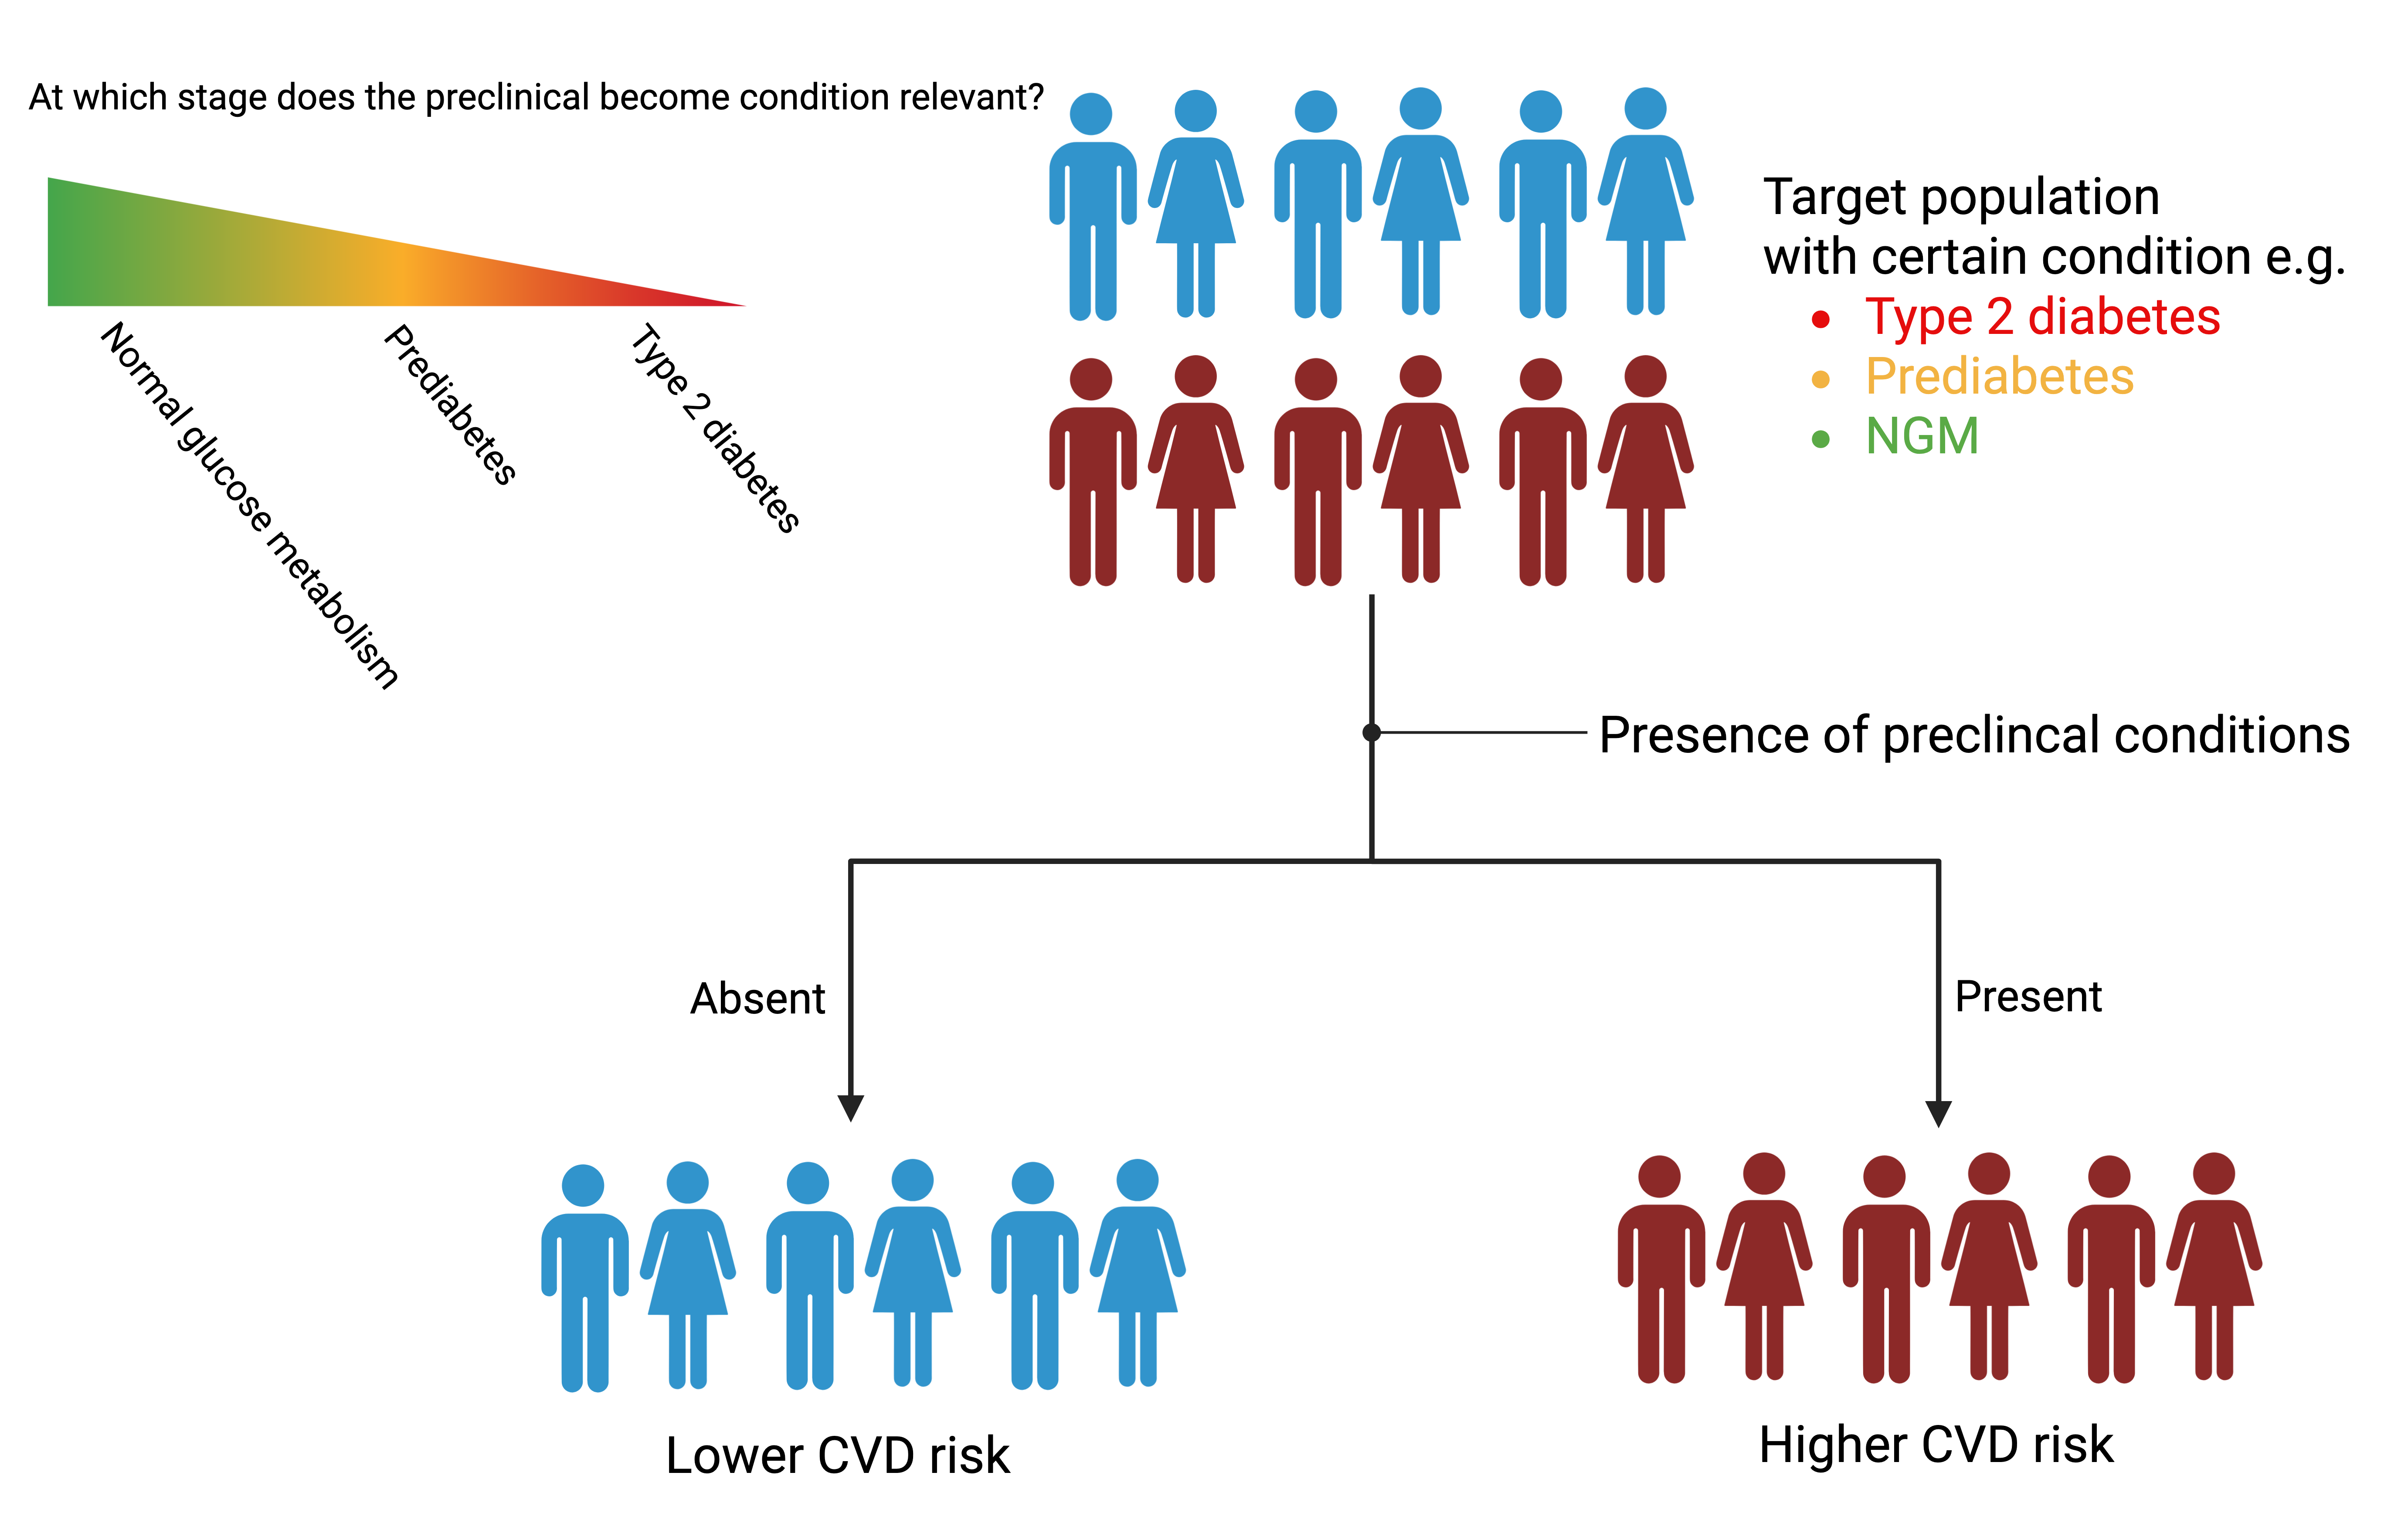
\includegraphics{images/risk_stratification.png}

}

\caption{Risk-stratification based on preclinical disease}

}

\end{minipage}%

\end{figure}

Cardiovascular autonomic dysfunction despite it's relationship with
cardiovascular complication has not been defined into clinical practice.
Larger epidemiological cohort studies encompassing various stages of
diabetes risk, from normal glucose metabolism to prediabetes, onset of
type 2 diabetes, and longer term progression of type 2 diabetes, serve
as valuable resources for identifying risk-stratification opportunities.
Epidemiological studies provide a broad representation of the target
population, allowing understand the relationship between cardiovascular
autonomic dysfunction and cardiovascular complications. They also have
potential to determine when, along the trajectory of diabetes
progression and duration, autonomic function are meaningful for
cardiovascular risk-stratification.

\hypertarget{aetiological-research}{%
\section{Aetiological research}\label{aetiological-research}}

Aetiology seeks to identify the causes and contributing factors of
disease, forming the foundation for understanding its development and
underlying mechanisms. Ideally, to determine causal effects, we would
compare outcomes in individuals who were exposed to a risk factor with
what would have happened if they had not been exposed. Since this
counterfactual scenario is impossible to observe directly, we rely on
study designs, such as randomized controlled trials when feasible, and
apply statistical methods to data from observational cohort studies to
approximate these comparisons. In cardiovascular disease,
socio-environmental influences and personal health behaviours play a
crucial role in overall health and are considered the outer contributing
layer to biological mechanism. The inner layer focuses on biological
causal processes, where the connection between these contributing
factors and individual predisposition to cardiovascular disease remains
a key question in understanding the underlying pathological mechanisms.

Cardiovascular autonomic dysfunction is linked to CVD and all-cause
mortality. However, many questions remain regarding the underlying
causal mechanisms. Furthermore, as dysglycemia is known to be a primary
driver of autonomic dysfunction\textsuperscript{19}, the questions is to
which extent it modulates the relationship between cardiovascular
autonomic dysfunction and CVD? This relationship remains unclear,
highlighting the need for a deeper understanding of this interplay in
target populations representing different stages of glucose metabolism.

\bookmarksetup{startatroot}

\hypertarget{aim-and-hypothesis}{%
\chapter{Aim and hypothesis}\label{aim-and-hypothesis}}

The overall aim of this PhD is to understand how cardiovascular
autonomic dysfunction/neuropathy (CAN) affects cardiovascular disease
risk (i.e.~heart failure, stroke, myocardial infarction) and specific
subclinical markers of CVD: carotid-femoral pulse wave velocity and
carotid artery distensibility in populations covering the whole glycemic
continuum, from healthy glucose metabolism to type 2 diabetes.

Study I: Quantify the cross-sectional association between 24-hour HRV
and subclinical markers of cardiovascular complications: carotid-femoral
pulse wave velocity and carotid artery distensibility, in a participants
with normoglycemia, prediabetes or type 2 diabetes.

Study II: Quantify the longitudinal association of week-long and hourly
HRV with incidence ischemic-CVD, heart failure, and all-cause mortality
in a population with high-risk of diabetes.

Study III: Quantify the cross-sectional association between CAN and
heart failure. Heart failure will be defined by clinical measures
i.e.~N-terminal-pro-BNP (Pro-BNP), WATCH-DM risk, and New York Heart
Association (NYHA) scores among individuals with type 2 diabetes.

The hypotheses of this dissertation are:

CAN and autonomic dysfunction is associated with CVD and acts as an
early risk factor for heart failure and other cardiovascular
complications, including stroke, and myocardial infarction in patients
with prediabetes and/or type 2 diabetes. In addition autonomic
dysfunction is associated with higher levels of carotid-femoral pulse
wave velocity and carotid artery distensibility.

\bookmarksetup{startatroot}

\hypertarget{materials-and-methods-needs-to-be-fine-tuned}{%
\chapter{Materials and methods {[}needs to be
fine-tuned{]}}\label{materials-and-methods-needs-to-be-fine-tuned}}

\hypertarget{overview-of-the-studies}{%
\section{Overview of the studies}\label{overview-of-the-studies}}

\begin{longtable}[]{@{}
  >{\raggedright\arraybackslash}p{(\columnwidth - 6\tabcolsep) * \real{0.0588}}
  >{\raggedright\arraybackslash}p{(\columnwidth - 6\tabcolsep) * \real{0.3095}}
  >{\raggedright\arraybackslash}p{(\columnwidth - 6\tabcolsep) * \real{0.3581}}
  >{\raggedright\arraybackslash}p{(\columnwidth - 6\tabcolsep) * \real{0.2685}}@{}}
\caption{Table 1: Overview of studies}\tabularnewline
\toprule\noalign{}
\begin{minipage}[b]{\linewidth}\raggedright
\end{minipage} & \begin{minipage}[b]{\linewidth}\raggedright
Study I
\end{minipage} & \begin{minipage}[b]{\linewidth}\raggedright
Study II
\end{minipage} & \begin{minipage}[b]{\linewidth}\raggedright
Study III
\end{minipage} \\
\midrule\noalign{}
\endfirsthead
\toprule\noalign{}
\begin{minipage}[b]{\linewidth}\raggedright
\end{minipage} & \begin{minipage}[b]{\linewidth}\raggedright
Study I
\end{minipage} & \begin{minipage}[b]{\linewidth}\raggedright
Study II
\end{minipage} & \begin{minipage}[b]{\linewidth}\raggedright
Study III
\end{minipage} \\
\midrule\noalign{}
\endhead
\bottomrule\noalign{}
\endlastfoot
Title & Cardiovascular autonomic dysfunction is linked with arterial
stiffness across glucose metabolism: The Maastricht Study &
Cardiovascular autonomic dysfunction precedes cardiovascular disease and
all-cause mortality: 11-year follow-up in the ADDITION-PRO study &
Cardiovascular autonomic neuropathy and subclinical heart failure in
type 2 diabetes: The CANCAN study \\
Design & Aetiological cross-sectional study & Aetiological prospective
cohort study & Descriptive cross-sectional study \\
Cohort & Maastricht study & ADDITION-PRO & CANCAN \\
Study population & 3673 people with normal glucose metabolism,
prediabetes, and type 2 diabetes & 2082 people with high risk of
diabetes & 173 patients with type 2 diabetes visiting outpatients
clinics \\
Data sources & Population-based cohort from The Maastricht Study in the
Netherlands & Cohort study of selected people based on having high risk
of diabetes & Clinical cohort study \\
Determinant & 24-hour HRV &
\multicolumn{2}{>{\raggedright\arraybackslash}p{(\columnwidth - 6\tabcolsep) * \real{0.6266} + 2\tabcolsep}@{}}{%
multiday and hourly HRV \textbar{} Cardiovascular autonomic reflex test
\textbar{}} \\
Primary outcome & Arterial stiffness & Major adverse cardiovascular
events, heart failure, and all-cause mortality & NT-proBNP \\
Statistical analysis & Linear regression & Poisson regression & Logistic
regression \\
Missing data & Complete case analysis & Multiple imputation of chained
equations for confounders & Complete case analysis and multiple
imputation of chained equations for CART and confounders \\
\end{longtable}

\hypertarget{study-population}{%
\subsection{Study population}\label{study-population}}

\begin{figure}

{\centering 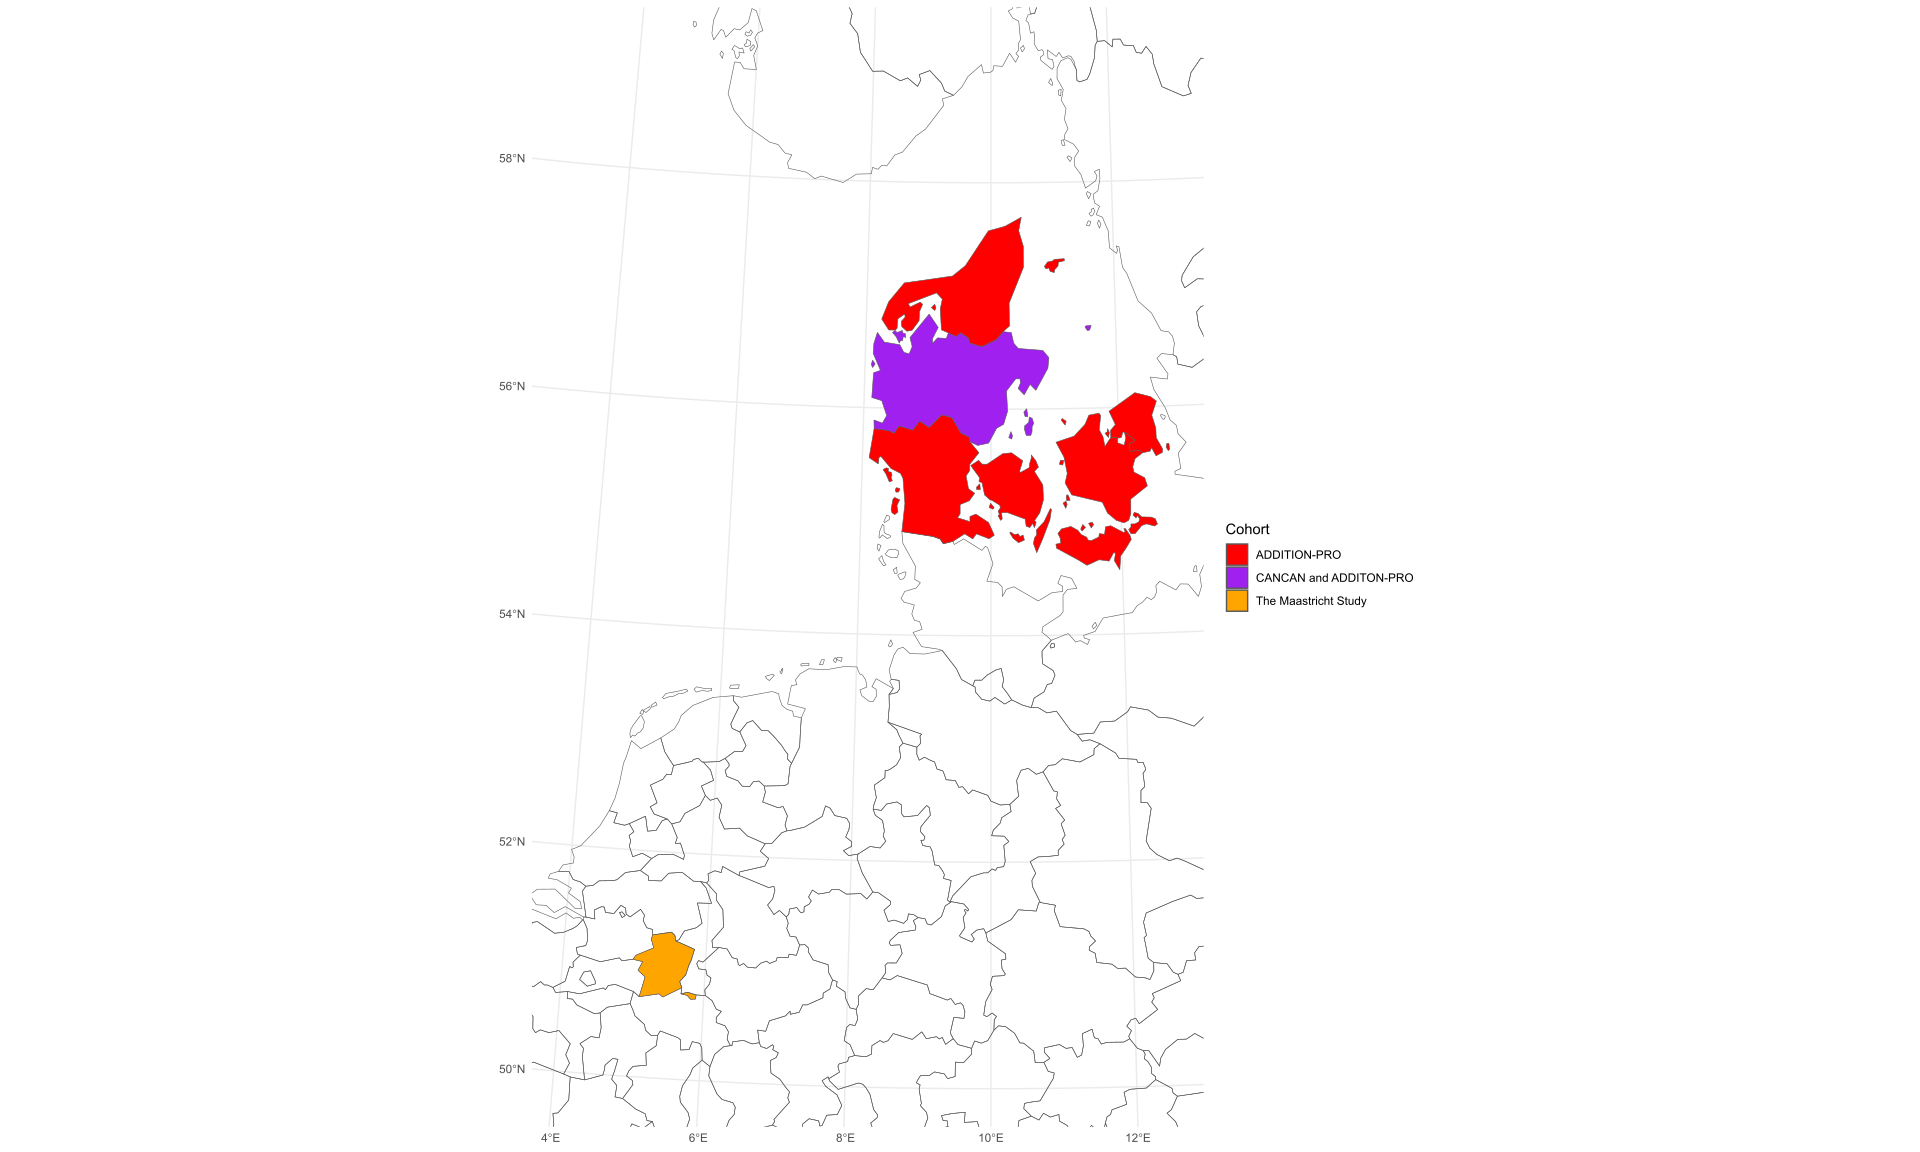
\includegraphics[width=8in,height=\textheight]{images/cohort_map.png}

}

\caption{Study populations}

\end{figure}

\hypertarget{study-i---the-maastricht-study}{%
\subsubsection{Study I - The Maastricht
Study}\label{study-i---the-maastricht-study}}

The Maastricht Study is a prospective observational population-based
study of the general population of the province of Limburg, in the
southern part of the Netherlands. The study emphasized the recruitment
of people with type 2 diabetes, through the regional Diabetes Patient
Registry, to extensively phenotype individuals with type 2 diabetes and
those in intermediate stages of the disease. The eligibility criteria
included an age range of 40--70 years. Participants were recruited
through mass media campaigns and mailings from municipal registries
(Gemeentelijke Basis Administratie; GBA). In the analysis of Study I,
the study among 7449 population included participants with measurements
of 24-hour HRV and at least one measure of arterial stiffness
(carotid-femoral pulse wave velocity or carotid artery distensibility),
both of which were completed within a three-month period between
November 2010 and December 2020. The study has been approved by the
institutional medical ethics committee (NL31329.068.10) and the Minister
of Health, Welfare and Sports of the Netherlands (Permit
131088-105234-PG). All participants gave written informed consent.

\hypertarget{study-ii---addition-pro}{%
\subsubsection{Study II - ADDITION-PRO}\label{study-ii---addition-pro}}

The ADDITION-PRO study is a prospective population-based cohort nested
within the Danish arm of the ADDITION-Europe study, originally designed
as a stepwise screening program for type 2 diabetes in general practice.
ADDITION-PRO aims to investigate early markers of cardiovascular disease
(CVD) and metabolic dysfunction in individuals in different tiers of
diabetes risk.

The ADDITION-Europe screening program identified a large number of
individuals with impaired fasting glucose (IFG), impaired glucose
tolerance (IGT), and normoglycemia despite having risk factors for
diabetes and CVD. Participants for ADDITION-PRO were recruited from the
original ADDITION-DK screening cohort, which included individuals from
190 general practices across Denmark. The recruitment strategy focused
on individuals at high risk of diabetes without type 2 diabetes,
identified through a stepwise screening program that incorporated the
Danish diabetes risk score from the Inter99. This assessment, conducted
between 2001 and 2006, considered factors such as age, sex, history of
gestational diabetes, family history of diabetes, known hypertension,
BMI, and physical activity. High risk individuals were further screened
for type 2 diabetes by blood measurements including HbA1c, random blood
glucose, FPG, and OGTT, were identified patients were invited to the
ADDITION-trial. High risk individuals without type 2 diabetes were
further considered in as the sampling frame for ADDITION-PRO.

Between 2009 and 2011, a follow-up health examination was conducted at
four ADDITION-DK study centers to establish a longitudinal cohort.
Eligible participants were those still alive, residing near the research
centers (Steno Diabetes Center Copenhagen, Aarhus University Hospital,
Holstebro Hospital, and the Hospital of South West Jutland, Esbjerg),
and who had not withdrawn consent. Eligibility criteria included
individuals aged 40--70 years who had previously undergone diabetes
screening in ADDITION-DK. Exclusion criteria included pregnancy,
psychological or psychiatric disorder preventing informed consent, and
life-limiting conditions. One key feature of the data collection was the
precise measurement of physical activity and energy expenditure using
ActiHeart, which recorded acceleration and heart rate over a week. In
study II, we included participants with a least 48-hour recording for
our first analysis, and then include those participants with hourly
measures of physical acceleration during the hourly HRV recording for th
second analysis. We also excluded participant with prior CVD ten years
before inclusion.

The population were disease history and follow-up in the unique register
system of Denmark, which allows linkage of health records using the
personal Civil Registration Number assigned to all citizens. The
following national registries were accessed to collect information on
incident CVD and mortality, medication use, and healthcare utilization:
the National Patient Registry (hospital admissions and outpatient
contacts), the National Health Service Registry (general practice
visits), the Medical Prescription Registry, the Diabetes Registry, and
the Cause of Death Registry.

\hypertarget{study-iii---cancan}{%
\subsubsection{Study III - CANCAN}\label{study-iii---cancan}}

The CANCAN Study is an observational pilot study conducted at two
hospital outpatient clinics in Viborg Regional Hospital and Regional
Hospital Gødstrup. It aims to implement a screening protocol for
identifying high-risk individuals using CAN assessments, continuous
glucose monitoring, and heart failure indicators. All measures were part
of routine clinical care for type 2 diabetes in Central Denmark. We
included 200 adults (\textgreater18 years) with type 2 diabetes with
duration of over one year. Exclusion criteria were recent laser-treated
eye disease (≤3 months), pregnancy, lactation, life-threatening illness,
or cognitive impairment preventing consent. Participants were identified
via electronic records and informed about the study by their doctor
during a telephone call. Those interested attended a dedicated meeting
before their annual diabetes exam, where study details were discussed.
Recruitment took place from 2021 to 2024. In study III, participants
without a valid NT-proBNP measurement were excluded.

\hypertarget{study-variables}{%
\section{Study variables}\label{study-variables}}

\hypertarget{measures-for-cardiovascular-autonomic-dysfunction-neuropathy}{%
\subsection{Measures for cardiovascular autonomic dysfunction/
neuropathy}\label{measures-for-cardiovascular-autonomic-dysfunction-neuropathy}}

\textbf{Heart rate variability}

\begin{figure}

\begin{minipage}[t]{\linewidth}

{\centering 

\raisebox{-\height}{

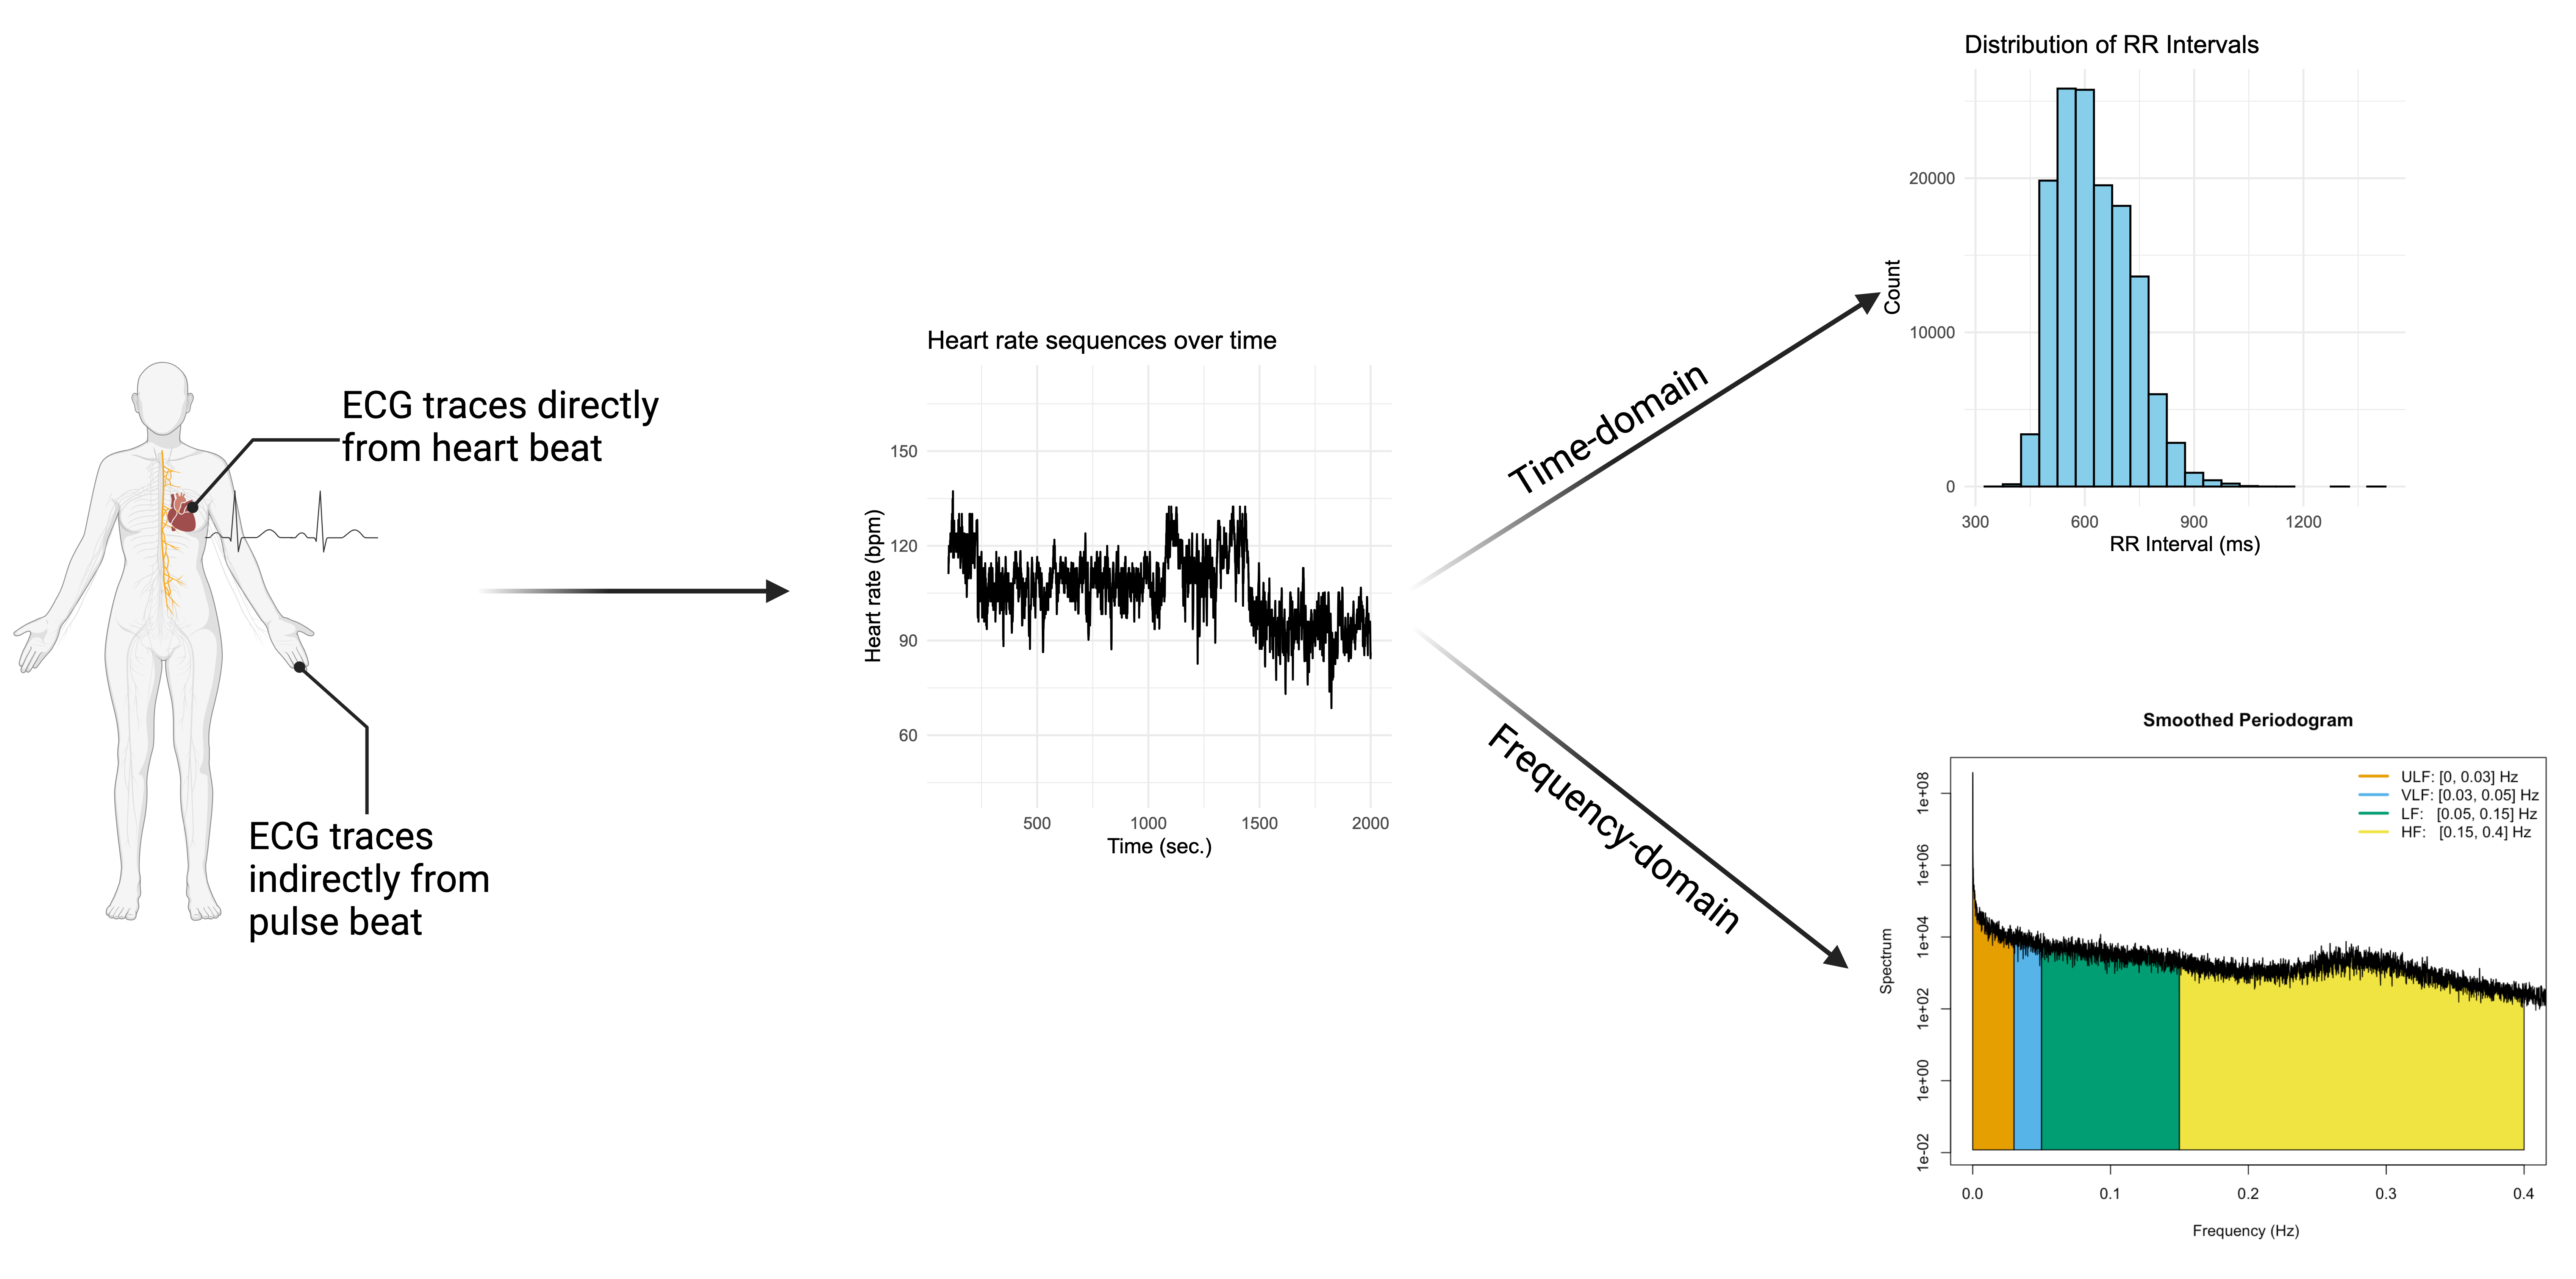
\includegraphics[width=8in,height=\textheight]{images/measurements_hrv.png}

}

\caption{Heart rate variability}

}

\end{minipage}%

\end{figure}

In study I-III a device was used to capture the distance between each
heartbeat defined as RR intervals from electrocardiogram traces either
directly from heart-beat traces or indirectly from pulse traces. From
this a sequence of successive heart beat intervals is extracted to
calculate HRV. The pool of hearbeat data, we extrapolated time-domain
and frequency-domain HRV indices. In study III, we used the ratio in
pulse rate in test under different conditions lying-to-stading, in-
expiration, and valsalva maneuvre.

\emph{Time-domain indices}

Time-domain measures of HRV are based on the statistical distribution of
normal-to-normal (NN) heartbeat intervals. Description of time-domain
indices are summarized in box 1.

\begin{longtable}[]{@{}
  >{\raggedright\arraybackslash}p{(\columnwidth - 2\tabcolsep) * \real{0.5000}}
  >{\raggedright\arraybackslash}p{(\columnwidth - 2\tabcolsep) * \real{0.5000}}@{}}
\caption{Box 1: Time-domain HRV indices}\tabularnewline
\toprule\noalign{}
\begin{minipage}[b]{\linewidth}\raggedright
Time-domain HRV
\end{minipage} & \begin{minipage}[b]{\linewidth}\raggedright
Description
\end{minipage} \\
\midrule\noalign{}
\endfirsthead
\toprule\noalign{}
\begin{minipage}[b]{\linewidth}\raggedright
Time-domain HRV
\end{minipage} & \begin{minipage}[b]{\linewidth}\raggedright
Description
\end{minipage} \\
\midrule\noalign{}
\endhead
\bottomrule\noalign{}
\endlastfoot
\textbf{Standard deviation of NN heart beat intervals (SDNN, in ms)} &
Reflects overall HRV and total autonomic nervous system activity over
the recording period. \\
\textbf{SD of the averages of NN intervals in 5-minute segments
throughout the recording (SDANN, in ms)} & Measures long-term HRV
variations, primarily reflecting circadian and autonomic
fluctuations. \\
\textbf{Mean of the SDs of all NN intervals for all 5-minute segments
(SDNN index, in ms)} & Estimates short-term HRV fluctuations and vagal
tone by averaging segmental variations. \\
\textbf{NN50 count divided by the total number of all NN intervals
(pNN50, percentage)} & Represents the proportion of successive NN
intervals differing by more than 50 ms, indicating vagal activity. \\
\textbf{Square root of the mean of the sum of squares of differences
between adjacent NN intervals (RMSSD, in ms)} & Reflects short-term HRV,
mainly parasympathetic (vagal) activity. \\
\end{longtable}

\emph{Frequency-domain indices}

Frequency-domain HRV indices are derived from sequences of NN intervals
transformed into the spectral domain using Fourier transformation. These
indices quantify heart rate oscillations over different timescales.
Short-term variations, such as respiratory sinus arrhythmia, reflect
rapid autonomic changes, while longer oscillations capture autonomic
responses to posture changes, circadian rhythms, or other physiological
processes. Description of frequency-domain indices are summarized in box
2.

\begin{longtable}[]{@{}
  >{\raggedright\arraybackslash}p{(\columnwidth - 2\tabcolsep) * \real{0.3465}}
  >{\raggedright\arraybackslash}p{(\columnwidth - 2\tabcolsep) * \real{0.6535}}@{}}
\caption{Box 2: Frequency-domain HRV indices}\tabularnewline
\toprule\noalign{}
\begin{minipage}[b]{\linewidth}\raggedright
Frequency domain HRV
\end{minipage} & \begin{minipage}[b]{\linewidth}\raggedright
Description
\end{minipage} \\
\midrule\noalign{}
\endfirsthead
\toprule\noalign{}
\begin{minipage}[b]{\linewidth}\raggedright
Frequency domain HRV
\end{minipage} & \begin{minipage}[b]{\linewidth}\raggedright
Description
\end{minipage} \\
\midrule\noalign{}
\endhead
\bottomrule\noalign{}
\endlastfoot
\textbf{Variance of all NN intervals ≤ 0.4 Hz, total power (TP, in ms²)}
& Represents overall HRV, reflecting both short- and long-term autonomic
regulation. \\
\textbf{Ultralow-frequency range (ULF, in ms² ≤ 0.003 Hz)} & Captures
very long-term oscillations, influenced by circadian rhythms,
metabolism, and thermoregulation. \\
\textbf{Very-low-frequency range (VLF, in ms²; 0.003--0.04 Hz)} &
Associated with sympathetic activity, inflammation, and hormonal
regulation. \\
\textbf{Low-frequency range (LF, in ms²; 0.04--0.15 Hz)} & Reflects a
mix of sympathetic and parasympathetic activity, often linked to blood
pressure regulation and baroreflex sensitivity. \\
\textbf{High-frequency range (HF, in ms²; 0.15--0.4 Hz)} & Represents
parasympathetic (vagal) modulation of heart rate, closely related to
respiratory sinus arrhythmia. \\
\end{longtable}

\textbf{Holter recordings in study I}

All ECG recordings were obtained using a 12-lead Holter system
(Fysiologic ECG Services, Amsterdam, the Netherlands) over 24 hours, as
previously described. Participants were instructed to follow their
regular daily activities but avoid showering during the recording. The
ECG data were processed using proprietary Holter Analysis Software
(Fysiologic ECG Services), where artefacts and ectopic beats were
excluded through automated processing and manual validation. A minimum
recording duration of 18 hours was required for further analysis.
Inter-beat intervals between consecutive sinus beats were provided in
milliseconds (ms). Time-domain HRV indices were calculated, including
SDNN, SDANN, RMSSD, SDNN index, and pNN50. Frequency-domain measures
were derived using Fast Fourier Transform, including TP, ULF, VLF, LF,
and HF. Outliers were removed. HRV indices were standardised by their
mean and SD, and composite Z-scores were computed for time and
frequency-domain measures, respectively. This selection of indices
covers the main sources of HRV variance.

\textbf{ActiHeart heart rate and physical activity in study II}

Heart rate was measured using a combined accelerometer and heart rate
monitor (ActiHeart, CamNTech, Cambridge, UK), recording uniaxial
acceleration and heart rate. The data collection and processing methods
have been described previously. Mean heart rates were recorded in
30-second epochs, and HRV was derived as the variation between
consecutive normal heartbeats on the ECG. HRV calculations were
performed using the RHRV package (version 4.2.7) in R, including SDNN,
SDANN, SDNN index, TINN, and mean HR (mHR). We tested our approach on a
dataset with full access to all interbeat intervals to validate our
algorithm\textsuperscript{20}. These indices have shown high validity
for HRV indices based on global distribution (e.g.~SDNN, SDANN, SDNNi)
in 24-hour recordings. HRV indices were calculated by week, 24-hour
cycle, and hour of the day, with hourly values averaged across recording
days.

\textbf{Vagus device for cardiovascular autonomic reflex test in study
III}

CAN was diagnosed using cardiovascular autonomic reflex tests (CARTs),
the gold standard for CAN assessment. R-R intervals were derived from an
ECG signal using the Vagus™ device (Medicus Engineering, Aarhus,
Denmark). Three standardized CARTs were performed: lying-to-standing,
deep breathing, and the Valsalva manoeuvre, following a standardized
protocol between 8:00 a.m. and 2:00 p.m. after 10 minutes of supine
rest. Smoking and caffeine intake were prohibited two hours before
testing. Each test was conducted once by trained examiners.

\begin{figure}

{\centering 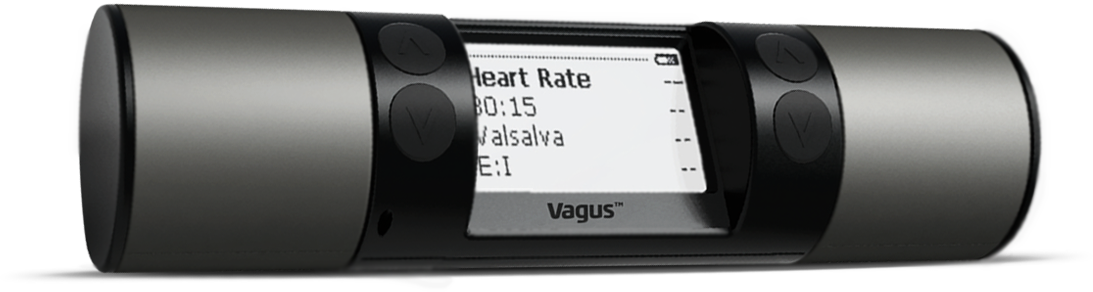
\includegraphics[width=2in,height=\textheight]{images/vagus_device.png}

}

\caption{Handheld Vagus™ device}

\end{figure}

Manifest CAN was defined as two or more abnormal CARTs using
age-specific cut-off values (ref.). The Vagus™ device's accuracy has
been validated against FDA standards and stationary devices, showing
moderate to high reproducibility (ref.).

\begin{figure}

\begin{minipage}[t]{\linewidth}

{\centering 

\raisebox{-\height}{

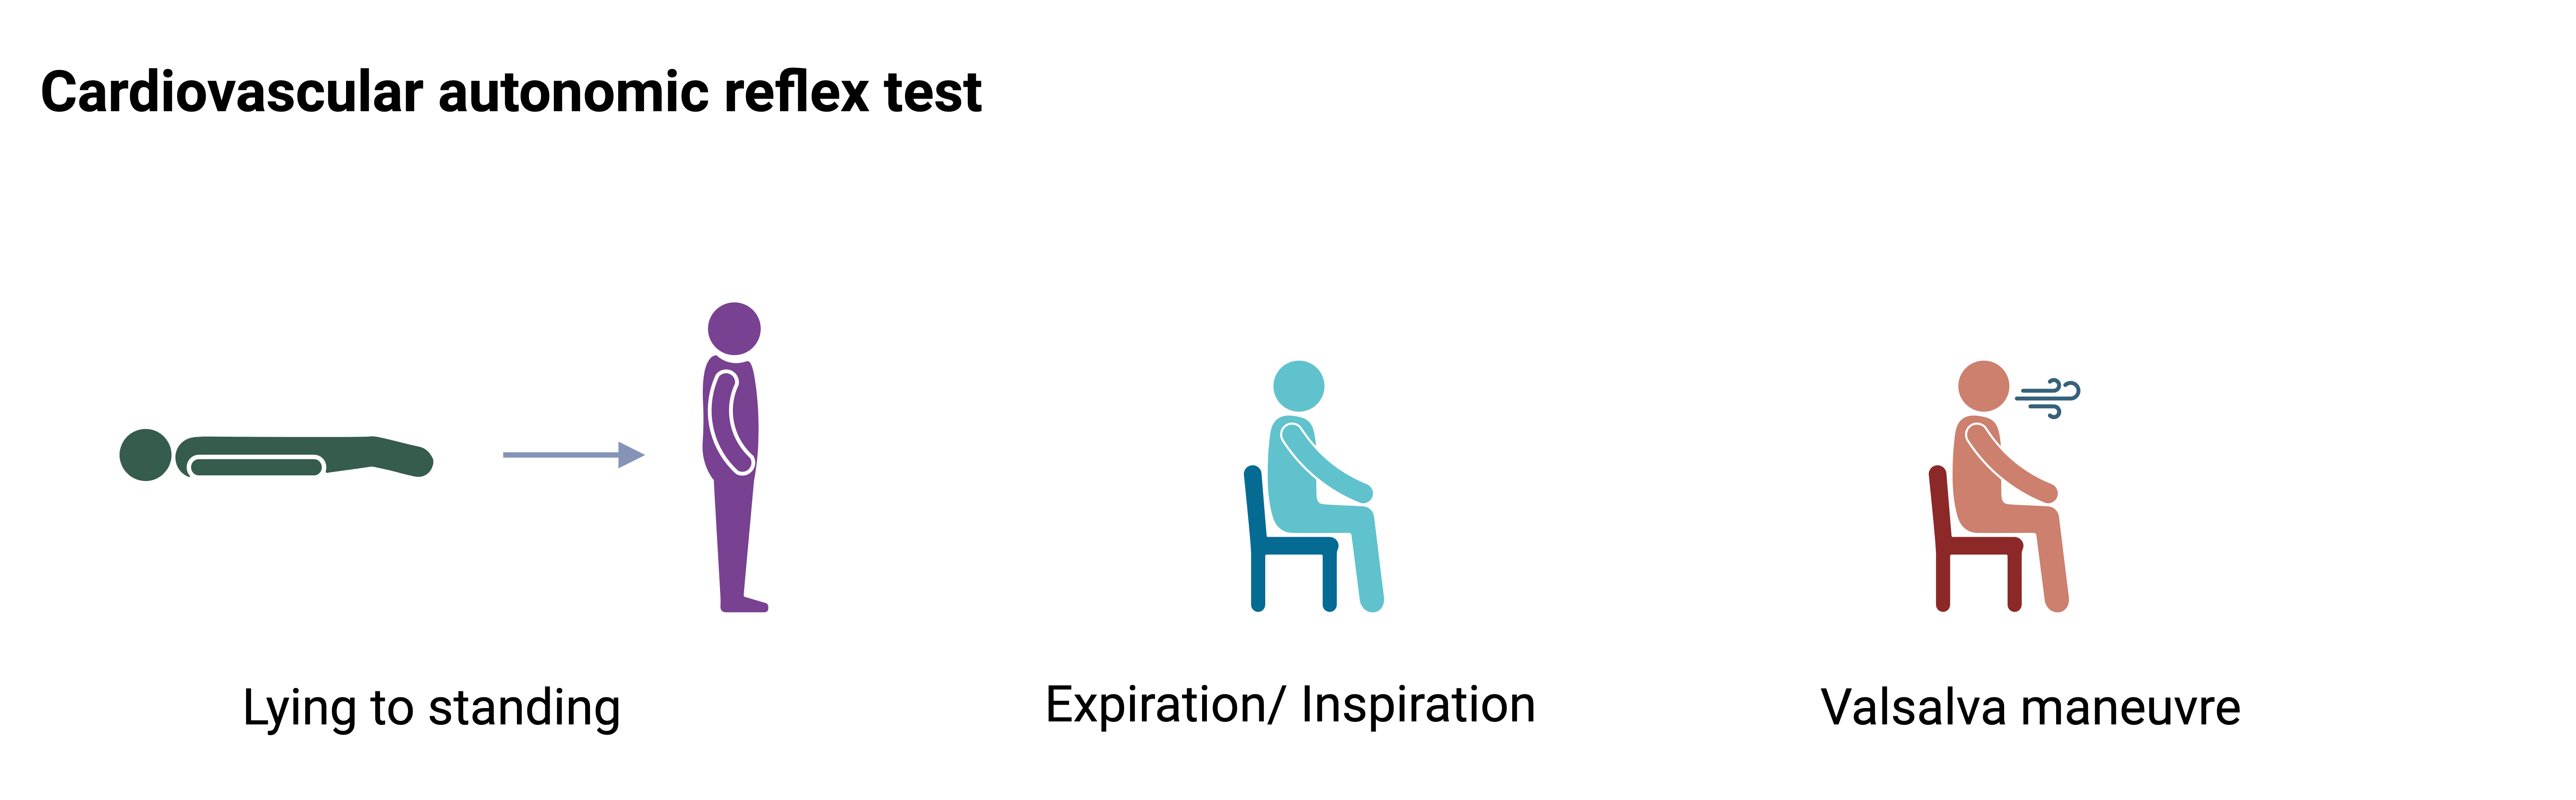
\includegraphics{images/cart.png}

}

\caption{CART}

}

\end{minipage}%

\end{figure}

HRV was derived from all CARTs using autoregressive spectral analysis.
Time domain measures included SDNN and RMSSD, while frequency domain
measures included LF, HF, and total power. Orthostatic hypertension was
defined as a sustained drop in systolic blood pressure of ≥20 mmHg or
diastolic blood pressure of ≥10 mmHg within three minutes of standing
(ref.).

\hypertarget{confounders-and-variables-for-instrumental-bias}{%
\subsection{Confounders and variables for instrumental
bias}\label{confounders-and-variables-for-instrumental-bias}}

Across Studies I, II, and III, a comprehensive set of covariates and
potential confounders were assessed, including lifestyle factors,
clinical measurements, biochemical markers, and socioeconomic
indicators.

Smoking status was self-reported in all studies, categorized as never,
former, or current (Study I), current/ex/never (Study II), and
smoker/non-smoker (Study III). Alcohol consumption was recorded as
average weekly units in all three studies. Physical activity was
assessed via self-report in Studies I, II, III, with Study I capturing
total and moderate-to-vigorous activity (hours/week), Study II used the
Recent Physical Activity Questionnaire (RPAQ) to calculate physical
activity energy expenditure (PAEE), and Study III classifying activity
as sedentary or non-sedentary. In Study II also used combined
accelerometry and heart rate monitoring (ActiHeart) to estimate PAEE.
Study II included register-based data on socioeconomic status at
baseline, including education length, income, and employment status. All
studies included measurements of body mass index (BMI), waist
circumference, and systolic and diastolic blood pressure, obtained
during clinical examinations.

Blood samples were analyzed in all studies for HbA1c, fasting plasma
glucose (FPG), triglycerides, total cholesterol, high-density
lipoprotein (HDL), and low-density lipoprotein (LDL) cholesterol. Study
I also included a 2-hour oral glucose tolerance test (OGTT) to classify
glucose metabolism status based on FPG and OGTT (normal, prediabetes,
type 2 diabetes) using WHO 2006 criteria, excluding HbA1c as a
diagnostic criterion. Study III additionally measured creatinine,
estimated glomerular filtration rate (eGFR), and urine
albumin-to-creatinine ratio.

Self-reported history of cardiovascular disease (CVD) and use of
anti-hypertensive, glucose-lowering, and lipid-lowering medications were
collected in all studies. In study II, history of CVD events in the 10
years prior to baseline were retrieved from national registers. In study
III, history of CVD was collected electronic patient records.

\hypertarget{outcomes}{%
\section{Outcomes}\label{outcomes}}

\hypertarget{arterial-stiffness}{%
\subsection{Arterial stiffness}\label{arterial-stiffness}}

\textbf{Pulse wave velocity}

Arterial stiffness can be characterized by measuring arteriosclerosis
and atherosclerosis properties of the arteries. The stiffness of
different trees of the vascular musculature can assessed both locally
and dynamically. Aortic and carotid stiffness were assessed as markers
of arterial stiffness, following previously described procedures. Aortic
stiffness was measured by carotid-femoral pulse wave velocity (PWV)
using applanation tonometry (SphygmoCor, Atcor Medical, Sydney,
Australia), with the median of at least three consecutive recordings
included in the analysis.

\textbf{Carotid artery distensibility}

Carotid stiffness was assessed by the carotid artery distensibility
coefficient (CD), based on ultrasound imaging of the left common carotid
artery using a 7.5 MHz linear probe (MyLab 70, Esaote Europe,
Maastricht, the Netherlands). CD was calculated as ΔD/braPP, where ΔD
represents carotid distension and braPP is brachial pulse pressure. Mean
heart rate and mean arterial pressure (MAP) were recorded every five
minutes using an oscillometer device (Accutorr Plus, Datascope,
Montvale, NJ, USA).

\begin{figure}

\begin{minipage}[t]{\linewidth}

{\centering 

\raisebox{-\height}{

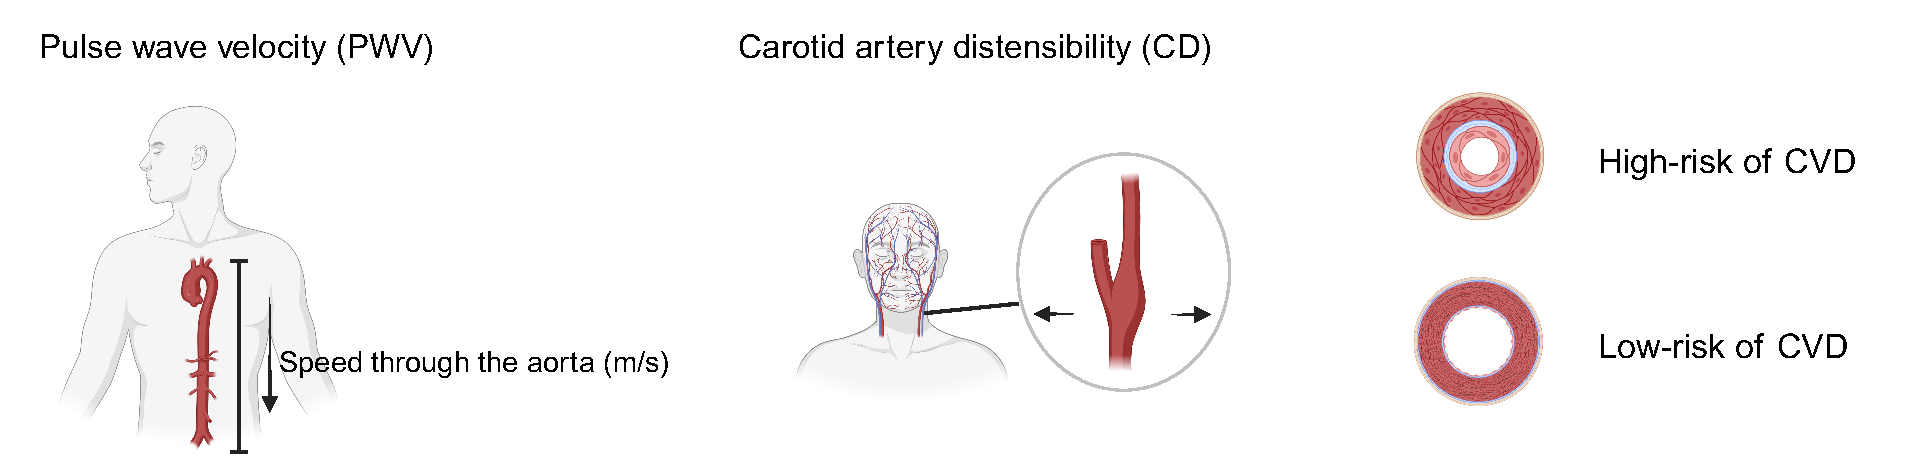
\includegraphics{images/Methods_arterial_stiffness.pdf}

}

\caption{description missing}

}

\end{minipage}%

\end{figure}

\hypertarget{biomarker-of-heart-failure}{%
\subsection{Biomarker of heart
failure}\label{biomarker-of-heart-failure}}

N-terminal prohormone of brain natriuretic peptide (NT-proBNP) is a
neuretic peptide that can be used to detect patients with heart failure
and the progression. It derives from B-type natriuretic peptid (BNP)
which is a cardial neurohormon, that is syntezied and secreted as
response to streched cariomycytes and cardiac volume overload. After
secretion, proBNP is cleaved, releasing the active hormone BNP along
with the remaining N-terminal fragment, known as NT-proBNP. In study
III, blood sample were taken at study cite. Description of the NT-proBNP
analysis of plasma samples is described in supplementary material
{[}ref.{]}.

\hypertarget{cardiovascular-events}{%
\subsection{Cardiovascular events}\label{cardiovascular-events}}

Information on CVD events and mortality was obtained from the Danish
National Patient Registers until 2021. ICD-10 codes for stroke,
myocardial infarction, cardiovascular death, cardiovascular
revascularization, and heart failure. We defined three-point major
adverse cardiovascular events (MACE) as myocardial infarction, stroke,
cardiovascular revascularization, and cardiovascular death.

\begin{longtable}[]{@{}
  >{\raggedright\arraybackslash}p{(\columnwidth - 2\tabcolsep) * \real{0.2267}}
  >{\raggedright\arraybackslash}p{(\columnwidth - 2\tabcolsep) * \real{0.7733}}@{}}
\toprule\noalign{}
\endhead
\bottomrule\noalign{}
\endlastfoot
\textbf{Outcome} & \textbf{Diagnosis codes} \\
\emph{Heart failure} & ICD: I50 \textbar{} \\
\emph{Three-point MACE} & \\
\begin{minipage}[t]{\linewidth}\raggedright
\begin{itemize}
\tightlist
\item
  Stroke
\end{itemize}
\end{minipage} & ICD: I61 - I64 \textbar{} \\
\begin{minipage}[t]{\linewidth}\raggedright
\begin{itemize}
\tightlist
\item
  Myocardial infarction
\end{itemize}
\end{minipage} & ICD: I21-I24 \textbar{} \\
\begin{minipage}[t]{\linewidth}\raggedright
\begin{itemize}
\tightlist
\item
  Cardiovascular death
\end{itemize}
\end{minipage} & ICD: I20-I28, I42, I46 \\
\begin{minipage}[t]{\linewidth}\raggedright
\begin{itemize}
\tightlist
\item
  Cardiovascular revascularization
\end{itemize}
\end{minipage} & SKA: KPAE10, KPAE25, KPAF10, KPAF20, KPAF21, KPAF22,
KPAH10, KPAH20, KPAH21, KPEE, KPEF, KPEH, KPEP, KPEQ, KPFE,, KPFH, KPFP,
KPFQ \\
\end{longtable}

\hypertarget{statistical-methods}{%
\section{Statistical Methods}\label{statistical-methods}}

\hypertarget{cross-sectional-analysis}{%
\subsection{Cross-sectional analysis}\label{cross-sectional-analysis}}

In study I, we used multiple linear regression to investigate
associations between multiday HRV and arterial stiffness. Model 1
adjusted for age, sex, education, glucose metabolism status, and mean
arterial pressure (MAP) to account for the oversampling of individuals
with type 2 diabetes and potential instrumental bias of arterial
pressure flow. Model 2 included additional adjustments for smoking
behavior, alcohol consumption, physical activity, body mass index,
HbA1c, triglycerides, total-to-HDL cholesterol ratio, and medication
use. Arterial stiffness measures were log-transformed to ensure normally
distributed residuals and back-transformed into percentage change
estimates. We add interaction sex to oberve if the association differed
between sex. We performed sensitivity analyses excluding individuals on
antihypertensive treatment or glucose-lowering medication. In study III,
we applied logistic regression models to investigate the association
between CAN and heart failure, using NT-proBNP as the primary outcome.
We adjusted for age, sex, and diabetes duration, smoking behavior,
alcohol consumption, body mass index, HbA1c, triglycerides, total
cholesterol, and antihypertensive medication, eGFR and prior CVD. We
performed sensitivity analyses excluded participants with beta-blocker
treatment or prior CVD.

\hypertarget{time-to-event-analysis}{%
\subsection{Time-to-event analysis}\label{time-to-event-analysis}}

In study II, we used Poisson regression models to quantify the
associations between HRV and cardiovascular events, as follow-up data
were undisturbed over time and to avoid assumptions of proportional
hazards\textsuperscript{21}. Multiday HRV was modelled using splines
with knots at predefined percentiles to assess non-linear associations.
Hourly HRV was analysed separately for each hour to observe if the
association of HRV had diurnal variation. Both HRV and mHR were
standardized by their mean and standard deviation to ensure
comparability. Based on assumptions about potential confounding pathways
summarized in directed acyclic graphs (DAG), we fitted two models: Model
1 adjusted for age and sex, while Model 2 further adjusted for
education, smoking, alcohol consumption, physical activity (physical
activity energy expenditure (PAEE) calculated from Recent Physical
Activity Questionnaire RPAQ), body mass index, total cholesterol, and
HbA1c. Additional analyses were performed with HRV pre-adjusted for
concurrent heart rate and physical acceleration to account the influence
of these factors. Missing covariates were handled using multiple
imputation. {[}Add age specific incidence rates{]}

\hypertarget{effect-modification}{%
\subsection{Effect modification}\label{effect-modification}}

Effect modification is used to assess whether the association between an
exposure and an outcome varies depending on the level of a third
variable, known as the effect modifier. This means that the observed
relationship between the exposure and the outcome is not uniform across
all subgroups. Instead, it differs across strata defined by the effect
modifier\textsuperscript{22}.

In study I, we hypothesize that the association between 24-hour and
arterial stiffness was stronger in strata of progression of diabetes
(normal glucose metabolism, prediabetes, type 2 diabetes). We therefore
first stratified by diabetes status to observe the size of the
association across strata. We then combine all groups and include an
interaction term between HRV and diabetes status. We did subsidiary
analysis to check if the effect was modified by dysglycemia by
stratifying HbA1c and fasting plasma glucose into deciles. In Study II,
we quatified whether the association between multiday HRV and CVD
endpoints varied by sex to explore potential biological dimorphism.

In Study III, we aimed to determine whether the association between CAN
and elevated NT-proBNP is present in the subgroup without symptoms,
defined as NYHA class \textless{} II. Hence, we hypothesized no
significant effect modification between groups with and without
symptoms. Similarly, we explored whether the association remains present
in the group classified as low to moderate risk of heart failure, based
on the WATCH-DM risk score.

A significant effect modification between the exposure and the effect
modifier in all analyses was defined as an interaction term with a
p-value \textless{} 0.05.

\hypertarget{multiple-imputed-by-chained-equations}{%
\subsection{Multiple imputed by chained
equations}\label{multiple-imputed-by-chained-equations}}

Multiple Imputation by Chained Equations (MICE) is a method for handling
missing data in datasets. This procedure imputes missing values through
an iterative series of predictive models, generating plausible estimates
while preserving the relationships within the data. To avoid one
imputation for missing value could give the value the same confidence as
the a non-missing value, we followed Rubins Rule. Rubin's rules in MICE
combine results from multiple imputed datasets by pooling estimates of
interest (e.g., means or regression coefficients) using their within-
and between-imputation variances. Thus, we ensure valid statistical
inferences by accounting for the uncertainty introduced by missing data.

In study II, we imputed confounders to include as many participants and
avoid excluding population with our without cardiovascular or mortality
events. We imputed dataset 10 times. In study III, we imputed missing
CART, as a proportion of participants had non-valid test due to
insufficient air in the valsalva manuevre, unstable heart beats or data
error. These variables was used as auxiliary variables in imputation to
reduce bias\textsuperscript{23}. All available variables of biochemical
measures, diagnosis, medication and cause of non-valid CART was used to
impute each missing CART using predictive mean matching.

\hypertarget{instrumental-bias}{%
\subsection{Instrumental bias}\label{instrumental-bias}}

In study I-III we are investigating the body properties by dynamic
measures and biomarkers to quantify autonomic function, arterial
stiffness, and cardiac function. Other conditions may affect the
properties we are attempting to measure, and thus are causing
instrumental bias.

\emph{Vascular Stiffness}

In Study I, we used measurements of arterial stiffness using cf-PWV and
carotid distensibilty. Both measures are influenced by arterial pressure
at the time of examination. Arterial pressure affects the propagation of
the pressure wave through the aorta (cf-PWV) and the expansion and
contraction of the carotid artery (carotid distensibilty.) {[}ref.{]}.
To account for this, we adjusted for mean arterial pressure in our
models.

\emph{Cardiovascular autonomic function}

In Study II, we assessed cardiovascular autonomic function using
multiday HRV recordings and hourly HRV measurements. Studies have
highlighted that HRV is dependent on heart rate, and low HRV may simply
reflect a higher resting heart rate (rHR). To adjust for this without
overcorrecting for a collinear variable, we pre-adjusted HRV by
regressing rHR on HRV, extracting the residuals, and using these as the
pre-adjusted determinant. For hourly HRV, variability in heart rate may
be influenced by changes in physical activity, creating a risk that HRV
serves as a proxy for movement rather than autonomic function. To
address this, we applied a similar pre-adjustment approach by regressing
concurrent heart rate and physical acceleration to account for physical
activity.

\emph{Biomarker of Heart Failure}

In Study III, kidney function and overweight are know to influence
NT-proBNP levels independently of heart failure. We adjusted the model
to account for the blurred effect of eGFR on NT-proBNP levels in the
analysis.

\bookmarksetup{startatroot}

\hypertarget{results-needs-to-be-fine-tuned}{%
\chapter{Results {[}needs to be
fine-tuned{]}}\label{results-needs-to-be-fine-tuned}}

In this section, I will summarize study population characteristics and
findings from analysis.

\hypertarget{study-i-1}{%
\section{Study I}\label{study-i-1}}

\hypertarget{descriptive}{%
\subsection{Descriptive}\label{descriptive}}

In The Maastricht Study, {[}10,000 participated by Date{]}, of those
1316 reported prior CVD. Participants who had valid 24-hour HRV measured
was 4379 and of those 3673 had a valid measurement of either CD or PWV.
Study population included 3673 participants. Further characteristic are
described in the study I manuscript {[}Table 1{]} {[}refeernce to study
I{]}.

\begin{table}
\centering
\resizebox{\linewidth}{!}{
\begin{tabular}{l|l|l|l}
\hline
**Characteristic** & **Normal glucose metabolism**  
N = 2,389 & **Prediabetes**  
N = 538 & **Type 2 Diabetes**  
N = 746\\
\hline
Sex &  &  & \\
\hline
Men & 1,028 (43\%) & 280 (52\%) & 481 (64\%)\\
\hline
Women & 1,361 (57\%) & 258 (48\%) & 265 (36\%)\\
\hline
Age (years) & 58 (51, 64) & 62 (57, 68) & 63 (57, 68)\\
\hline
Total physical activity (hours/week) & 13 (9, 19) & 13 (9, 19) & 12 (7, 17)\\
\hline
Moderate to vigorous physical activity (hours/week) & 5.3 (3.0, 8.3) & 4.5 (2.3, 7.5) & 3.8 (1.5, 6.8)\\
\hline
BMI (kg/m²) & 25.0 (22.9, 27.4) & 27.2 (24.9, 30.1) & 28.8 (26.0, 31.7)\\
\hline
Waist (cm) & 89 (81, 97) & 98 (90, 105) & 103 (96, 112)\\
\hline
HbA1c (\%) & 5.35 (5.17, 5.63) & 5.63 (5.35, 5.90) & 6.54 (6.08, 7.09)\\
\hline
Fasting plasma glucose (mmol/L) & 5.10 (4.80, 5.40) & 5.90 (5.40, 6.30) & 7.40 (6.60, 8.50)\\
\hline
LDL (mmol/L) & 3.20 (2.70, 3.90) & 3.30 (2.60, 4.00) & 2.40 (1.80, 3.10)\\
\hline
HDL (mmol/L) & 1.60 (1.30, 2.00) & 1.40 (1.20, 1.80) & 1.30 (1.00, 1.50)\\
\hline
Total cholesterol (mmol/L) & 5.50 (4.80, 6.20) & 5.50 (4.80, 6.30) & 4.50 (3.90, 5.20)\\
\hline
Triglycerides (mmol/L) & 1.05 (0.80, 1.45) & 1.39 (1.03, 1.90) & 1.51 (1.08, 2.14)\\
\hline
Duration of type-2 diabetes (only for diagnosed participants) & NA (NA, NA) & NA (NA, NA) & 3 (0, 9)\\
\hline
Mean IBI (ms) & 838 (775, 907) & 815 (760, 897) & 806 (744, 889)\\
\hline
SDNN (ms) & 138 (117, 164) & 127 (106, 152) & 116 (96, 139)\\
\hline
RMSSD (ms) & 26 (21, 34) & 24 (19, 33) & 22 (17, 31)\\
\hline
SDANN (ms) & 125 (103, 149) & 113 (92, 139) & 103 (84, 127)\\
\hline
SDNNi (ms) & 55 (46, 65) & 50 (41, 60) & 44 (36, 54)\\
\hline
pNN50 (\%) & 7 (3, 13) & 5 (2, 10) & 4 (2, 9)\\
\hline
TP (ms²) & 12,596 (8,880, 17,498) & 10,615 (7,134, 15,374) & 8,880 (6,064, 12,722)\\
\hline
ULF (ms²) & 10,771 (7,392, 15,142) & 8,948 (5,852, 13,374) & 7,524 (5,036, 11,001)\\
\hline
VLF (ms²) & 1,198 (833, 1,692) & 1,015 (685, 1,478) & 816 (541, 1,267)\\
\hline
LF (ms²) & 421 (257, 651) & 328 (200, 540) & 261 (154, 422)\\
\hline
HF (ms²) & 94 (57, 158) & 78 (47, 138) & 63 (36, 117)\\
\hline
Systolic blood pressure (mmHg) & 123 (114, 133) & 129 (122, 140) & 130 (122, 139)\\
\hline
Diastolic blood pressure (mmHg) & 75 (71, 80) & 78 (73, 83) & 76 (72, 81)\\
\hline
Mean arterial pressure (mmHg) & 95 (88, 102) & 99 (93, 107) & 98 (92, 105)\\
\hline
Carotid artery distensibility (10-3/kPa) & 15.0 (11.8, 18.8) & 13.5 (10.4, 16.9) & 12.5 (9.9, 16.0)\\
\hline
Carotid-femoral pulse wave velocity (m/s) & 8.08 (7.28, 9.16) & 8.96 (7.84, 10.32) & 9.36 (8.16, 10.80)\\
\hline
N\_HT & 833 (35\%) & 317 (59\%) & 590 (79\%)\\
\hline
Antihypertensive medication & 431 (18\%) & 199 (37\%) & 478 (64\%)\\
\hline
med\_HT\_beta & 149 (6.2\%) & 77 (14\%) & 195 (26\%)\\
\hline
Lipid-lowering medication & 280 (12\%) & 141 (26\%) & 484 (65\%)\\
\hline
\end{tabular}}
\end{table}

\hypertarget{hour-hrv-and-arterial-stiffness}{%
\subsection{24-hour HRV and arterial
stiffness}\label{hour-hrv-and-arterial-stiffness}}

\textbf{Time-domain HRV}

In the fully adjusted model 2, PWV was 2.8\% (CI: 2.1; 3.4) lower, while
CD was 3.3\% (CI: 1.5; 5.1) higher per SD increase in HRV time-domain
Z-score. Among the time-domain indices, SDNN, SDNNi, and SDANN showed
the strongest associations, with cf-PWV being lower by 2.5\% (CI: 2.0;
3.1), 2.5\% (CI: 1.9; 3.4), and 2.2\% (CI: 1.7; 2.7), respectively.
Conversely, CD was higher by 3.2\% (CI: 1.7; 4.7), 3.0 \% (CI: 1.4;
4.6), and 2.8\% (CI: 1.3; 4.3), respectively. RMSSD and pNN50 showed a
weaker association with cf-PWV (-1.1\% {[}CI: -1.4; -0.4{]}, and -1.1
{[}-1.7; -0.6{]}), while no evidence for an association was found with
CD.

\textbf{Frequency-domain HRV}

In the fully adjusted model 2, PWV was 2.8\% (CI: 2.1; 3.5) lower, while
CD was 3.2\% (CI: 1.3; 5.1) higher per SD increase in HRV
frequency-domain Z-score. Among the frequency-domain indices, total
power, VLF, and ULF showed the strongest associations, with cf-PWV being
lower by 2.2\% (CI: 1.7; 2.8 ), 2.4\% (CI: 1.9; 4.0), and 2.1\% (CI:
1.5; 2.6), respectively. Conversely, CD was higher by 2.7\% (CI: 1.2;
4.2), 2.4\% (CI: 0.9; 4.1), and 2.6\% (CI: 1.1; 4.1), respectively. HF
showed a weaker association with cf-PWV (-0.9\% {[}CI: -1.4; -0.4{]}),
while no evidence for an association was found with CD. Mean interbeat
interval was associated with 2.4 \% (CI: 1.8; 2.9) lower cf-PWV and
4.5\% (3.1; 6.1) higher CD.

\hypertarget{effect-modification-of-diabetes-status}{%
\subsection{Effect modification of diabetes
status}\label{effect-modification-of-diabetes-status}}

The study population represented diabetes risk of normal glucose
metabolism (65\%), prediabetes (15\%), and type 2 diabetes (20\%). The
median (IQR) cf-PWV (aortic stiffness) increased with diabetes status:
NGM: 8.08 m/s (7.28, 9.16), prediabetes: 8.96 m/s (7.84, 10.32), and
type 2 diabetes: 9.36 m/s (8.16, 10.80). CD (carotid stiffness)
decreased: NGM: 15.0 (11.8, 18.8), prediabetes: 13.5 (10.4, 16.9), and
type 2 diabetes: 12.5 (9.9, 16.0) × 10⁻³/kPa. SDNN (ms) was highest in
NGM and decreased with worsening glucose metabolism: NGM: 138ms (117,
164), prediabetes: 127ms (106, 152), and type 2 diabetes: 116ms (96,
139).

The association between HRV time-domain Z-scores and cf-PWV and CD was
significantly modified by prediabetes (PWV: -4.9 {[}CI: -6.523;
-3.243{]} \(^{interaction(*) ^{p-value< 0.01}}\) CD: 8.0 {[}CI:3.8;
12.5{]}\(^{*^{p-value< 0.01}}\)) but not by type 2 diabetes (PWV: -3.5
\% {[}CI: -4.8; -2.1){]} \(^{*^{p-value< 0.1}}\) CD: 4.8 \% {[}CI:1.3;
8.4{]}\(^{*^{p-value< 0.1}}\)). For the indices SDNN and SDANN, the
association with both cf-PWV and CD was significantly modified by both
prediabetes and type 2 diabetes.

The association between HRV frequency-domain Z-score and cf-PWV was
significantly modified from normal glucose metabolism by prediabetes
(-5.7 \%{[}CI:-7.4; -3.9{]}\(^{*^{p-value< 0.01}}\)) and type 2 diabetes
(-3.9 \%{[}CI:-5.4; -2.3{]}\(^{*^{p-value< 0.05}}\)) while CD was only
modified by prediabetes (8.3 \%{[}CI:3.6;
13.2{]}\(^{*^{p-value< 0.01}}\)) but not by type 2 diabetes (5.3
\%{[}CI:1.4; 9.4{]}\(^{*^{p-value< 0.1}}\)). For the indices total power
and ULF, the association with both cf-PWV and CD was significantly
modified by both prediabetes and type 2 diabetes. Mean inter beat
interval association with cf-PWV or CD was not significantly modified by
diabetes status.

As we did not observe a stepwise increase in the modification of glucose
metabolism status from prediabetes to type 2 diabetes, we excluded the
subgroup with type 2 diabetes to test whether the association was
gradually modified by dysglycemia. In this subgroup, the association
between HRV time and frequency domain Z-scores and measures of arterial
stiffness was modified by HbA1c (range of interaction p-values: 0.1 to
0.005) (see Figure x). For example, per SD lower HRV frequency domain
Z-score at HbA1c 6.4\% was associated with a 5.4\% higher (CI: 3.5; 7.2)
cf-PWV, which was 2.0\% to 4.0\% higher compared to the magnitude of
association at HbA1c levels of 5.6\% and 4.8\% (see Figure xB). In CD,
per SD lower HRV frequency domain Z-score at HbA1c 6.4\% was associated
with an 8.1\% lower (CI: -13.5; -2.9) CD, which was 4.8\% to 9.5\% lower
compared to the magnitude of association at HbA1c levels of 5.6\% and
4.8\% (see Figure xD). No association between HRV frequency domain
Z-score and CD was observed at HbA1c levels between 4.8\% and 5.2\%.

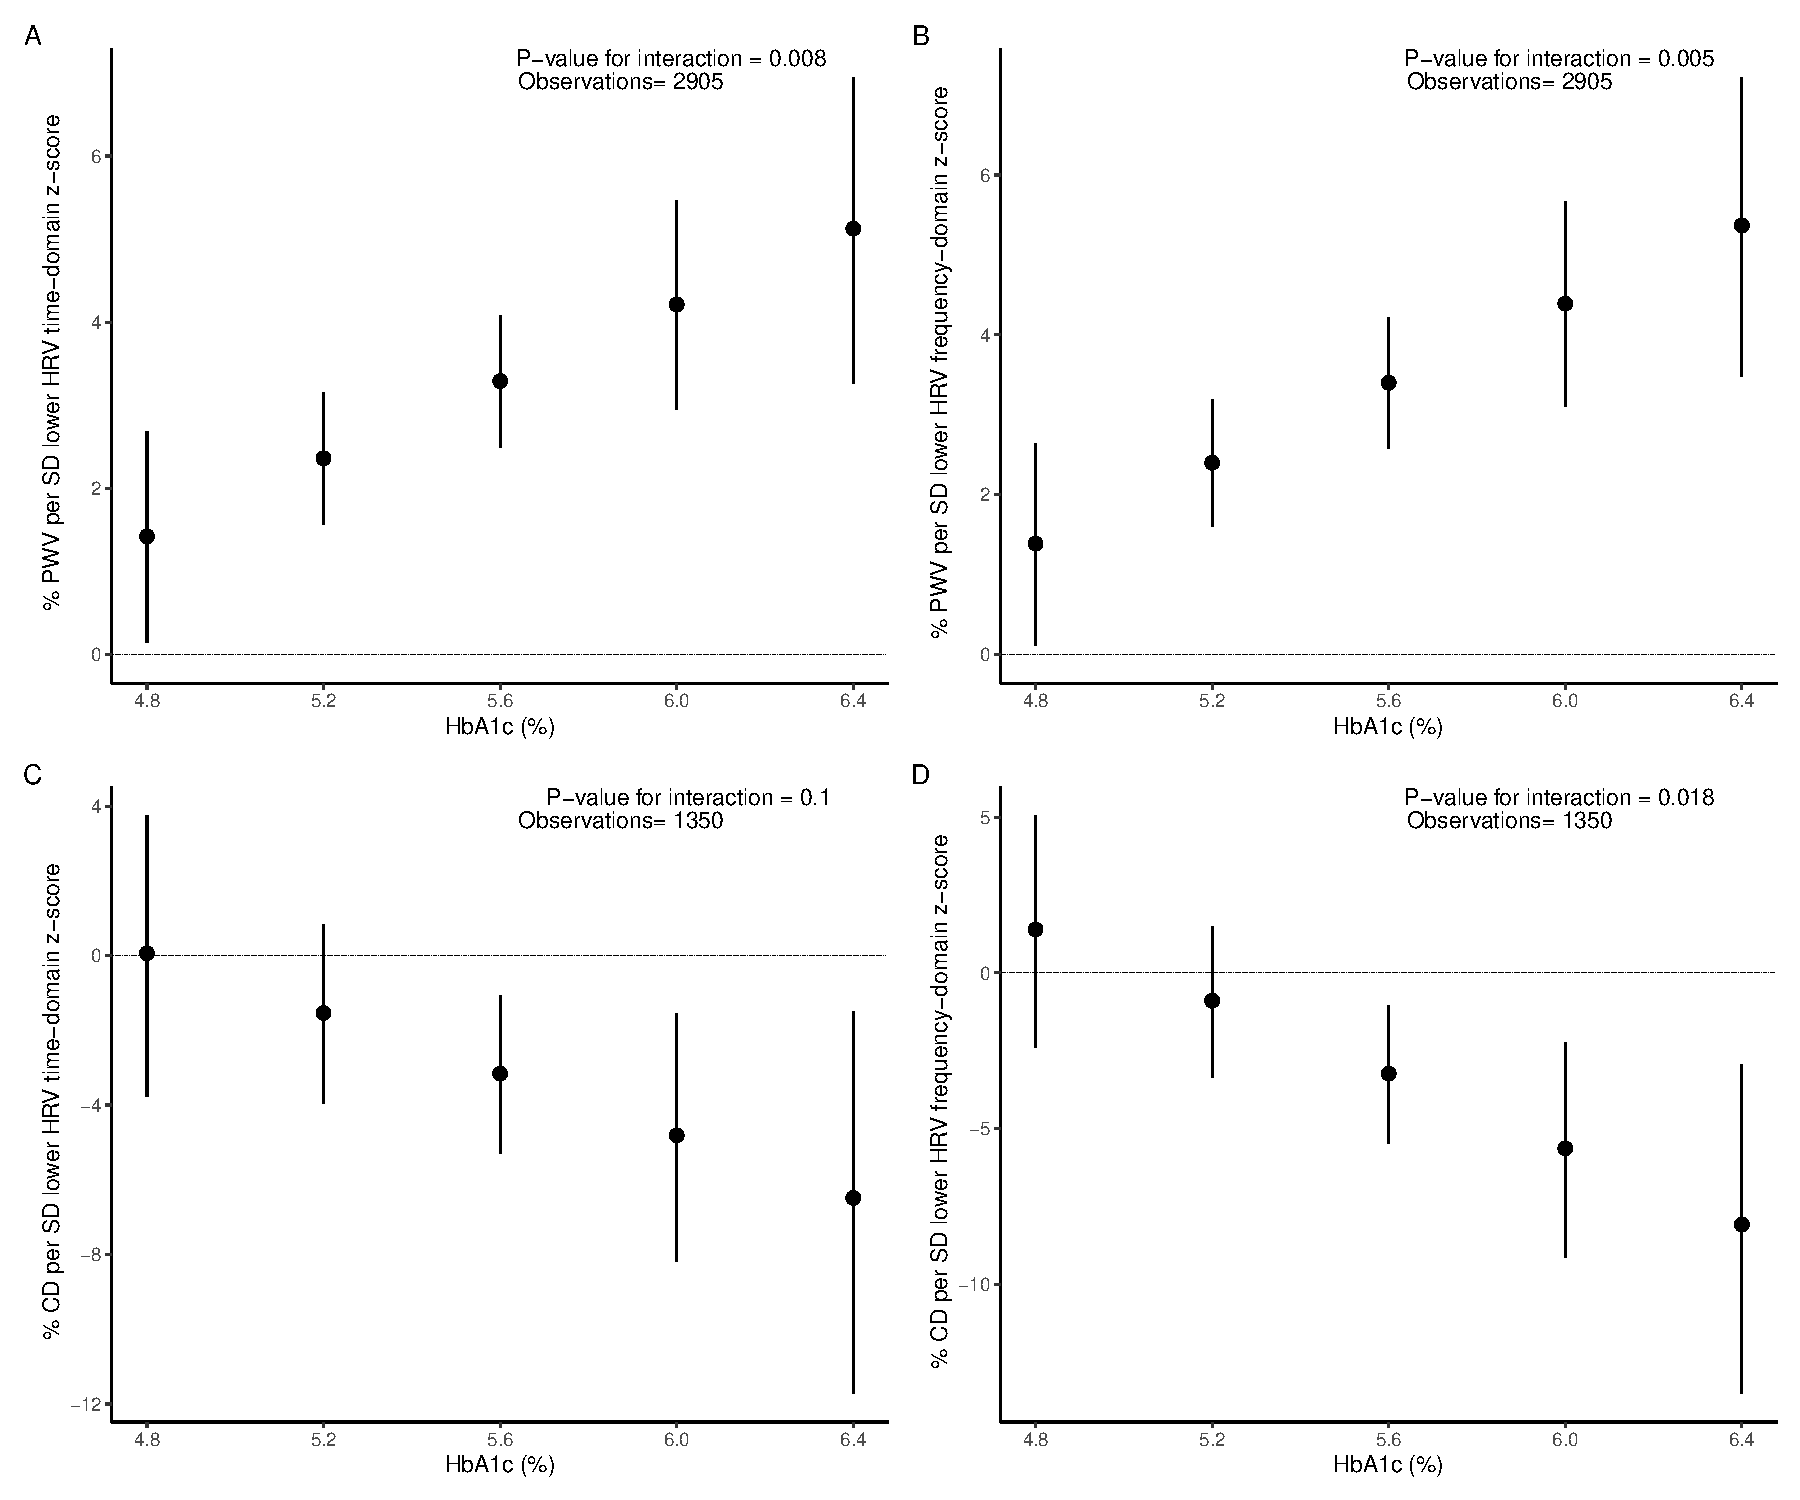
\includegraphics[width=4in,height=\textheight]{images/em_hba1c.pdf}

\hypertarget{study-ii-1}{%
\section{Study II}\label{study-ii-1}}

\hypertarget{descriptive-1}{%
\subsection{Descriptive}\label{descriptive-1}}

In ADDITION-PRO population consisted of 1,627 participant with a least
48-hour HRV measures, while 1,432 had all hour represented with hourly
HRV and physical acceleration. The study population included different
tiers of diabetes risk: 154 individuals at low risk (9\%), 889 at high
risk (51\%), 314 with impaired fasting glucose (IFG) (18\%), 226 with
impaired glucose tolerance (IGT) (13\%), and 161 with both IFG and IGT
(9\%). We splitted SDNN into categories by very-low (SDNN\textless{} 100
ms), low (SDNN 100-120 ms), middle (SDNN 121-140 ms), high (SDNN 141-160
ms) and very-high (SDNN \textgreater160 ms).

Participants in the lowest SDNN group (\textless100 ms) were older (67.4
± 6.9 years), had higher BMI (28.1 ± 5.4), HbA1c (5.9 ± 0.9),
triglycerides (1.5 ± 0.9 mmol/L), and resting heart rate (67.8 ± 5.7
bpm), were more likely to use anti-hypertensive medication (61\%), and
had lower physical activity energy expenditure (46.8 ± 24.0 kJ/day)
compared to those with higher SDNN levels.

\begin{table}
\centering
\resizebox{\linewidth}{!}{
\begin{tabular}{l|l|l|l|l|l|l}
\hline
Characteristic
 & Overall, N = 1,625
 & <100, N = 148
 & 100-120, N = 312
 & 120-140, N = 457
 & 140-160, N = 346
 & >160, N = 362
\\
\hline
sex &  &  &  &  &  & \\
\hline
Men & 866 (53\%) & 68 (46\%) & 148 (47\%) & 206 (45\%) & 203 (59\%) & 241 (67\%)\\
\hline
Women & 759 (47\%) & 80 (54\%) & 164 (53\%) & 251 (55\%) & 143 (41\%) & 121 (33\%)\\
\hline
Age (years) & 65.9 (6.8) & 67.4 (6.9) & 65.7 (6.9) & 66.0 (6.7) & 65.5 (6.6) & 66.0 (7.0)\\
\hline
Physical activity energy expenditure (KJ / day) & 53.1 (25.1) & 46.8 (24.0) & 49.4 (21.0) & 50.7 (21.5) & 57.6 (27.2) & 57.5 (29.2)\\
\hline
Alcohol consumption (units per week) & 9.2 (9.5) & 11.3 (10.8) & 10.2 (11.3) & 8.9 (8.5) & 8.5 (9.2) & 8.7 (8.2)\\
\hline
Smoking status &  &  &  &  &  & \\
\hline
1 & 263 (16\%) & 40 (28\%) & 70 (23\%) & 65 (14\%) & 41 (12\%) & 47 (13\%)\\
\hline
2 & 750 (47\%) & 58 (40\%) & 145 (47\%) & 214 (47\%) & 162 (47\%) & 171 (48\%)\\
\hline
3 & 598 (37\%) & 47 (32\%) & 95 (31\%) & 174 (38\%) & 140 (41\%) & 142 (39\%)\\
\hline
BMI (kg/m² & 27.7 (4.7) & 28.1 (5.4) & 28.2 (4.6) & 28.0 (4.7) & 27.7 (4.9) & 26.9 (4.2)\\
\hline
Waist circumference (cm) & 96.7 (13.4) & 98.0 (14.9) & 98.2 (13.2) & 96.7 (13.6) & 96.7 (13.1) & 94.8 (12.5)\\
\hline
Systolic blood pressure (mmHg) & 133.7 (17.3) & 134.2 (16.3) & 133.7 (17.6) & 133.5 (17.8) & 133.4 (16.9) & 133.8 (17.5)\\
\hline
Diastolic blood pressure (mmHg) & 81.9 (10.4) & 83.8 (10.1) & 82.7 (10.2) & 81.7 (10.6) & 82.1 (10.2) & 80.6 (10.3)\\
\hline
Pulse rate (bpm) & 67.4 (10.9) & 77.7 (11.2) & 72.6 (9.3) & 67.9 (9.3) & 65.3 (9.3) & 60.0 (9.8)\\
\hline
HbA1c (\%) & 5.8 (0.5) & 5.9 (0.9) & 5.9 (0.6) & 5.8 (0.5) & 5.7 (0.4) & 5.7 (0.4)\\
\hline
Triglycerides (mmol/L) & 1.3 (0.7) & 1.5 (0.9) & 1.4 (0.7) & 1.3 (0.6) & 1.2 (0.7) & 1.1 (0.6)\\
\hline
Total cholesterol (mmol/L) & 5.4 (1.1) & 5.2 (1.0) & 5.4 (1.2) & 5.4 (1.1) & 5.4 (1.0) & 5.4 (1.0)\\
\hline
HDL cholesterol (mmol/L) & 1.6 (0.4) & 1.6 (0.4) & 1.5 (0.5) & 1.6 (0.4) & 1.6 (0.4) & 1.6 (0.4)\\
\hline
LDL cholesterol (mmol/L) & 3.2 (1.0) & 3.0 (1.0) & 3.2 (1.1) & 3.2 (1.0) & 3.3 (0.9) & 3.3 (0.9)\\
\hline
Urine albumin-creatine ratio (mg/g) & 25.9 (132.8) & 36.4 (105.9) & 47.9 (275.1) & 19.6 (48.2) & 19.4 (67.7) & 16.4 (36.3)\\
\hline
vo2max & 26.6 (7.8) & 24.8 (7.5) & 24.8 (7.5) & 26.1 (6.8) & 27.0 (8.0) & 28.7 (8.7)\\
\hline
rest\_hr & 57.3 (7.3) & 67.8 (5.7) & 63.3 (5.0) & 58.4 (4.5) & 55.0 (4.2) & 49.8 (4.9)\\
\hline
med\_any\_anti\_hypertensive & 753 (47\%) & 88 (61\%) & 149 (48\%) & 216 (47\%) & 147 (43\%) & 153 (43\%)\\
\hline
\end{tabular}}
\end{table}

\hypertarget{multiday-hrv-and-mace-heart-failure-and-all-cause-mortality.}{%
\subsection{multiday HRV and MACE, heart failure, and all-cause
mortality.}\label{multiday-hrv-and-mace-heart-failure-and-all-cause-mortality.}}

The mean multiday SDNN was 139.0 (32.3) ms, and the mean heart rate was
73.5 (9.1) bpm. In the fully adjusted model, SDNN per SD was associated
with a lower incidence rate ratio (IRR) for MACE 0.82 (CI: 0.69; 0.97),
heart failure 0.76 (CI: 0.58; 0.99), and mortality rate ratio of 0.79
(CI: 0.66; 0.94). When we pre-adjusted for resting heart rate, the
proportion of the association explained between HRV and MACE, HF, and
all-cause mortality was 14\%, 25\%, and 19\%, respectively. We included
knots in the model, which showed that the risk increased when SDNN fell
below 120 to 110 ms (approximately below the 20th percentile),
suggesting a potential cut-off point for higher risk. We therefore
calculated the incidence rate (IR) at SDNN levels of 100 ms, 120 ms, and
160 ms, respectively, and plotted these as a function of age. :::
\{.center\}
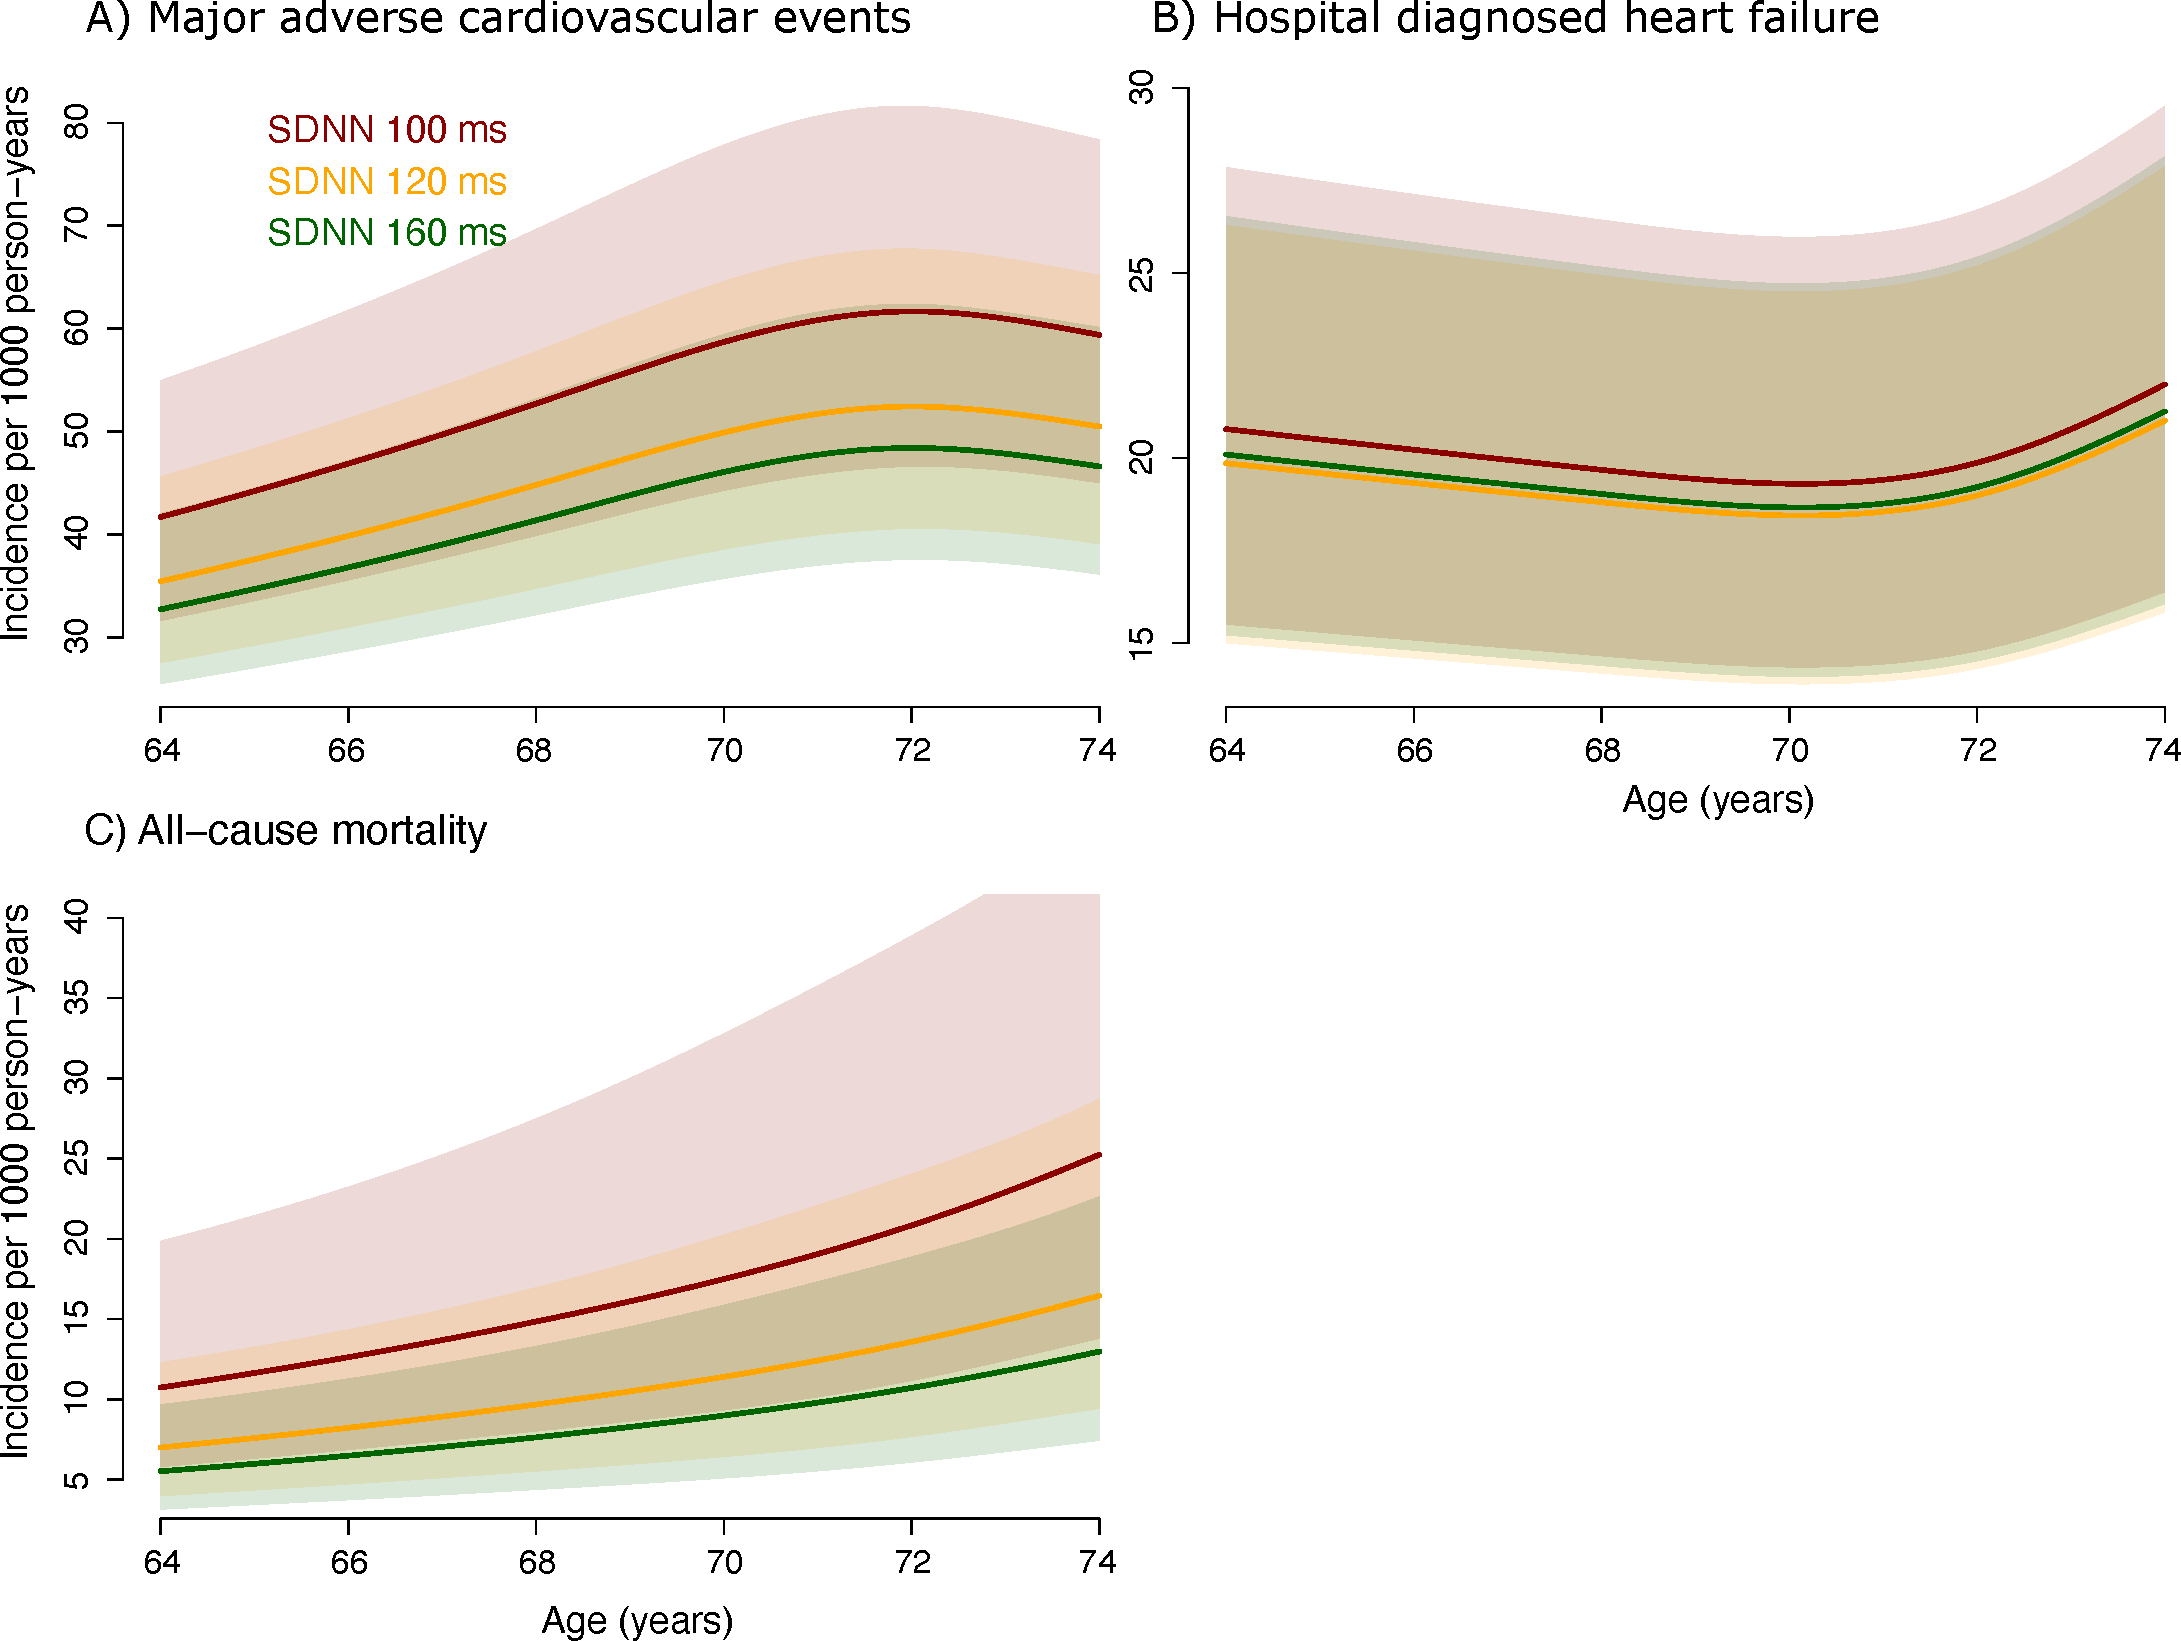
\includegraphics[width=4in,height=\textheight]{images/addition_pro_hrv_ir_mace.pdf}
:::

At age 65, the IR per 1000 person-years for MACE was 44.2 (CI: 33.5;
58.3) at SDNN = 100 ms, which was higher than the rates observed at SDNN
= 120 ms (IR: 37.6 {[}CI: 29.2; 48.3{]}) and SDNN = 160 ms (IR: 34.7
{[}CI: 27.0; 44.5{]}) (Figure xA). The IR became higher with age,
reaching its peak at age 72. For heart failure at age 65, the IR was
20.5 (CI: 15.3; 27.5) at SDNN = 100 ms, slightly higher than at SDNN =
120 ms (IR: 19.6 {[}CI: 14.8; 25.9{]}) and SDNN = 160 ms (IR: 19.8
{[}CI: 15.0; 26.2{]}) (Figure xB). The IR remained stable until age 70,
after which it became higher. For all-cause mortality at age 65, the IR
was 11.6 (CI: 6.3; 21.4) at SDNN = 100 ms, higher than at SDNN = 120 ms
(IR: 7.6 {[}CI: 4.3; 13.3{]}) and SDNN = 160 ms (IR: 6.0 {[}CI: 3.4;
10.4{]}) (Figure xC). The IR for all-cause mortality became higher with
age.

\hypertarget{hourly-hrv-and-mace-heart-failure-and-all-cause-mortality.}{%
\subsection{Hourly HRV and MACE, heart failure, and all-cause
mortality.}\label{hourly-hrv-and-mace-heart-failure-and-all-cause-mortality.}}

From the hourly recordings, we observed a clear periodicity in SDNN,
mean heart rate (HR), sleep patterns, and physical acceleration. SDNN
increased from 5--6 AM, peaking at 8--9 AM {[}mean (SD){]}, followed by
a gradual decline, reaching its lowest point around 1 AM the next day
{[}mean SDNN (SD){]}. A similar circadian pattern was observed in heart
rate, though its peak occurred two hour later at 10--11 AM. After
peaking, heart rate remained stable throughout the afternoon before
gradually decreasing. {[}Add IRR results{]}

\begin{figure}

{\centering 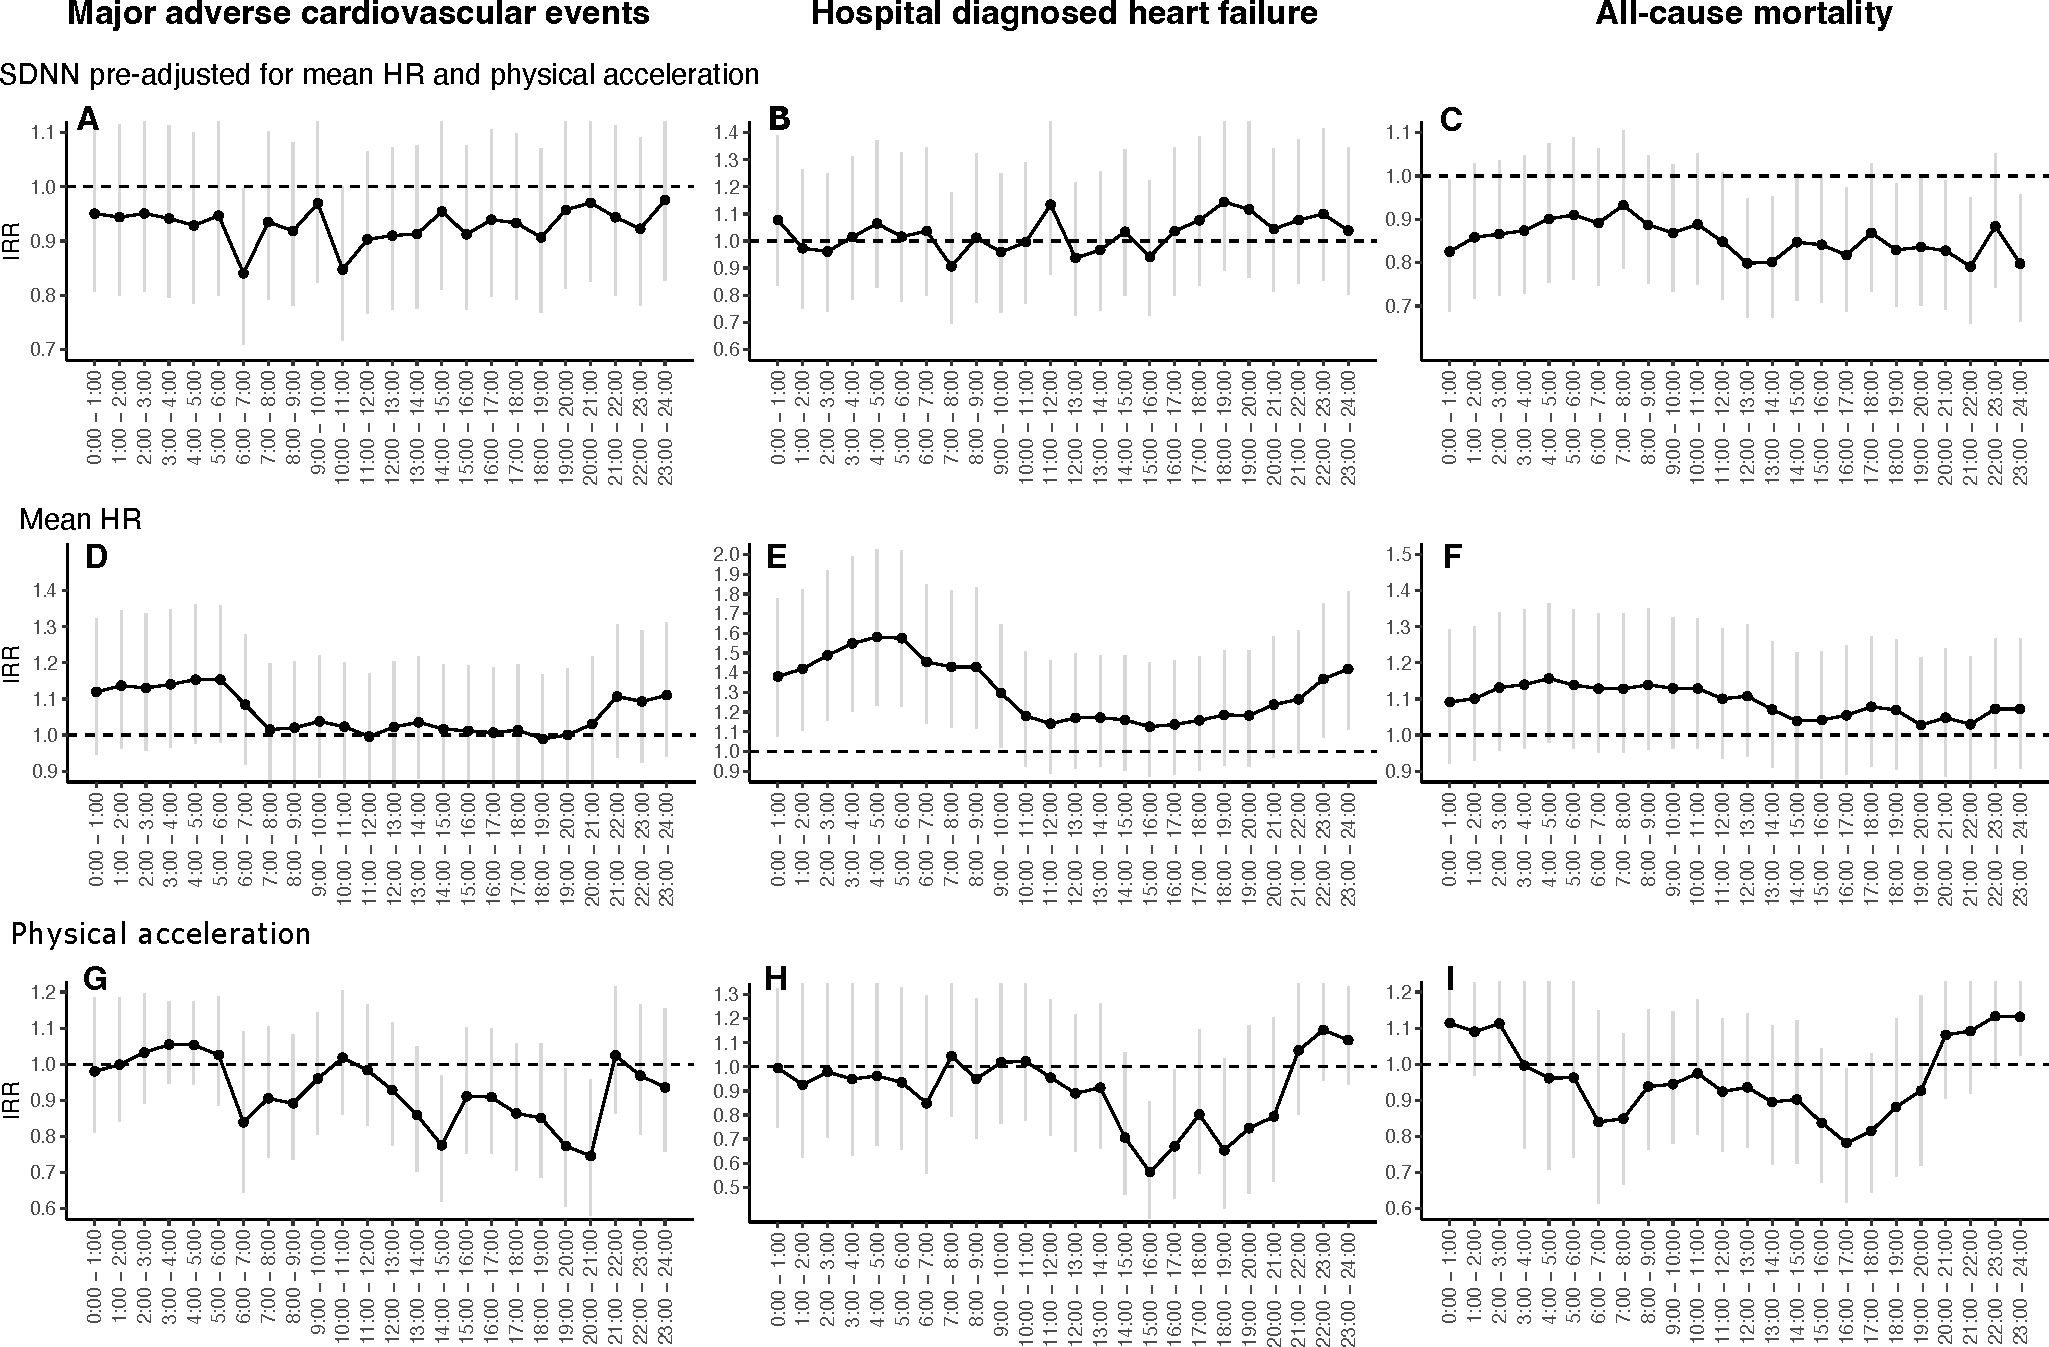
\includegraphics[width=7in,height=\textheight]{images/figure_ADD_PRO_risk_by_hour.pdf}

}

\caption{Hourly SDNN levels (100 ms, 120 ms, 160 ms) by age-specific
incidence rates for A) major adverse cardiovascular events, B) heart
failure, and C) all-cause mortality. Figure adapted from {[}authors{]}.
---. (Paper II, appendix)}

\end{figure}

\hypertarget{study-iii-1}{%
\section{Study III}\label{study-iii-1}}

\hypertarget{patients-characteristics}{%
\subsection{Patients characteristics}\label{patients-characteristics}}

In study III, 179 participants with type 2 had measures of NT-proBNP and
performed the CART test. CAN was present in 30\% (n = 54) of
participants (36\% among those with valid CAN measurements). Meanwhile,
24\% (n = 43) were unable to complete the CART assessment adequately,
primarily due to irregular heart rhythms (n = 8) or insufficient air
pressure during the Valsalva manoeuvre (n = 21). Compare to those
without CAN, the participants with CAN were more women (41 \% vs 33 \%),
were more sedentary (45\% vs 36\%), had a higher proportion with prior
major CVD (41\% vs 20\%) and declined eGFR (\textless{} 60) (36\% vs
22\%), higher levels of triglyceride (median 2.05 mmol/L vs 1.95 mmol/
L), were slightly older (median 62 years vs 61 years), had longer
duration of type 2 diabetes (median 19 years vs 15 years), and higher
use SGTL2-inhibitors (65\% vs 60\%) but lower use of GLP-1 RA (63\% vs
70\%). No other difference in clinical characteristic was observed.

\hypertarget{relationship-between-can-and-elevated-nt-probnp}{%
\subsection{Relationship between CAN and elevated
NT-proBNP}\label{relationship-between-can-and-elevated-nt-probnp}}

A greater proportion of individuals with CAN exhibited elevated
NT-proBNP levels (\textgreater125 pg/ml) (51.9\%, n=52/78) compared to
those without CAN (23.2\%, n=26/112). The fully adjusted odds ratio (OR)
for elevated NT-proBNP in individuals with CAN was 5.69 (95\% CI: 1.95,
18.49) relative to those without CAN. Among the cardiovascular autonomic
reflex tests (CART), the Valsalva maneuver demonstrated the strongest
association with NT-proBNP (OR 9.00, 95\% CI: 2.88, 33.09; n=51/75),
followed by deep breathing (OR 3.30, 95\% CI: 1.17, 9.77; n=33/133) and
orthostatic hypertension (OR 4.04, 95\% CI: 1.27, 13.77; n=24/146). No
significant association was identified for the lying-to-standing test
(OR 0.80, 95\% CI: 0.32, 1.97; n=54/108). After imputing missing CART
data, the OR for CAN in relation to elevated NT-proBNP declined to 2.94
(95\% CI: 1.37, 6.56). Sensitivity analyses, which excluded participants
using beta-blockers or those with a history of CVD, resulted in a
smaller sample size and wider confidence intervals, though the overall
association remained unchanged. {[}Add NYHA and WATCH-DM modification{]}

\begin{figure}

\begin{minipage}[t]{\linewidth}

{\centering 

\raisebox{-\height}{

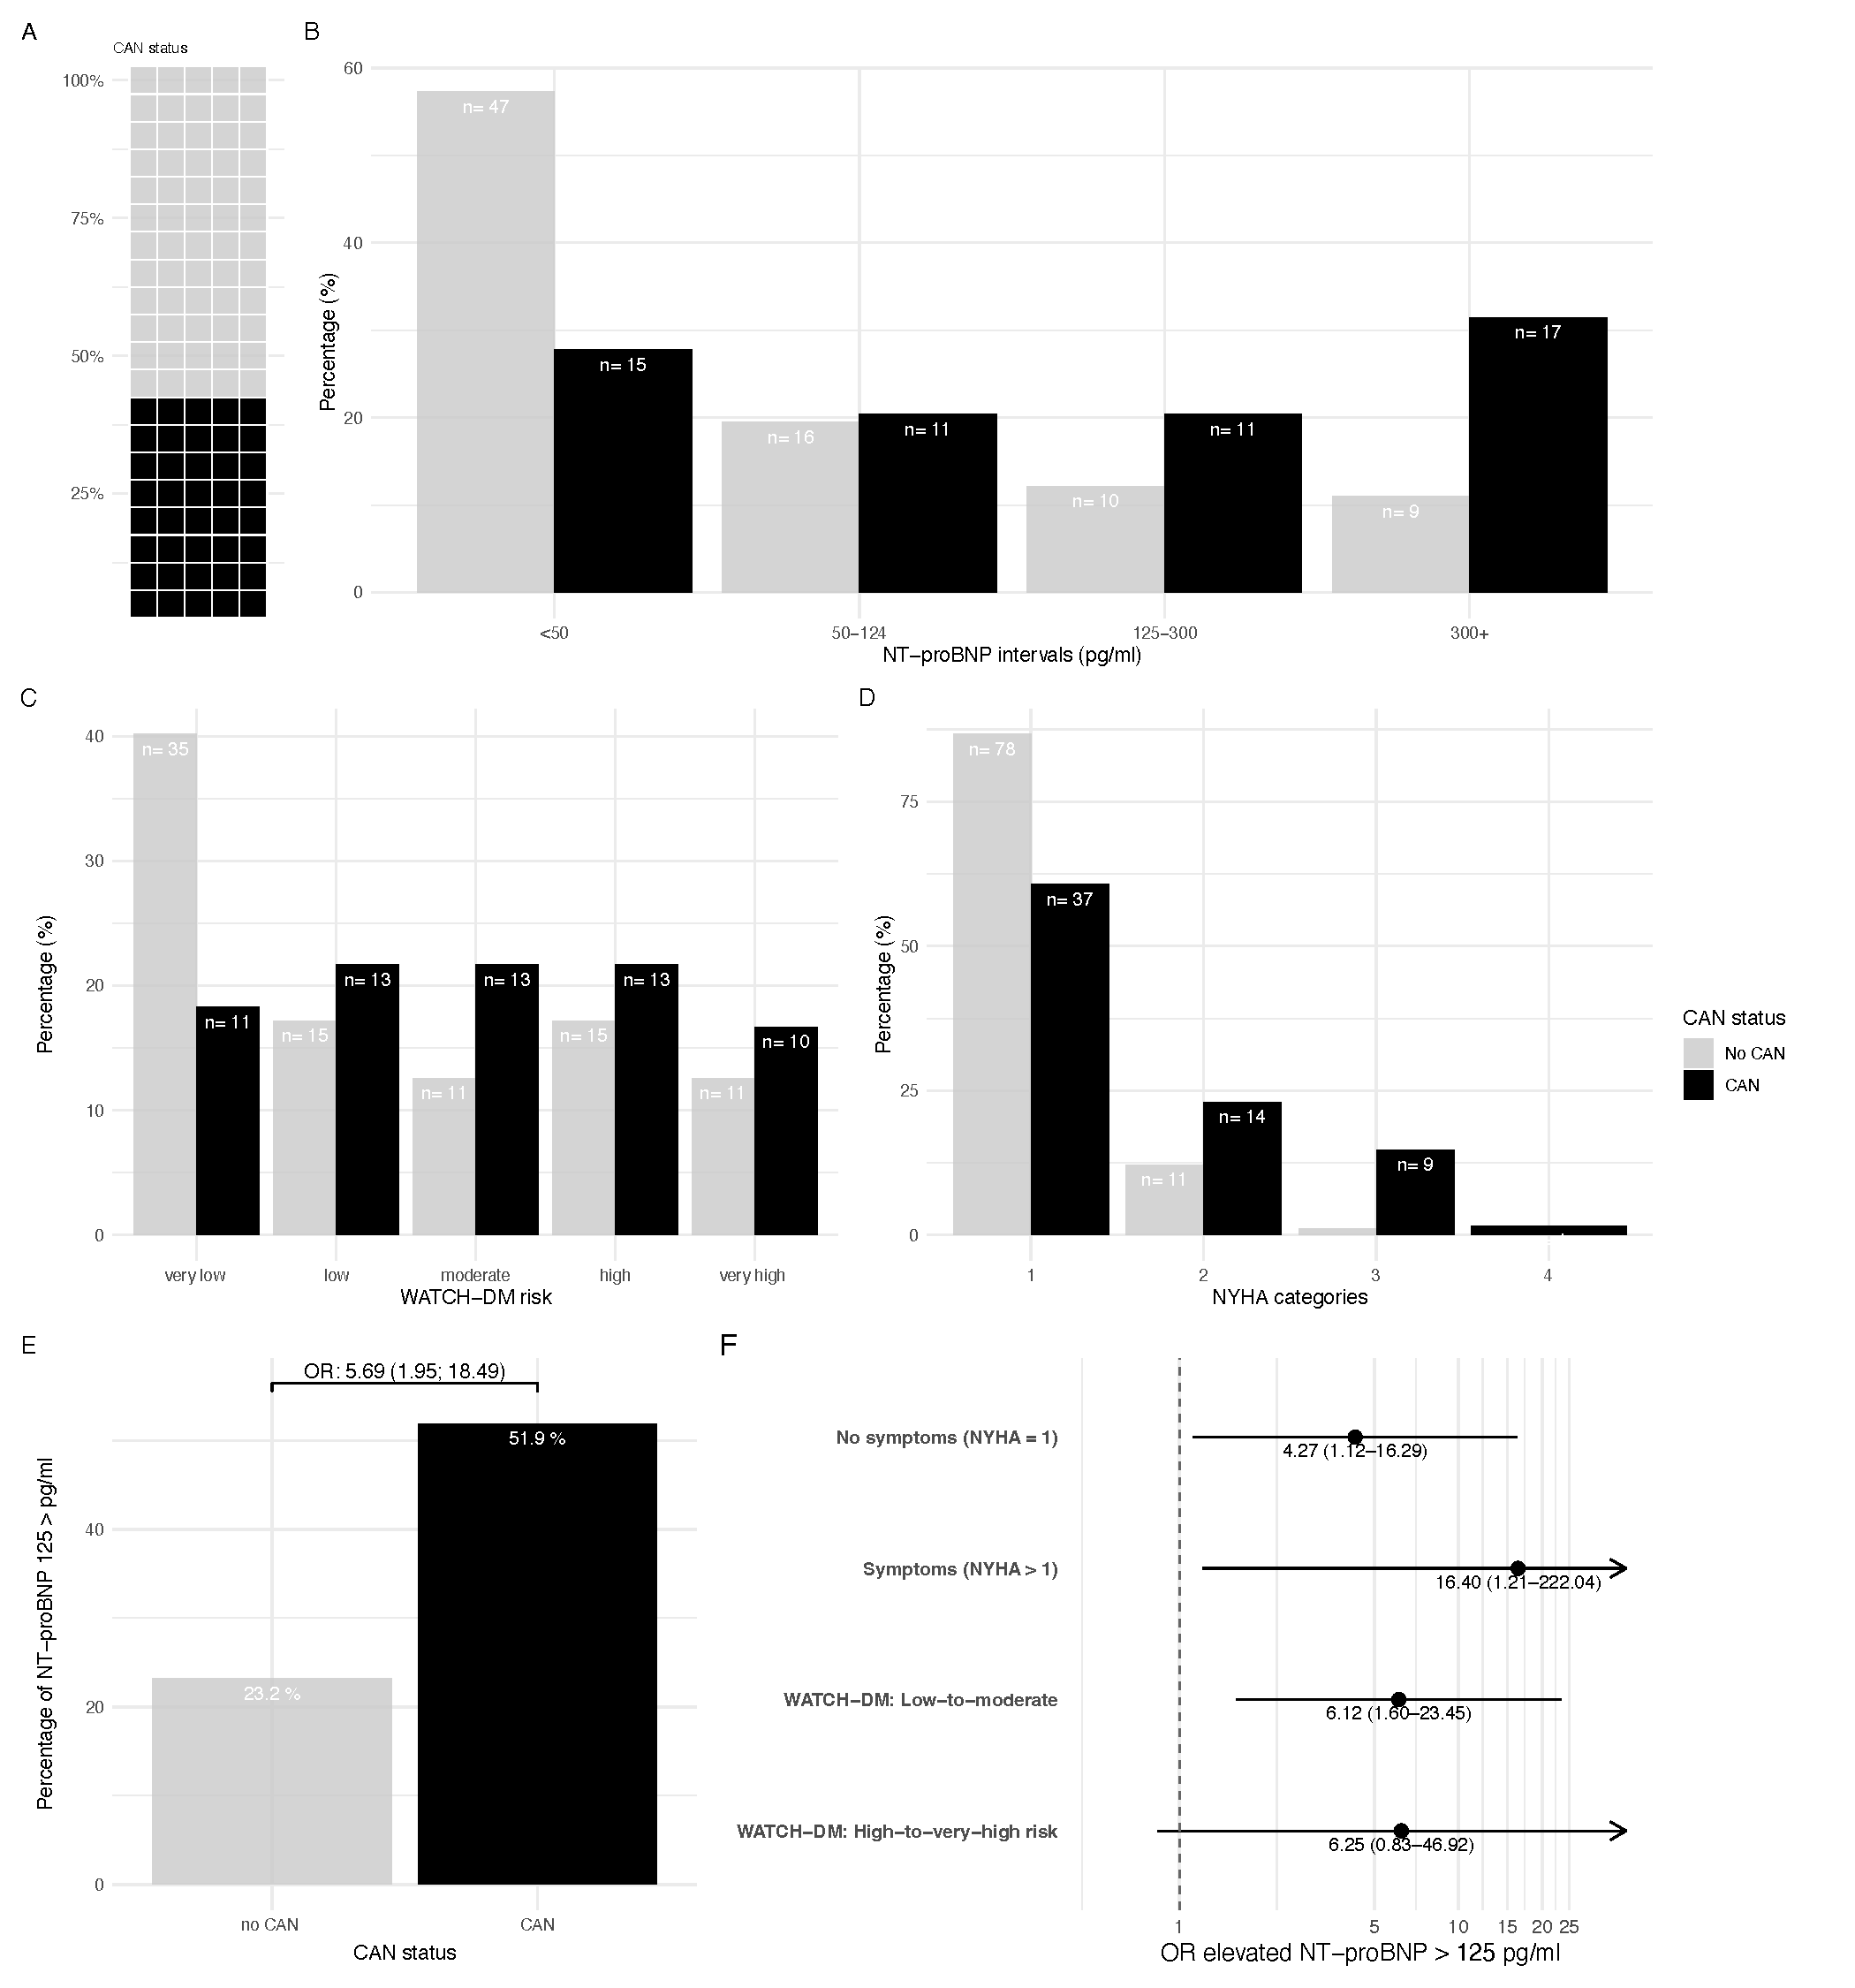
\includegraphics{images/heart_failure_distribution_can_figure_2.pdf}

}

\caption{Relationship betweeen CAN and indicators for heart failure.
Figure from {[}authors{]}. Cardiovascular autonomic neuropathy and
indices of heart failure in type 2 diabetes: The CANCAN Study. (Paper
III, appendix)}

}

\end{minipage}%

\end{figure}

\begin{verbatim}



`<!-- quarto-file-metadata: eyJyZXNvdXJjZURpciI6Ii4ifQ== -->`{=html}

```{=html}
<!-- quarto-file-metadata: eyJyZXNvdXJjZURpciI6Ii4iLCJib29rSXRlbVR5cGUiOiJjaGFwdGVyIiwiYm9va0l0ZW1OdW1iZXIiOjYsImJvb2tJdGVtRmlsZSI6IjYtZGlzY3Vzc2lvbi5xbWQiLCJib29rSXRlbURlcHRoIjowfQ== -->
\end{verbatim}

\bookmarksetup{startatroot}

\hypertarget{discussion-needs-to-be-fine-tuned}{%
\chapter{Discussion {[}needs to be
fine-tuned{]}}\label{discussion-needs-to-be-fine-tuned}}

\hypertarget{strength-and-limitation}{%
\section{Strength and limitation}\label{strength-and-limitation}}

\hypertarget{study-design}{%
\subsection{Study design}\label{study-design}}

\emph{Cross-sectional design}

Studies I and III are based on cross-sectional data, with exposure and
outcome measured within a three-month period. The main limitation of
this design is that it does not allow us to determine whether the
exposure led to the outcome or vice versa. As a result, we cannot
establish temporarily or confirm whether changes in the outcome were
caused by the exposure. However, based on prior evidence, we assume the
direction of the studies based on physiological knowledge and in vivo
studies. In Study I, we based our direction of the association based on
longitudinal association based on data from Whitehall II study, showing
steeper decrease in short-term HRV are associated with subsequent higher
levels of cf-PWV\textsuperscript{24}. Moreover, {[}insert in vivo
studies{]}. In Study II, we attempted to mimic temporarily by glucose
metabolism, in individuals with type 2 diabetes and without known type 2
diabetes, instead of time, which shows deterioration of glucose
metabolism increases the size of the association. The strength of study
I, is that sample size is large, making our results more generalisable
to wider populations across statuses of glucose metabolism.

In study III, our study design are more focused on the clinical
diagnosis of CAN and presence of heart failure. This the question are
more focused on clinical utilization of CAN in detecting type 2 diabetes
patients who early progress towards heart failure, and thus the
aetiological question remain for other study design. Indeed, whether
cardiac function progressively worsens due to the etiological mechanisms
of CAN remains to be fully established. If confirmed, this would
underscore the relevance of CAN as a preclinical marker for early
progression to heart failure, one that may be effective to target in
efforts to prevent or delay the development of overt heart failure.

\emph{Longitudinal design}

A major strength of study II is its longitudinal design, where HRV was
measured at baseline and outcomes were captured prospectively through
national registries. This temporal structure ensures that the exposure
(HRV) clearly preceded the outcome, reducing the risk of reverse
causation. Although repeated measurements of HRV over time would provide
more detailed insights into autonomic function dynamics, the prospective
design still allows for stronger inference of directionality than
cross-sectional studies. Furthermore, the use of high-quality registry
data for outcome ascertainment ensures complete follow-up and minimizes
loss to follow-up bias.

Based on our studies, we demonstrate first steps in relationship between
cardiovascular autonomic function, measured by, HRV or CART, we can only
establish an association and cannot conclude with certainty that
improvements in HRV measures lead to a reduction in cardiovascular risk.
Therefore, we cannot ascertain causal effect based on our findings, and
more causal focused methods are needed. Mendelian randomization, which
uses genetic instruments for exposure, could help address this causal
question. Furthermore, structured mediation analysis involving
modification, e.g.~by medication or lifestyle, would improve HRV or CART
leads to reduction in cardiovascular risk, using data from intervention
studies.

\hypertarget{intern-validity}{%
\subsection{Intern validity}\label{intern-validity}}

In this project, we aimed to assess cardiovascular autonomic function
both in free-living conditions and in response to standardized test
procedures during clinical visits. Additionally, we used dynamic
measurements to evaluate arterial stiffness locally and by velocity and
biomarker assessments to determine the presence of heart failure. In
this section, I will discuss the validity of 24-hour, week-long, and
hourly HRV measurements, as well as the standardized tests of CAN.
Furthermore, I will address the validity of the included outcomes. I
will as well discuss using the strength and limitation of using MACE as
an time to event outcome.

\hypertarget{long-term-hrv-24-hours-as-measurement-for-autonomic-function}{%
\subsubsection{Long-term HRV (\textgreater24 hours) as measurement for
autonomic
function}\label{long-term-hrv-24-hours-as-measurement-for-autonomic-function}}

{[}Actiheart and Holter monitor{]}

HRV has been applied across several research domains. For example, in
psychology as a marker of mental stress, in exercise physiology as an
indicator of recovery, in cardiovascular research as a marker of
autonomic dysfunction as a consequence to cardiac complications, and in
diabetes research as a marker of autonomic neuropathy. In the context of
this project, which focuses on long-term HRV in diabetes and
cardiovascular research, it is important to acknowledge that the
autonomic nervous function we aim to assess, may also be influenced by
behavioral factors such as physical activity, sleep, meal timing,
emotions, smoking, caffeine intake, alcohol consumption, use of
medication, and prior cardiovascular complications which can potentially
masking or mimicking underlying physiological dysfunction during
recordings. Therefore, reduced long-term HRV cannot be interpreted
solely as a marker of autonomic function. Moreover, HRV is also
influenced by lifestyle patterns over time, making it sensitive not only
to acute behaviors but also to long-term habits that affect autonomic
balance. In study II, we observed that the lower ranges of HRV had both
lower habitual physical activity and lower VO\textsubscript{2} max,
suggesting that lower HRV reflects more sedentary lifestyle and lower
cardiorespiratory fitness.

In study I and II, we strived to account for habitual physical activity,
while in study II, we also accounted hourly HRV for physical movement
during the recording to test the influence of concurrent physical
activity. However, further studies are need to understand how lifestyle
patterns affect the long-term recording the subsequent day, to
understand the behavioral component in long-term HRV. In study I and II,
we also excluded participants with prior CVD to ensure that in order to
keep etiological order between autonomic dysfunction and the outcome of
cardiovascular complication.

Anti-hypertensive medications, especially beta-blockers, are known to
increase HRV in randomized controlled trials\textsuperscript{25}.
However, in cohort studies, participants using anti-hypertensives
generally show lower HRV, likely reflecting their higher burden of
cardiovascular complications {[}ref{]}. Because beta-blockers target the
autonomic nervous system, some anti-hypertensive medications may
introduce bias in HRV measurements, as they interfere with the autonomic
function we aim to assess. In the sensitivity analysis in study I and
III, without participants on anti-hypertensive treatment, the estimates
did not materially change, thus we included the population and adjusted
for medication in the full model

HRV levels are influenced by heart rate as lower resting heart rate
allows higher variability. In study I, we chose not to adjust for heart
rate in our models, as doing so could introduce issues of
multicollinearity. Additionally, elevated heart rate is driven by
increased sympathetic activity and may act as a mediator in the pathway
leading to arterial stiffness. Our use of full-day recordings captures
HRV during both rest and activity, providing a robust representation of
autonomic function over the course of a typical day. In contrast, heart
rate correction may be more relevant for short-term recordings of HRV,
where standardized conditions can be affected by random influences such
as time of day, smoking, or caffeine intake, which have been relevant
for study III if we had included HRV measures. In Study II, we included
HRV measures pre-adjusted for heart rate, which accounted for part of
the observed associations, particularly with heart failure and all-cause
mortality, but to a lesser extent for ischemic-related CVD events.
Similar trends were observed in the hourly associations, where heart
rate pre-adjustment had comparable effects on the outcomes.

{[}When HRV is analyzed in shorter segments (e.g., hourly or in 5-minute
intervals), measures like RMSSD, pNN50, and HF appear to offer new
insights into autonomic function and its relevance in diabetes and CVD,
e.g during night-time {[}\textsuperscript{26}{]}\textsuperscript{27}.
SDANN and SDNNi aim to reduce the impact of short-term variability, such
as that caused by physical activity, by calculating either the standard
deviation of 5-minute segment mean IBI (SDANN) or the mean of standard
deviations across 5-minute segments (SDNNi). {[}include lower-frequency
points{]}. This helps smooth out transient fluctuations and better
capture long-term autonomic modulation. Thus, behavioral patterns pose a
limitation in physiological research aiming to disentangle the causal
pathways between autonomic dysfunction and CVD when using long-term HRV
measures. These patterns likely introduce high variability between
observations that is not attributable to autonomic function itself.{]}

{[}{[}HRV is just a proxy for heart rate, controversy?{]} - HRV is just
a proxy for heart rate - direct sympathetic activity at the location,
but a proxy from heart rate signals.{]}

\hypertarget{cardiovascular-autonomic-reflex-test}{%
\subsubsection{Cardiovascular autonomic reflex
test}\label{cardiovascular-autonomic-reflex-test}}

CART offers a practical approach to screening for autonomic dysfunction,
as the test has been shown to be reliable\textsuperscript{28}. While
some CART indices may be influenced by the time of day or recent
physical activity, these effects are generally considered minimal.
Additionally, no impact of caffeine intake on the reference age-based
formular has been observed\textsuperscript{29}.

\hypertarget{measures-of-cardiovascular-risk}{%
\subsubsection{Measures of cardiovascular
risk}\label{measures-of-cardiovascular-risk}}

{[} Arterial stiffness - NT-proBNP - MACE limitation in aetiological
research - Non-specific heart failure and MI and stroke and death - HRV
stronger link with MI or stroke - Perspective: decreasing number of
events with prolonging time-to-event - Clinical trail moved to high risk
population in lower-income countries (South America) - Challenge for
coming observational cohorts (need to increase sample size) {[}The
Problem With Composite End Points in Cardiovascular Studies The Story of
Major Adverse Cardiac Events and Percutaneous Coronary
Intervention{]}{]}

\hypertarget{external-validity}{%
\subsection{External validity}\label{external-validity}}

\hypertarget{selection-bias}{%
\subsubsection{Selection bias}\label{selection-bias}}

\textbf{The Maastricht Study}

In Study I, participants were recruited using different strategies, with
a focus on enrolling individuals with type 2 diabetes to ensure
sufficient statistical power in this group. Recruitment was conducted
through mass media campaigns, municipal registries, and the regional
Diabetes Patient Registry via mailings. Thus, participation depended on
individuals' awareness of the campaigns and their willingness to attend.
Patients with type 2 diabetes were actively targeted with additional
mail invitations to encourage participation.

\textbf{ADDITION-PRO}

In Study II, participants were recruited through a step-wise screening
procedure. First, they were selected based on a risk score by
self-administrated questionnaire sent by mail , followed by HbA1c or
random glucose measurements. These procedures introduce different steps
for selection bias as people have both to receive and sent a filled
questionnaire, followed by a visit for blood testing if their risk score
was high\textsuperscript{30}.

First, the population consists of participants who responded to the
screening questionnaire and those at higher risk who underwent further
blood measurements. Second, the questionnaire itself selects
participants based on a risk score developed to identify individuals
with type 2 diabetes, while prediabetes identification was based on
further measurement on the basis of HbA1c measurements. Certain risk
factors, such as age and hypertension, contribute to higher risk by
influencing the risk score, and thus may lead to high representation of
these groups.

Hence, selection bias arises from both participation in the risk score
assessment and follow-up attendance in ADDITION, as well as from the
instruments used to identify risk, the Inter-99 risk score, HbA1c, and
random blood glucose measurements. Healthier people are more attentive
in screening and cohort studies {[}ref.{]}.

\textbf{CANCAN}

In Denmark, patients with type 2 diabetes are referred to diabetes
specialists at outpatient clinics when their general practitioner is
unable to stabilize their diabetes care. As a result, CANCAN
participants represent a higher-risk group in Danish diabetes patients,
where more stable patients remain under general practitioner care.
Consequently, the prevalence of heart failure indicators and CAN is
likely higher in this selected group. The strength of the CANCAN
sampling strategy in outpatient clinics is that patients were referred
to an endocrinologist and attended their consultations. The additional
study examination did not require extra transport or appointments but
only involved additional time during their visit, with the option of
receiving feedback on continuous glucose monitoring.

Overall in this project, the selection bias span across different
aspects. In Study I-II, healthier and more health-conscious individuals
tend to participate in cohort studies, potentially introducing selection
bias. In contrast, attendance in the study III was more successful, as
participation was optimized by scheduling study assessments during
routine consultations. In epidemiology, we aim to match the source
population with our target population. However, limitations due to
self-selection in participation arise. Consequently, this can affect the
results, as participants may be healthier and better using health care
services, leading to less contrast between determinants and outcomes in
our etiological analysis. We suspect that one explanation for the lack
of a stepwise increase in the association between HRV and arterial
stiffness across prediabetes and type 2 diabetes in study II is that the
participants with type 2 diabetes represent a well-treated population.
Although, the included participants may be sufficient to demonstrate a
relationship, the magnitude of the association in groups with type 2
diabetes may be limited.

\hypertarget{generalisability}{%
\subsubsection{Generalisability}\label{generalisability}}

The generalizability of our findings can be discussed on two levels: the
extent to which the results apply to the general population within the
country and how they translate to populations with different ancestries
in other countries.

Studies II--III include individuals at high risk of diabetes and those
with type 2 diabetes. Therefore, the associations between cardiovascular
autonomic dysfunction and cardiovascular outcomes or surrogate
biomarkers extend to individuals with some degree of diabetes risk.
However, whether these associations hold in the general populations
remains uncertain. Study I suggests that the link between autonomic
dysfunction and cardiovascular risk, as measured by arterial stiffness,
is also present in individuals with normal glucose metabolism, though to
a lesser extent. This finding was further supported by replication in
the Whitehall II cohort, strengthening the generalizability of the
observed relationship\textsuperscript{24}.

The study populations in Studies II--III consist of individuals of
Nordic descent, while Study I represents a population of Western
European descent. Since the constellation of risk factors for diabetes
varies and may manifest differently in population with Asian, South
American, African, and other decent, and therefore our findings may not
be fully generalizable to these groups. This limitation affects the
applicability of the observed associations and their magnitudes to a
unknown degree. Further cohort studies including under-represented
populations are warranted. As we are studying diabetes risk, all
participants in the study were older adults aged 40 years and above.
Therefore, our findings are limited to this age group, and whether the
results extend to younger adults or children remains to be confirmed.
Overall, while our study has the strength of including individuals
across different levels of diabetes risk, some limitations in
generalizability remain, particularly to more diverse and younger
populations.

\hypertarget{discussion-of-results}{%
\section{Discussion of results}\label{discussion-of-results}}

The challenges of population of type 2 diabetes and the risk of
developing diabetes are addressed at multiple levels within the
healthcare system.

\begin{itemize}
\item
  Public health focuses on preventing diabetes and its complications
  across all age groups, from childhood to older adulthood.
\item
  Primary care, especially general practitioners, plays a central role
  in identifying individuals at risk of diabetes and cardiovascular
  disease. General practitioners also manage patients with uncomplicated
  type 2 diabetes.
\item
  Outpatient clinics, led by endocrinologists, are responsible for
  treating patients with more advanced stages of diabetes and for
  managing complex cases.
\end{itemize}

The aim of this thesis is to understand how cardiovascular autonomic
dysfunction and CAN affects the risk of cardiovascular disease across
stage of glucose metabolism. We included conditions such as heart
failure, stroke, and myocardial infarction, as well as subclinical
markers like carotid-femoral pulse wave velocity and carotid artery
distensibility. The thesis includes populations across from normal
glucose metabolism to type 2 diabetes and considers individuals engaged
at different levels of the healthcare system. This chapter discusses the
results and conclusions in relation to existing evidence and addresses
their clinical implications across the levels of the health care system.

To address this aim, we used three different cohorts that reflect
various levels of prevention and care. In Study I, we approached the
question from a public health perspective by using data from The
Maastricht Study including individuals aged 40 and above, representing
all stages from normal glucose metabolism to type 2 diabetes. In this
broader population, we demonstrated a link between lower 24-hour HRV and
cardiovascular risk, measured by arterial stiffness. This association
was modified by glucose metabolism, showing a stronger relationship in
individuals with prediabetes and type 2 diabetes.

This led to a focus on individuals at higher risk of developing
diabetes, using data from the ADDITION-PRO cohort. Individuals with
prediabetes may benefit from structured guidance in primary care to
prevent progression to type 2 diabetes and related complications such as
CVD. In study II, we showed in a population with prediabetes, that lower
multiday HRV was linked to higher risk of CVD, heart failure and
all-cause mortality.

A key challenge in managing type 2 diabetes lies in the complexity of
clinical decision-making, which is often applied uniformly across a
heterogeneous patient population. As the duration of diabetes increases,
the disease typically progresses, leading to a higher prevalence of both
microvascular and macrovascular complications. This raises the need to
early identify subgroups of individuals who may benefit from more
structured and personalized treatment strategies based on their risk
profile. However, to support such an approach, reliable and standardized
tools are required to accurately detect and classify high-risk
phenotypes. To uncover this perspective, we collected data for the
CANCAN study, which included individuals with type 2 diabetes who were
referred to secondary care at an outpatient clinic by general
practitioners. In Study III, we showed among individuals with type 2
diabetes that those with CAN had higher heart failure risk, measured by
elevated NT-proBNP levels, and this association remained significant in
subgroups without heart failure symptoms or with low-to-moderate HF risk
score.

Cardiovascular autonomic dysfunction, indicated by lower HRV or abnormal
values in CARTs, is linked with cardiovascular risk across all stage of
glucose metabolism. In the next section we will discuss potential
mechanism and explore the clinical utility of HRV and CART in different
stages of diabetes risk.

\hypertarget{cardiovascular-autonomic-dysfunction-impact-on-heart-disease-across-glucose-metabolism}{%
\subsection{Cardiovascular autonomic dysfunction impact on heart disease
across glucose
metabolism}\label{cardiovascular-autonomic-dysfunction-impact-on-heart-disease-across-glucose-metabolism}}

Based on our studies, we have shown that cardiovascular autonomic
dysfunction, measured by HRV and CART, is associated with CVD risk
glucose metabolism by measures of arteriosclerosis, atherosclerosis
events, all-cause mortality, and heart failure in people at high risk of
diabetes, as well as indications of heart failure in patients with type
2 diabetes.

\hypertarget{arteriosclerosis-1}{%
\subsubsection{Arteriosclerosis}\label{arteriosclerosis-1}}

In Study II, we demonstrated that autonomic dysfunction, as measured by
24-hour HRV, is associated with arterial stiffness measured both
dynamically (pulse wave velocity) and locally (carotid distensibility).
Arterial stiffness is not only a structural marker of vascular ageing
but is also dynamically modulated by local endothelial signals and
autonomic nervous system activity. Several studies have demonstrated a
link between elevated sympathetic tone and increased arterial stiffness.

\begin{figure}

{\centering 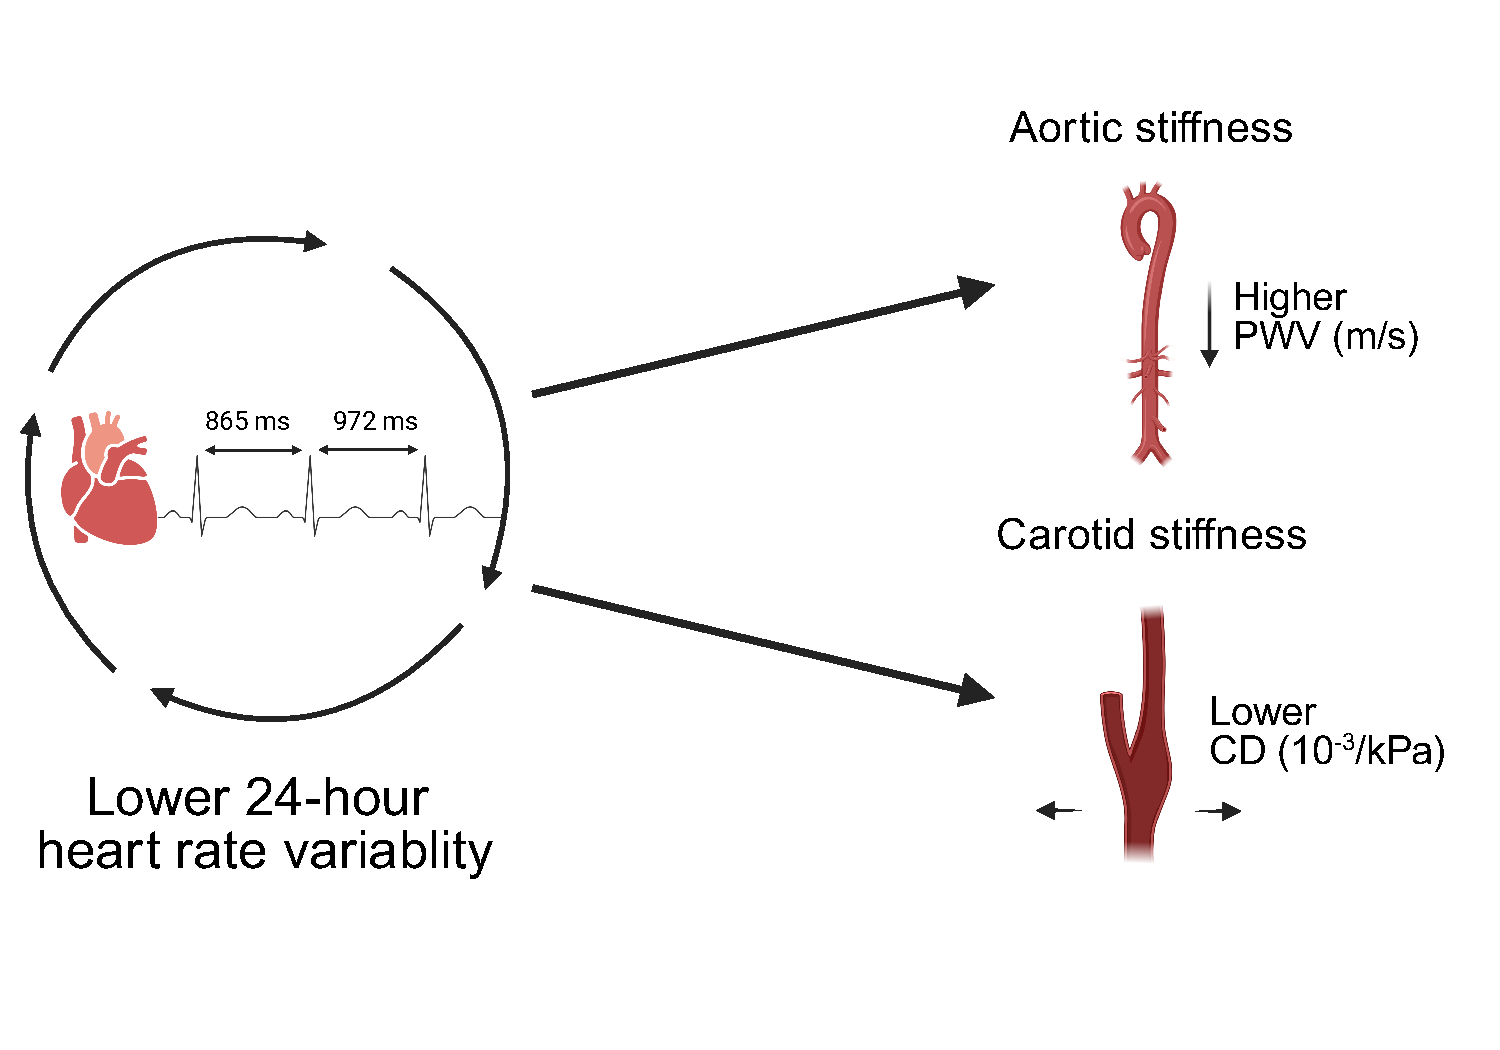
\includegraphics[width=4in,height=\textheight]{images/hrv_arterial_stiffness.pdf}

}

\caption{Autonomic dysfunction and arterial stiffness. Figure from
{[}authors{]}. ---.}

\end{figure}

Two possible mechanisms might explain how autonomic nervous function is
related to arterial stiffness. First, autonomic nervous dysfunction may
increase the vascular tone of large arteries, thereby impairing arterial
elasticity Animal studies support this notion. In rats, proper autonomic
regulation has been shown to be essential for maintaining aortic
elasticity, and heightened sympathetic activity has been shown to damage
elastin fibres, resulting in stiffer arteries. While such findings
cannot be directly extrapolated to humans, they suggest plausible
biological pathways. Second, the autonomic nervous system regulates
heart rate and cardiac contractility. Autonomic dysfunction typically
manifests as both reduced HRV and elevated resting heart rate.
{[}Arterial shear stress increases as a result of heightened sympathetic
activity and parasympathetic withdrawal.{]} A higher resting heart rate
may contribute to arterial stiffness by altering blood flow dynamics and
increasing shear stress. Our earlier study using data from the Whitehall
II cohort showed that a steeper decrease in short-term (5min) HRV over a
ten-year period was linked with higher levels of aortic stiffness in the
subsequent five years\textsuperscript{24}.

Our data from Study I, extended this perspective by showing that the
association between cardiovascular autonomic dysfunction and arterial
stiffness is modified by dysglycemia, suggesting that the autonomic
nervous system may lie on the pathway from dysglycemia to the
development of arterial stiffness, even before the onset of type 2
diabetes. Data from Whitehall II showed how aortic stiffness have a
steeper increase by higher HbA1c values among non-diabetic
individuals\textsuperscript{31}. In the subpopulation in Study I without
diabetes, we observed modification by HbA1c in both aortic and carotid
stiffness. The modifying effect of by HbA1c, suggest an amplified impact
of hyperglycemia on the consequences of autonomic dysfunction. While
several time-domain and frequency-domain HRV measures based on the
global distribution were modified by diabetes status, the association of
mean IBI was not. This suggests that the deterioration of HRV indicators
may reflect a different pathogenesis of arterial stiffness in diabetes
risk compared to heart rate.

\hypertarget{atherosclerosis-1}{%
\subsubsection{Atherosclerosis}\label{atherosclerosis-1}}

In Study II, we showed that individuals with a preclinical stage of
autonomic dysfunction, measured by week-long HRV face a higher risk of
incident ischemic-related cardiovascular disease, heart failure, and
all-cause mortality.

Multiple mechanisms may explain how autonomic dysfunction contributes to
the initiation and progression of ischemic events and stroke. First, as
discussed in Study II, autonomic dysfunction may promote
arteriosclerosis, leading to arterial stiffness. This stiffness impairs
vasodilation and may enhance vasoconstriction, increasing hemodynamic
stress and the risk of plaque rupture and thrombus
formation\textsuperscript{32}. In this context, findings from Study II
may not entirely separate between arterial stiffness and
atherosclerosis, which was been showed by data from the Rotterdam
Study\textsuperscript{33}. As plaques develop, the associated increase
in sympathetic nerve density around the arteries could reduce arterial
elasticity. In a smaller study of people with type 2 diabetes, it was
shown that lower HRV was linked with increase in carotid
atherosclerosis\textsuperscript{34}.

Second, the autonomic nervous system innervates the adventitia layer of
blood vessels, where it modulates vascular tone via sympathetic fibers.
Although atherosclerotic plaques form in the intima layer, recent in
vivo studies have demonstrated that increased plaque burden is
associated with higher local sympathetic nerve density, likely mediated
by neuroinflammatory processes. Notably, reducing sympathetic
innervation has been shown to attenuate plaque formation in animal
models\textsuperscript{35}. These findings suggest that autonomic
dysfunction may not only reflect but also actively contribute to
atherogenesis.

Third, the basis of autonomic nervous dysfunction has show to interfere
with signalling pathway controlling the heart rhythm and thus lead to
arrhythmias disturbing contraction of the heart. Data from the
Atherosclerosis Risk In Communities study of illustrated that lower
short-term HRV was associated with incident atrial fibrillation over 20
years, and the risk was higher among participants with type 2
diabetes\textsuperscript{36}. This supports autonomic dysfunctions role
in the development of arrhythmogenesis which increase the risk of MI and
stroke. However, in Study II, we do not have incident atrial
fibrillation included as an outcome, therefore it would be needed to be
explored to understand whether it could explain the higher risk of MACE.
A study of individuals with coronary artery disease showed that
stress-induced HRV was associated with myocardial infarction, even more
than resting HRV, suggesting that a lower modulation of heart rate by
parasympathetic response under stress may play a role in
ischemia\textsuperscript{37}. In our week-long recordings, our data
likely included episodes of stress-induced HRV under free-living
circumstances, e.g.~the first indication observed during the awakening
stages in the morning. Hence, capturing autonomic responses to living
circumstances and their alignment with the circadian rhythm may provide
valuable information about cardiovascular risk. Therefore, understanding
autonomic responses to tasks is relevant for comprehending their role in
cardiovascular risk, beyond short-term measures taken at rest. Including
data to monitor real-time activity, such as physical activity, would
bring additional value to capture physiological responses to bodily
demands. This could enable the inclusion of heart rate responses (e.g.,
from rest to standing) and other relevant measures of autonomic
function, such as heart rate recovery after physical movement, which is
a known risk factor for CVD and all-cause mortality
{[}\textsuperscript{\textbf{colechristopherr?}}{]}\textsuperscript{38}.

\hypertarget{heart-failure-1}{%
\subsubsection{Heart failure}\label{heart-failure-1}}

The relationship between cardiovascular autonomic dysfunction and heart
failure is complex\textsuperscript{39}. On one hand, autonomic
dysfunction may represent complication of that contributes to cardiac
stress, sympathetic overactivation, and eventual heart failure. On the
other, it may reflect the progression of cardiac remodeling and
declining cardiac output. Our findings demonstrated the relationship
between autonomic dysfunction and heart failure both cross-sectionally
in population with type 2 diabetes and prospectively in people
representing different tiers of risk of diabetes. However, our data are
limited in determining the extent to which the relationship points
toward one explanation or the other, as we lack baseline and follow-up
measures of both heart failure and HRV.

Findings from Study I confirmed the relationship between autonomic
dysfunction and arterial stiffness. It is well known that arterial
stiffness is linked to cardiac remodelling, as increased pulse wave
velocity leads to an earlier return of the reflected pulse wave to the
aorta, which increases cardiac afterload and reduces coronary perfusion
pressure\textsuperscript{40}. Therefore, arterial stiffness may have an
indirect effect on heart failure, potentially driven by autonomic
dysfunction. However, structured analyses are needed to confirm these
pathways, for example through mediation analysis to assess the direct
and indirect effects of autonomic dysfunction. In study II, we observed
that week-long HRV was linked with incident heart failure and a fourth
of the risk was explained by resting heart rate. Data from the Rotterdam
Study showed that short-term HRV was longitudinally associated with
echocardiographic measures reflecting systolic function, suggesting
autonomic dysfunction contributes to cardiac
remodelling\textsuperscript{41}. In contrast to MACE outcomes, findings
from Study II showed no specific time point in hourly HRV associated
with heart failure. Instead, it was the overall daily pattern captured
by week-long HRV that was linked to heart failure risk. This suggests
that the association is not driven by isolated shifts in autonomic
activity, but rather by a consistently impaired autonomic balance in
free-living conditions. The effect appears to be driven in part by a
failure to show appropriate decreases in heart rate during rest, as
individuals with higher hourly heart rates at night had an increased
risk of heart failure.

{[}Study III: NT-proBNP{]}

We cannot exclude the possibility that autonomic dysfunction represents
an elevated demand for compensatory mechanisms as heart failure
progresses. Studies have shown that patients with heart failure and
lower HRV tend to have a worse prognosis of mortaltity. If low HRV or
the presence of CAN were primarily driven by existing cardiac
complications, it would suggest that individuals with these conditions
exhibit more pronounced sympathetic overactivity as a consequence of
heart failure progression, and thus reverse causation. Hence, elevated
sympathetic activity during rest may indicate a greater reliance on
compensatory mechanisms to maintain cardiac output. More precise
measures are needed to assess sympathetic activity as primary driver of
heart failure or secondary compensating mechanism of cardiac
dysfunction. In addition, it remains unclear to what extent the
parasympathetic nervous system can act as a protective mechanisms to
counterbalance sympathetic dominance, and whether a decline in the
balance of HRV reflects a breakdown. The two pathways, autonomic
neuropathy and cardiac remodelling, are not mutually exclusive and may
interact in a reinforcing cycle. Autonomic dysfunction can lead to
increased sympathetic tone and reduced parasympathetic modulation,
placing the heart under chronic stress and promoting structural and
functional changes. In turn, cardiac remodeling may impair autonomic
regulation, further exacerbating the imbalance. This interplay may
create a self-perpetuating loop that accelerates the progression of
heart failure. However, this remains beyond the scope of our current
data and analysis.

\hypertarget{clinical-implications}{%
\subsection{Clinical implications}\label{clinical-implications}}

We have discussed the utility of different cohorts representing public
health, primary care, and secondary care in addressing the impact of
autonomic dysfunction on cardiovascular disease, as well as the possible
mechanisms involved. We will now focus on the clinical implications of
using autonomic dysfunction in the prevention of cardiovascular disease.
If long-term HRV or CART is to be considered for improving risk
stratification, it remains important to determine at what stage in the
progression of diabetes risk, and at which level of care, autonomic
dysfunction becomes meaningful for early detection and intervention.

\hypertarget{public-health}{%
\subsubsection{Public health}\label{public-health}}

A preventive strategy for cardiovascular disease is the identification
and treatment of high-risk individuals\textsuperscript{42}. Public
health approaches complement this by promoting healthy lifestyles,
ensuring early screening for risk factors, and improving access to
essential care and medications.

Studies I and II demonstrated a strong association between long-term HRV
and CVD risk, with particularly pronounced associations in individuals
with prediabetes and type 2 diabetes. These findings suggest that HRV
metrics could serve as early indicators for stratifying individuals who
may benefit from preventive interventions. In the Whitehall II study, we
further showed that a steeper 10-year decline in 5-minute HRV was
associated with greater aortic stiffness development over the subsequent
five years\textsuperscript{24}. Thus, a declining HRV trend detected by
smartwatches may help identify individuals who require more intensive
interventions.

Previous studies have demonstrated associations between HRV and arterial
stiffness in individuals with type 1 and type 2
diabetes\textsuperscript{43}. Building on this, our earlier work in the
Whitehall II study showed that a steeper decline in HRV was linked to
the development of arterial stiffness, even among individuals without
type 2 diabetes\textsuperscript{24}. In Study II, we extended this
perspective by examining a general population across the full spectrum
of glucose metabolism. Our findings revealed that autonomic dysfunction,
measured by long-term HRV, is consistently associated with arterial
stiffness, regardless of glycemic status. In Study I, one SD lower HRV
was equivalent to the effect of 2.7 additional years on pulse wave
velocity and 1.6 years on carotid distensibility\textsuperscript{44}. In
Study II, long-term measures of HRV were strongly associated with
cardiovascular risk, with an effect size equivalent to 4.5 additional
years of aging for major adverse cardiovascular events and 2.2 to 2.4
years for heart failure per one SD (33 ms) lower in week-long SDNN
intervals\textsuperscript{45}. Autonomic dysfunction is known to precede
the development of hypertension
{[}\textsuperscript{46}{]}\textsuperscript{47}, which is an early major
risk factor for subsequent cardiovascular disease. Our results support
the role of HRV as a early marker of cardiovascular health, in the
general population and among those with elevated cardiometabolic risk.
As such, our studies suggest that monitoring CVD risk progression or
remission through long-term HRV may be valuable.

A limitation of implementing HRV monitoring, especially for long-term
recordings, has been the demanding equipment requirements, such as the
need for ECG recorders like Holter monitors. In recent years, wearable
devices have become increasingly popular among the general
public\textsuperscript{48}. These devices offer an easy, non-invasive
way to collect heart rate and HRV data and to monitor their progression
over time. Further challenges include ensuring accurate measurement of
interbeat intervals and determining which HRV indices are most suitable
as markers of cardiovascular health. In diabetes and cardiovascular
research, 24-hour HRV measures of indices reflecting heart rate
responses to in- and expiration such as RMSSD, HF and pNN50 are more
sensitive to behavioral influences and therefore have not consistently
shown strong associations with cardiovascular or metabolic outcomes,
compared to measures based of total variability (SDNN, SDANN, TP, ULF,
VLF, LF)
{[}\textsuperscript{12}{]}\textsuperscript{16}\textsuperscript{44}.
However, the utility of these respiration-related indices appears to
improve when measured during rest in shorter segments, such as 5-minute
recordings(ref.).

If HRV monitoring proves effective by helping individuals maintain
healthy, age-adjusted HRV range through lifestyle changes, and by
prompting healthcare use in response to sustained deterioration of HRV,
then HRV could become a meaningful marker for long-term health
monitoring. A key public health challenge in integrating wearable
devices into healthcare is ensuring equitable access, as individuals
from lower socioeconomic groups are significantly less likely to own or
use such devices. This raises the risk of health disparities by
overlooking high-risk populations with lower income or education levels.
Despite these concerns, there is encouraging evidence that the general
population is open to digital health innovations. Studies have shown
that the majority of the general population is willing to share their
health data with public health institutions and to allow algorithm-based
systems, such as artificial intelligence, in collaboration with
healthcare professionals, to monitor
disease{[}\textsuperscript{48}{]}\textsuperscript{49}. Therefore,
monitoring HRV through wearable devices may serve as a first step in
tracking health status and facilitating timely referrals to primary care
when risk levels increase.

\hypertarget{primary-care}{%
\subsubsection{Primary care}\label{primary-care}}

Cardiovascular risk in primary care is assessed using clinical
evaluations and standardized risk prediction tools to identify
individuals at elevated risk (ref.). Management focuses on lifestyle
modification, pharmacological therapy, and regular monitoring to reduce
cardiovascular events (ref.). As the clinical paradigm shifts from a
focus on ischemia toward more preventive strategies targeting
atherogenesis, greater attention is being paid to individual risk
factors that predispose patients to plaque
formation\textsuperscript{50}. Individuals with prediabetes live with an
elevated cardiometabolic risk, particular ischemic CVD and heart
failure\textsuperscript{51}. This underscores the need for early and
precise risk assessment\textsuperscript{52}. Despite the increased risk,
they often remain outside structured assessment pathways in primary
care, highlighting a critical gap in preventive strategies. We will
discuss our findings to evaluate the integration of autonomic function
assessment into routine cardiovascular risk stratification, with a
particular emphasis on individuals with prediabetes or type 2 diabetes.

A central question that arises is whether autonomic dysfunction can
serve not only as a potential marker of underlying pathophysiology but
also as a clinically useful risk indicator for CVD and heart failure. If
so, it could help identify patients at higher risk and thereby improve
risk stratification. This concept can be explored from two complementary
perspectives. First, long-term measurements of HRV may enhance the
precision of individual cardiovascular risk prediction when added to
established clinical risk scores. Second, these measurements may help
identify preclinical manifestations of cardiovascular autonomic
dysfunction, enabling targeted interventions in a subgroup of patients
to prevent future CVD.

This raises the question of whether incorporating long-term HRV into
traditional cardiovascular risk models, such as the Systematic COronary
Risk Evaluation 2 (SCORE-2) and the Framingham Risk Score, adds
meaningful predictive value\textsuperscript{53,54}.Our findings in Study
I support a potential added value of 24-hour HRV to arterial stiffness,
which is considered a surrogate marker of cardiovascular disease risk.
In Study II, we extended this perspective by demonstrating a link
between multiday HRV and hard endpoints of CVD and heart failure.
However, our findings are based on associations and do not include
prediction of outcomes\textsuperscript{55}. Therfore, a limitation of
our study is that we did not evaluate whether incorporating long-term
HRV or CARTs into established risk scores improves detection compared to
existing guidelines for cardiovascular disease and heart failure. While
most biomarkers have shown limited incremental value beyond established
predictors such as age, sex, lipid levels, diabetes status, and blood
pressure, some studies suggest that 24-hour HRV may improve risk
discrimination for cardiovascular disease and all-cause mortality in
individuals with type 2 diabetes\textsuperscript{56}, and for stroke in
older adults\textsuperscript{57}. However, a key limitation of these
studies is that their reference models have not been calibrated or
validated on a large scale cohorts, and in combination with established
risk scores such as SCORE2 and the Framingham Risk Score.

Increasing availability of wearable devices capable of capturing
long-term HRV data presents a practical opportunity for continuous
monitoring in primary care settings. Wearable devices may facilitate
earlier detection of autonomic dysfunction and support more personalized
approaches to prevention and management of CVD risk. However, the
clinical utility of stratifying patients based on preclinical autonomic
dysfunction remains uncertain. These considerations are only actionable
if interventions targeting autonomic function can be shown to reduce
cardiovascular risk. Emerging evidence suggests that both
pharmacological and lifestyle interventions can improve HRV in the short
term\textsuperscript{27,58}. For example, high-intensity interval
training has been shown to improve autonomic function in obese
individuals with and without type 2 diabetes, although benefits in HRV
were observed only in those without diabetes\textsuperscript{59}.
Similarly, lifestyle changes in individuals with prediabetes have been
associated with improvements in short-term HRV, which may partly explain
the reduction in diabetes risk independently of weight
loss\textsuperscript{60}.

Nevertheless, it remains unclear whether these effects are sustainable
over time and whether they translate into long-term cardiovascular
protection. Particularly in the context of lifestyle improvements and
intensified diabetes management, much of the observed enhancement in
autonomic function may be mediated indirectly through improvements in
cardiometabolic markers such as glucose levels, lipid profiles, body
weight, maximal oxygen uptake, and blood pressure. Despite current
uncertainties, monitoring autonomic function through long-term HRV may
offer a valuable tool for assessing cardiovascular risk and tracking the
impact of preventive strategies. However, its clinical utility must be
confirmed through robust evidence demonstrating sustained effects and
improved cardiovascular outcomes.

\hypertarget{secondary-care}{%
\subsubsection{Secondary care}\label{secondary-care}}

In secondary care, endocrinologists assess cardiovascular and heart
failure risk management by integrating advanced diagnostics, biomarker
analysis, and imaging to detect early dysfunction. Treatment of patients
with type 2 diabetes is guided by evidence-based therapies and
multidisciplinary collaboration. The ADA/EASD 2022 consensus of
\emph{Management of Hyperglycemia in Type 2 Diabetes} emphasizes that
early detection of HF in individuals with T2D is crucial, as it enables
timely initiation of therapies such as SGLT2i, which have demonstrated
significant benefits in reducing HF-related
outcomes\textsuperscript{61}. A major challenge in diabetes care is
detecting heart failure before symptoms appear, as patients with
symptomatic heart failure face a higher risk of mortality and more
frequent hospitalizations\textsuperscript{62}. The AHA, ACC, and HFSA
2022 guideline recommends identifying individuals at risk of heart
failure based on factors such as diabetes, poor glycaemic control,
uncontrolled hypertension, hyperlipidaemia, elevated body mass index,
albuminuria, renal dysfunction, and a history of
CVD\textsuperscript{63}. Still, there is a need to identify the optimal
approach to recognize and diagnose heart failure in clinical care, as
broad screening of echocardiography in type 2 diabetes is time-consuming
and costly to perform\textsuperscript{62}.

We demonstrated that CAN may help identify individuals at increased risk
of heart failure, beyond what is captured by symptoms or existing risk
scores. Therefore, our findings support considering CAN as a relevant
risk factor for heart failure and suggest it may have value in future
risk stratification strategies in type 2 diabetes. The clinical
advantage on using CARTs is a standardized test under specific
conditions. As we discusses, the tests is reliable and reproducible,
with reference values in a large population\textsuperscript{29}. Beyond
our findings and the established evidence of increased heart failure
risk, CAN in the type 2 diabetes population also identifies individuals
at high risk for cardiovascular disease, kidney disease, and early
mortality. In Study III, we observed that two out of five participants
had CAN, highlighting it as a prevalent complication. Therefore,
detecting CAN may uncover an often-overlooked condition that is common
in individuals with type 2 diabetes.

The clinical stratification of care includes two key considerations: (1)
CAN should be further evaluated for associated cardiovascular
complications, such as heart failure; and (2) cardiopreventive
strategies should be initiated earlier in this subgroup.

First, patients with CAN may benefit from further cardiovascular
assessment, such as the use of sensitive biomarkers or echocardiography.
NT-proBNP is a strong predictor of heart failure and a validated
biomarker for ruling out the condition (ref.). However, its specificity
varies across heart failure phenotypes, being less specific for
detecting HFpEF compared to HFrEF. Therefore, additional evaluation
using echocardiography is warranted. Echocardiography not only helps
classify heart failure phenotypes but also identifies preclinical stages
of heart failure through the detection of functional or structural
cardiac abnormalities. An important question remains: to what extent
does CAN overlap with cardiac abnormalities identified via
echocardiography? Including CAN in structured assessments of heart
failure could help clarify this relationship. Determining the diagnostic
and prognostic value of CAN, particularly its sensitivity and
specificity in detecting HFrEF and HFpEF, requires further
investigation.

Second, the presence of CAN may justify the earlier initiation of
protective therapies. SGLT2 inhibitors are recommended as second-line
treatment in type 2 diabetes and have demonstrated benefits in reducing
the risk of heart failure, cardiovascular disease, and kidney function
decline, complications commonly associated with CAN. Current guidelines
recommend initiating these therapies based on a history of
cardiovascular disease, heart failure or the presence of conventional
high-risk CVD factors. However, the specific impact of SGLT2 inhibitors
on the progression of cardiorenal outcomes in patients with CAN remains
to be fully understood. Furthermore, while anti-hypertensive treatment
is a cornerstone of cardiovascular risk management, whether specific
classes of anti-hypertensive agents offer protective effects in patients
with CAN remains to be explored.

The extent of our findings is limited in terms of clinical implications
in Study III. First, the generalizability of our results is restricted,
as our study population consists of patients with type 2 diabetes
receiving secondary care. We observed that two out of five patients with
CAN also had a history of cardiovascular disease, a group already at
increased risk due to their diagnosis. This overlap may influence the
interpretation of CAN as an independent risk factor. Therefore, our
findings need to be validated in a broader population with type 2
diabetes, including individuals without a history of CVD. Doing so would
allow for greater generalizability of our results to the broader type 2
diabetes population, particularly patients in primary care.

\bookmarksetup{startatroot}

\hypertarget{perspective-will-be-rewritten}{%
\chapter{Perspective {[}will be
rewritten{]}}\label{perspective-will-be-rewritten}}

We have discussed the mechanisms and clinical implications of
cardiovascular autonomic function across different stages of glucose
metabolism. Based on our findings and discussion, we propose further
perspectives to define its role in research and healthcare from three
aspects: (1) continuous non-invasive health monitoring, (2) risk
stratification, and (3) identification as a causal and modifiable
marker.

\hypertarget{continuous-monitoring-of-cardiovascular-health}{%
\section{Continuous monitoring of cardiovascular
health}\label{continuous-monitoring-of-cardiovascular-health}}

Wearable devices enables comprehensive data collection on behavioral
(e.g., sleep and physical activity) and physiological (e.g., heart rate,
ECG, temperature) parameters\textsuperscript{64}. These devices offer a
broader and more feasible approach to long-term heart rate monitoring.
Despite growing interest in wearable-based monitoring, the integration
of HRV into routine cardiometabolic risk assessment remains limited.

Two key aspects highlight the potential applications of monitoring: (1)
identification of risk and (2) assessment of response to intervention.

\emph{Identification of risk}

Understanding when and how physiological signals reflect elevated CVD
risk is essential for developing early and effective prevention
strategies. In Study II, we observed that specific morning time points
were associated with increased CVD risk, indicating that physiological
responses captured under free-living conditions may provide meaningful
insights into early risk detection. Rather than adjusting for physical
activity as a confounding factor, future predictive models could benefit
from integrating multiple physiological signals, including HRV, sleep,
and activity patterns, to better reflect dynamic states of health.
Machine learning techniques offer the ability to process complex raw
time-series data, such as interbeat intervals and accelerometer signals,
and to uncover patterns that may improve risk prediction beyond
conventional summary measures of HRV. However, a key limitation of these
models is their reduced explainability, which may limit their clinical
applicability. Incorporating HRV into digital health platforms could
support personalized feedback mechanisms, enabling timely lifestyle or
therapeutic interventions and contributing to more adaptive and
preventive healthcare strategies.

\emph{Assessment of response to intervention}

HRV highlights a potential target for intervention, given that low HRV
may be indicative of adverse lifestyle patterns. For instance,
behavioral patterns such as disrupted sleep or irregular meal timing may
influence circadian fluctuations in HRV. Evidence from studies on
night-shift workers suggests that meal timing affects HRV, with daytime
meals leading to higher HRV during night hours\textsuperscript{27}.
Medications such as beta-blockers and GLP-1 receptor agonists have been
shown to influence autonomic function, with effects observed in both
24-hour and hourly HRV
measures{[}\textsuperscript{25}{]}\textsuperscript{65}.

\begin{figure}

\begin{minipage}[t]{\linewidth}

{\centering 

\raisebox{-\height}{

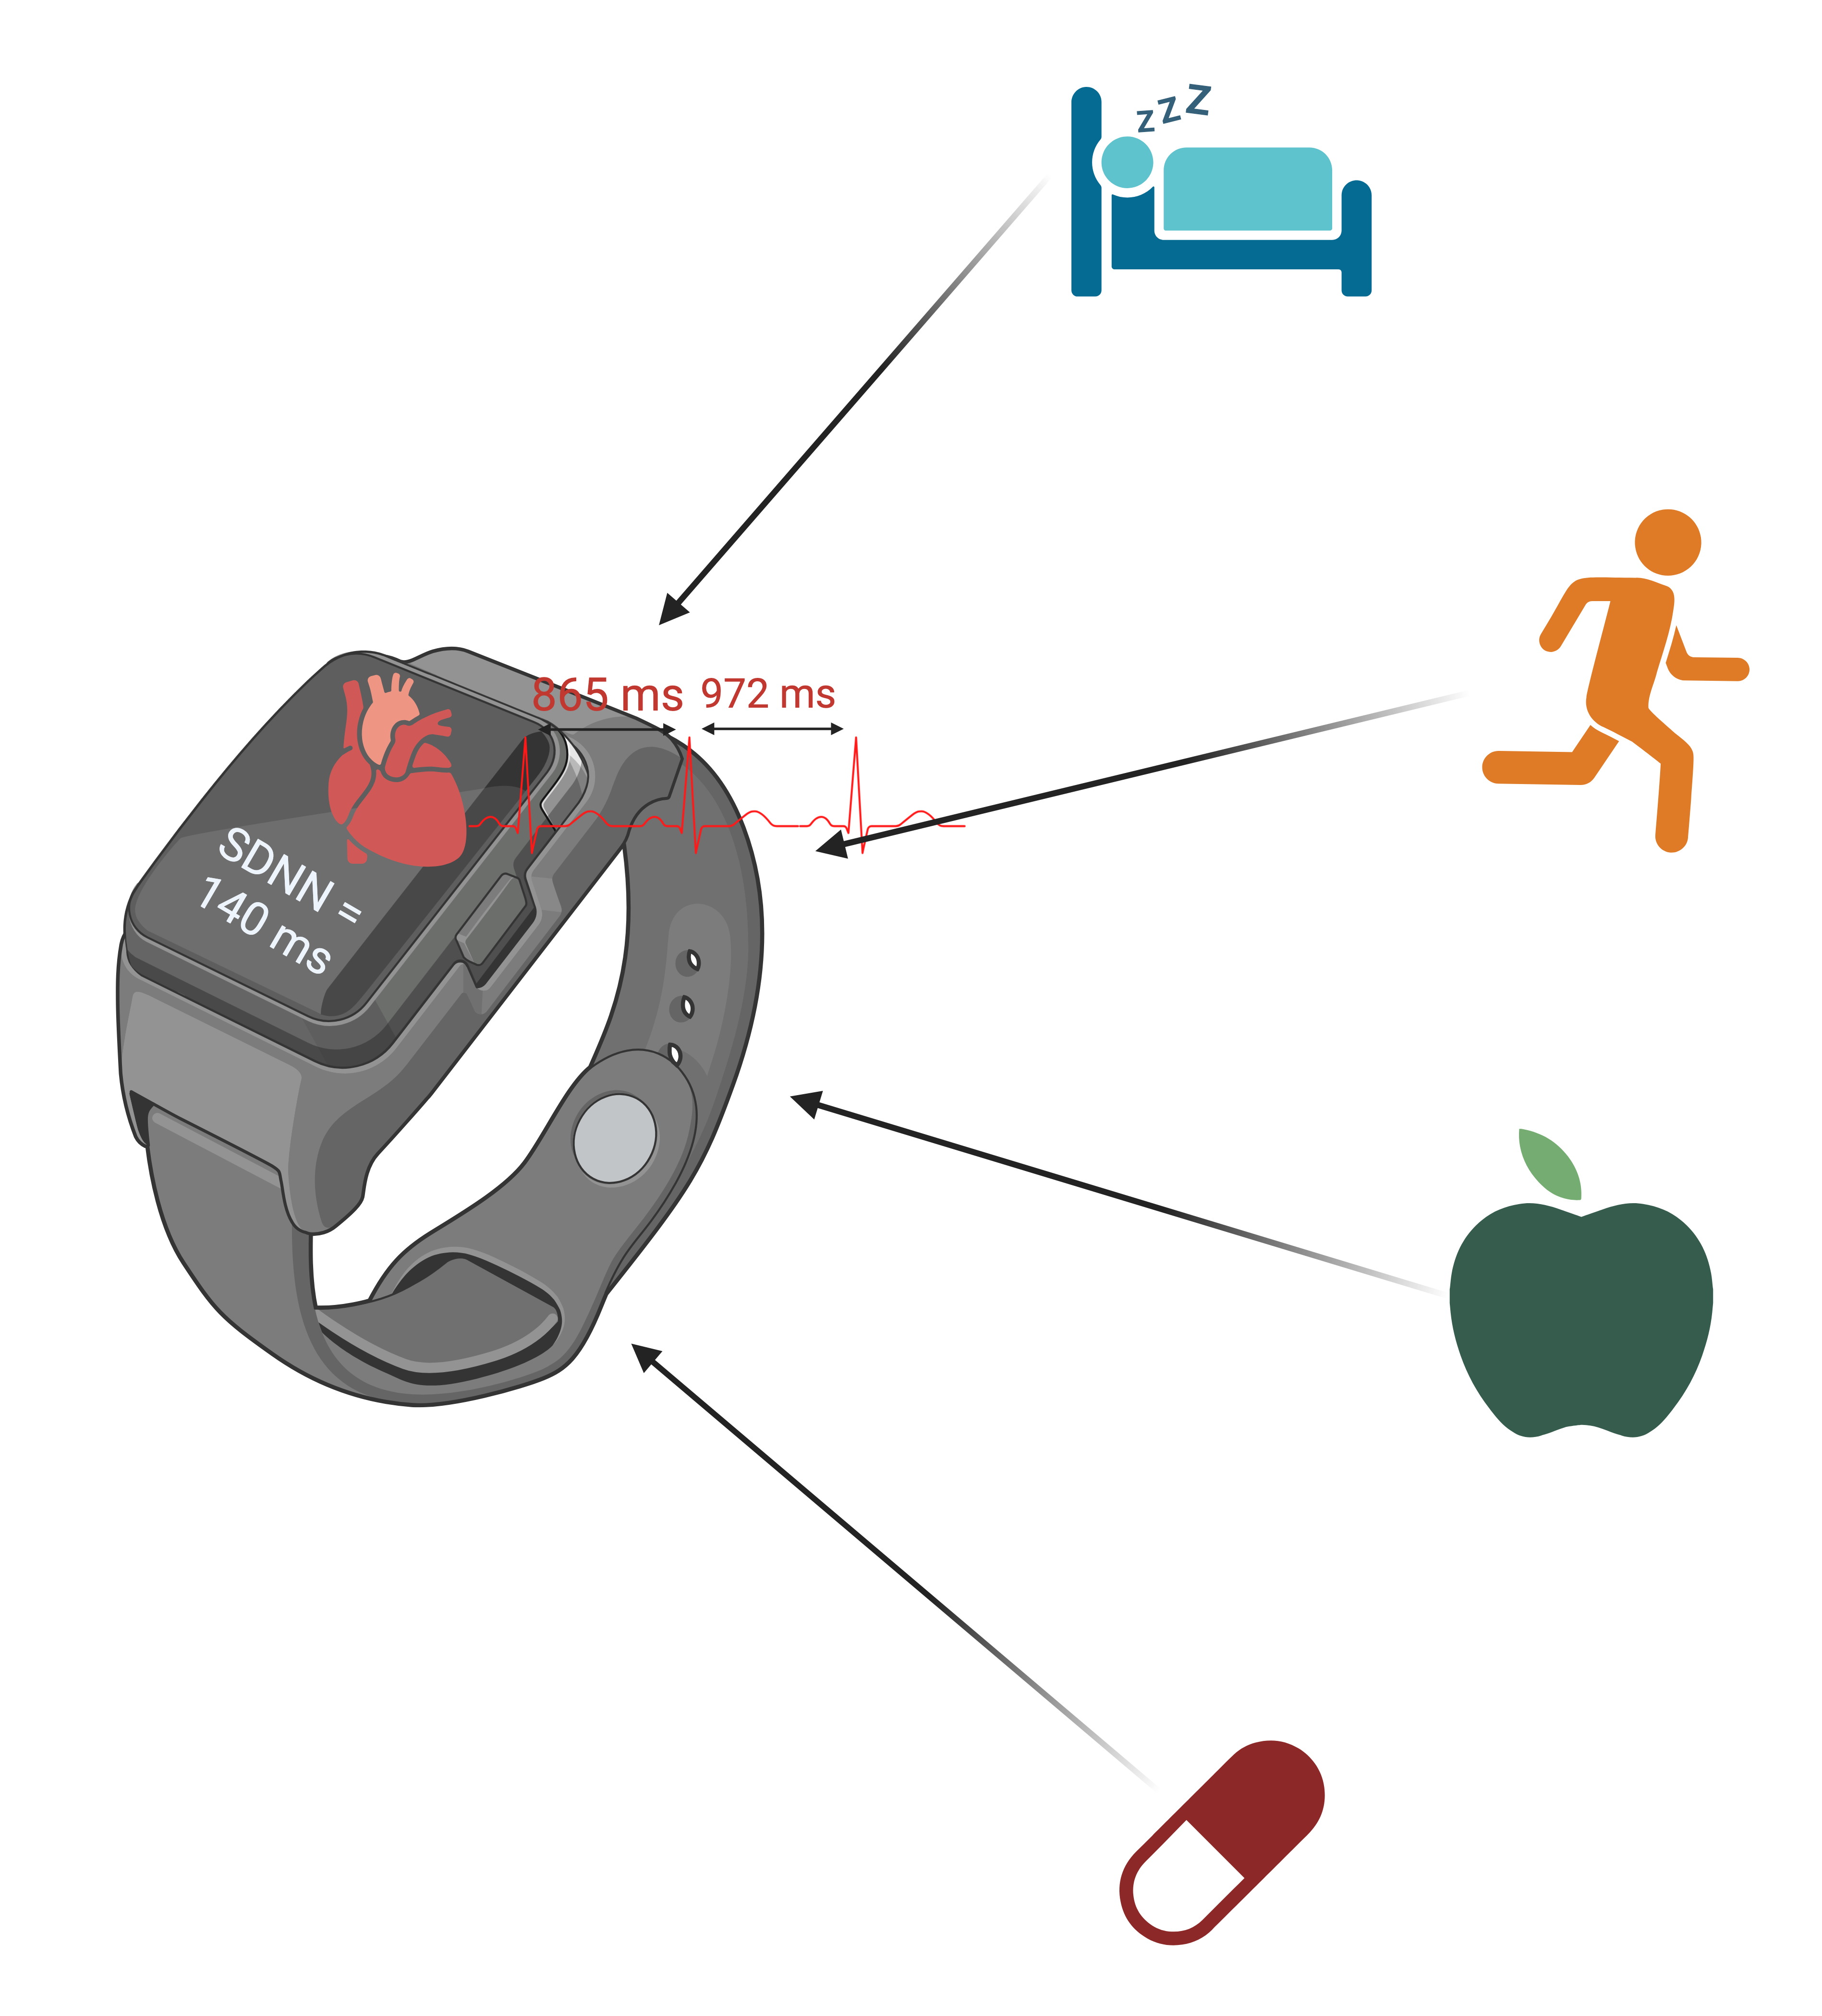
\includegraphics[width=4in,height=\textheight]{images/smartwatch.png}

}

\caption{Biofeedback HRV response to lifestyle and treatment solutions}

}

\end{minipage}%

\end{figure}

Hence, future studies can leverage wearable devices to continuously
monitor risk by HRV and better understand the behavioral factors and
treatment options that contribute to its improvement or deterioration.
This approach may help identify effective lifestyle patterns or
medications that improve cardiovascular health through modulation of
HRV. Hourly measures serves

However, standardization and transparency across different brands of
wearable devices remain a challenge for both research and clinical
implementation of heart rate and HRV monitoring. While smartwatches
offer a convenient method for heart rate measurement, their accuracy can
vary, as they rely on photoplethysmography to detect pulse rate at the
wrist. This method can be imprecise under certain conditions,
particularly during physical activity, due to motion artifacts and other
external factors\textsuperscript{66}. Despite these limitations, ongoing
improvements in sensor technology and algorithm calibration are likely
to enhance the reliability of wearable-derived heart rate and HRV data.

\hypertarget{risk-stratification-1}{%
\section{Risk-stratification}\label{risk-stratification-1}}

Individuals with elevated glucose levels in prediabetic stage are at
increased risk of developing metabolic complications and CVD. However,
many remain metabolically stable or even return to normal glucose
regulation over time. As a result, structured treatment strategies for
this group have not been widely adopted in clinical practice. This is
partly due to the high degree of heterogeneity within this population.
Therefore, additional indicators beyond glucose levels may be useful to
identify those most likely to benefit from early intervention.

Our findings suggest that HRV may serve as a valuable marker among
individuals at elevated cardiovascular risk, helping to identify those
who could benefit from targeted preventive strategies. Future research
should evaluate whether individuals classified as high-risk based on
autonomic dysfunction respond to specific interventions

In the context of wearable devices, it remains to be determined whether
HRV can serve as an early indicator of CVD risk alongside simple markers
such as age, sex, and BMI, and whether it may enable risk identification
before more invasive measures, such as blood-based biomarkers, are
considered.

A limitation of long-term HRV measurement is the lack of
standardization, as data are collected under free-living conditions and
may be influenced by daily behaviors, potentially affecting risk
classification. Hence, standardized procedures may be needed. CART has
been shown to be reliable non-invasive and typically takes approximately
10 minutes to complete.

In Study III, we demonstrated a relationship between CAN and cardiac
dysfunction, as measured by NT-proBNP. Heart failure is characterized by
both structural and functional changes in the heart, such as left
ventricular dysfunction, which can be assessed using echocardiography.
However, the link between these structural and functional changes and
their impact on systolic and diastolic pumping function in relation to
CAN remains to be fully understood. Furthermore, the diagnostic and
prognostic value of CAN, particularly its sensitivity and specificity in
detecting HFrEF and HFpEF, requires further investigation.

::: \{layout-ncol=``1''\}
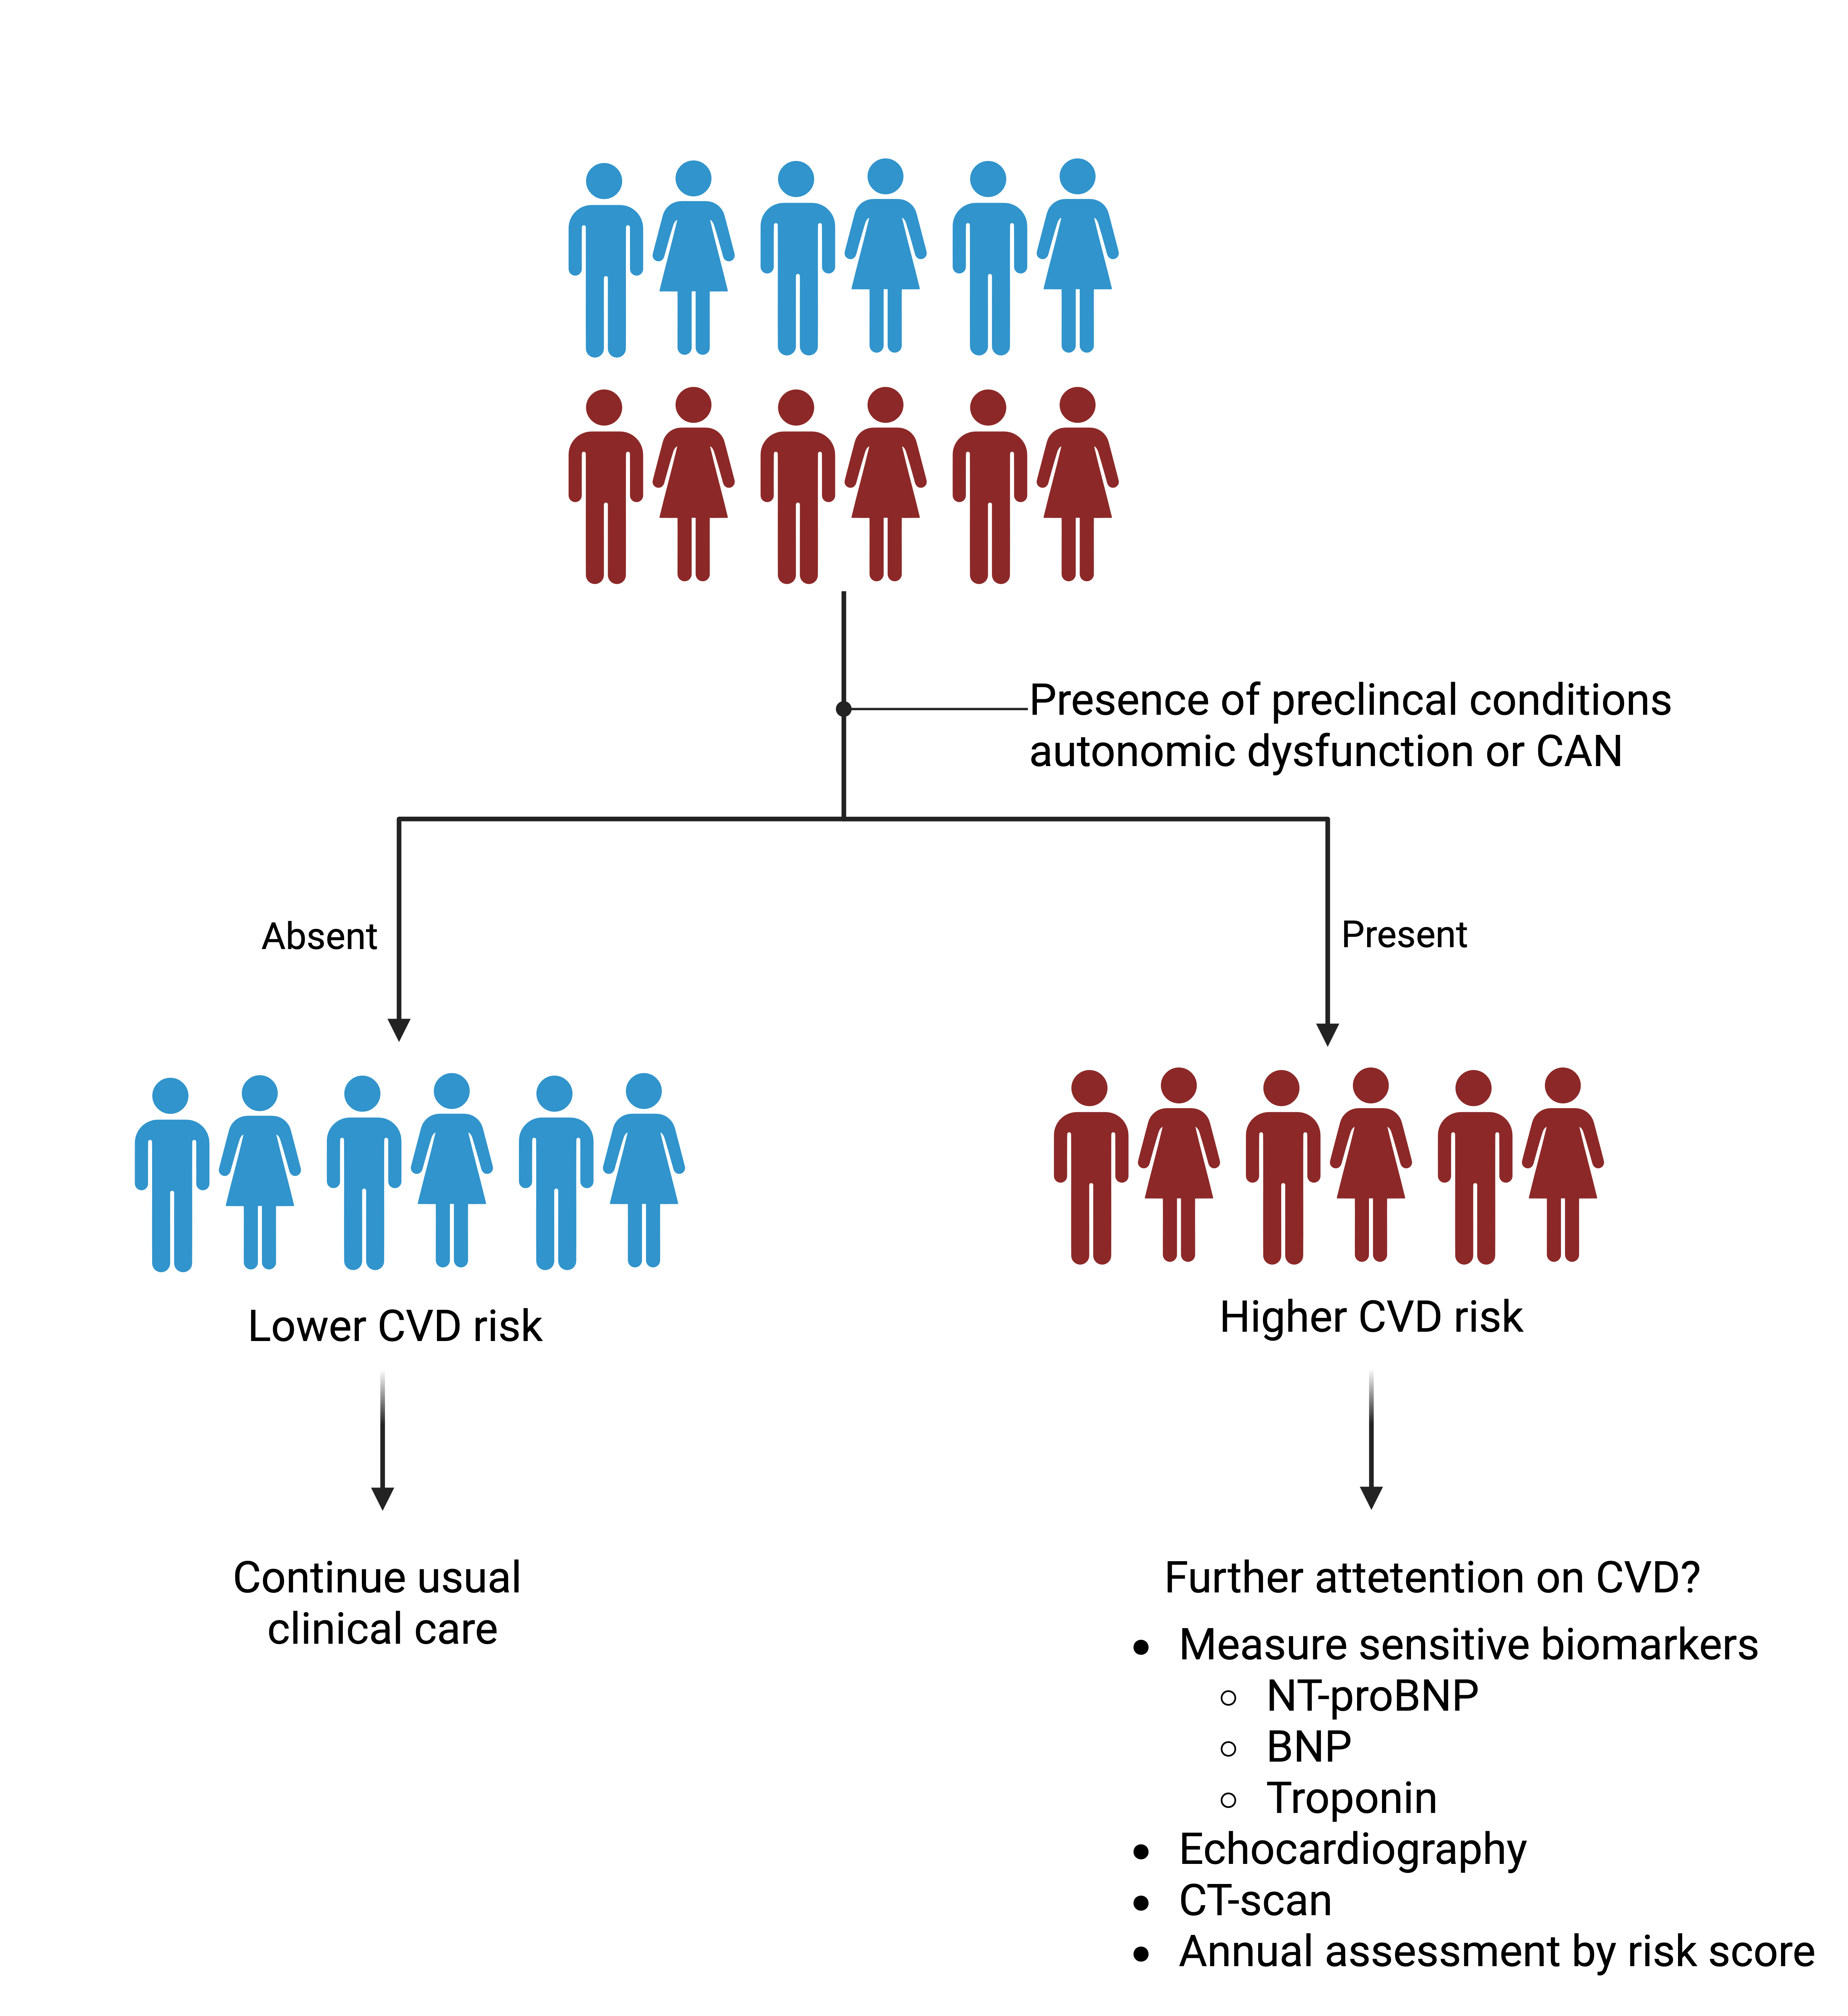
\includegraphics[width=5in,height=\textheight]{images/strafication_tree_of_CAN.png}
:::

\hypertarget{effective-causal-modifiable-marker}{%
\section{Effective causal modifiable
marker}\label{effective-causal-modifiable-marker}}

\begin{itemize}
\tightlist
\item
  clinical trails
\item
  lifestyle intervention
\end{itemize}

Our findings in Studies I and II support the etiological link between
long-term HRV and the risk of CVD, which provide a first line of
evidence of a causal relationship. However, the observed association
does not imply causation, and further research is necessary to determine
whether the relationship between HRV and CVD risk is indeed causal.
Traditionally, epidemiological research has relied on randomized
controlled trials to establish causal relationships. However, conducting
such trials to isolate the direct of HRV is particularly challenging.
Interventions that modify HRV often do so indirectly, through changes in
lifestyle factors such as weight loss, inflammation, or insulin
sensitivity, or through pharmacological treatments like blood pressure
medications. As a result, isolating the direct modification of HRV is
difficult. To address these limitations, modern epidemiological
approaches such as Mendelian randomization (MR)\textsuperscript{67} and
structured causal mediation analysis offer promising alternatives for
inferring causality from observational data {[}modern epidemiology 4th
edition{]}.

A genome-wide association study (GWAS) has identified 17 lead single
nucleotide polymorphisms (SNPs) across eight loci associated with HRV
based on short-term recordings, suggesting the potential for these
variants to serve as genetic instruments in Mendelian randomization
analyses\textsuperscript{68}. Another study demonstrated that
phenotypically measured HRV was associated with all-cause mortality but
found no evidence of a genetic association between genes linked to HRV
and all-cause mortality\textsuperscript{69}. To date, no GWAS has been
conducted to investigate the genetic determinants of long-term HRV.
Establishing such genetic associations is essential for understanding
its genetic architecture and for providing unconfounded estimates by
using genetic variants as proxies to assess the causal role of HRV in
CVD.

\begin{figure}

\begin{minipage}[t]{\linewidth}

{\centering 

\raisebox{-\height}{

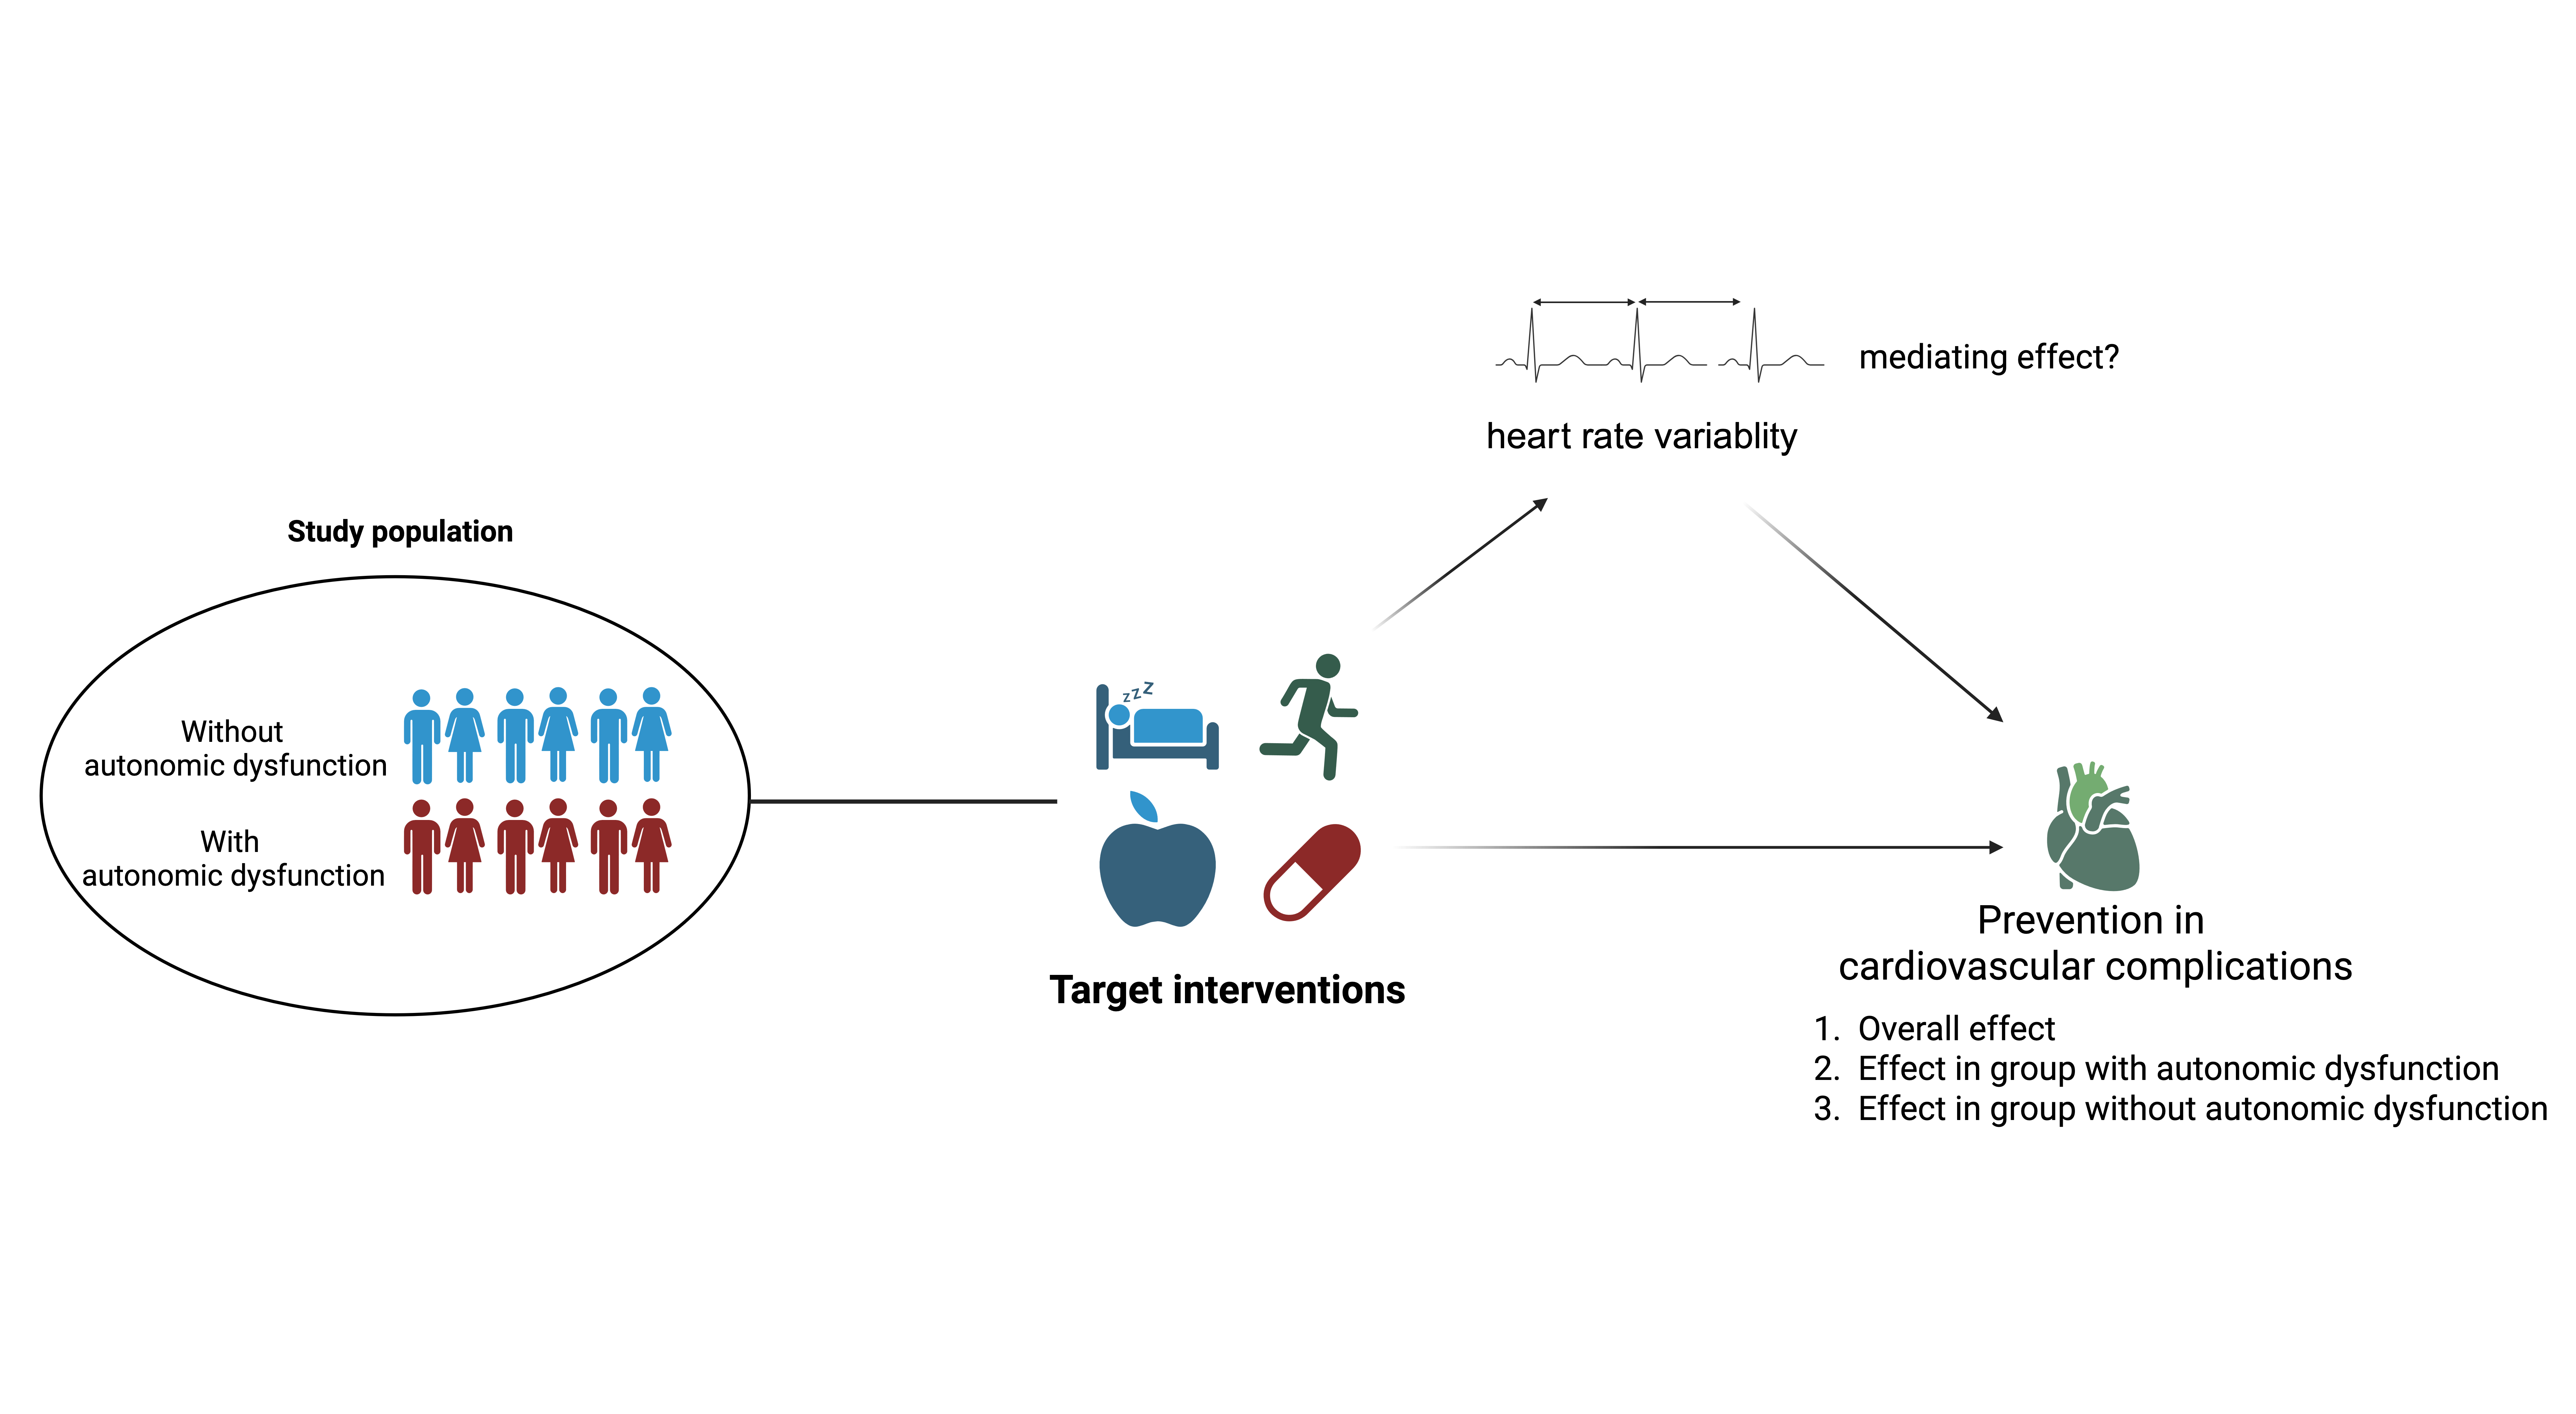
\includegraphics[width=6in,height=\textheight]{images/Mediation_HRV.png}

}

\caption{Mediation of HRV by intervention in prevention of CVD}

}

\end{minipage}%

\end{figure}

A study have demonstrated that reduced HRV mediates the association
between glomerular hyperfiltration and mortality\textsuperscript{70},
indicating an initial potential for HRV as a modifying factor. While
this has been shown in observational data, no evidence of such mediation
has yet been established in trial data. The Diabetes Prevention Program
(DPP) showed that HRV may modify the effect of lifestyle intervention in
preventing type 2 diabetes\textsuperscript{60}. However, it remains
unclear to what extent this modification applies to cardiovascular
outcomes, and whether the intervention was more effective among
individuals with lower HRV. Cardiometabolic intervention trials, whether
focused on lifestyle modification or pharmacological treatment, should,
where feasible, include HRV measurements to enable structured mediation
analyses and to better understand the role of autonomic function in
cardiovascular outcomes. This could help demonstrate whether
modification of HRV through potential strategies such as medications
like beta-blockers or lifestyle interventions including physical
activity, diet, and sleep has a sustainable effect on CVD outcomes.

Earlier studies have shown an association between autonomic dysfunction,
as measured by short-term HRV during rest, and arterial
stiffness\textsuperscript{43}{[}add cvd{]}. In Study I, we extended
perspective of but long-term HRV, does link with arterial stiffness,
suggesting autonomic response to free-living conditions contribute to
the development of arterial stiffness. In addition, we found that HRV
was associated with locally measured carotid distensibility. However,
our results are limited by the inability to distinguish between
sympathetic and parasympathetic contributions to arterial stiffness, or
to determine whether the observed risk is driven by specific responses
to living conditions or circadian rhythm variations.

As increased sympathetic nervous system activity has been linked to
greater plaque formation, and may be modifiable by reducing sympathetic
drive, the autonomic nervous system could play a role in reducing
atherosclerotic thrombus formation. However, more physiological studies
are needed to understand the mechanisms of atherosclerosis in the
presence of autonomic nervous dysfunction, including the causal
direction between the two, and how this interplay may be altered during
the progression from normal glucose metabolism to type 2 diabetes. This
requires more precise measures of both sympathetic and parasympathetic
activity, as well as markers of endothelial dysfunction, beyond what is
currently captured by HRV and common indices of arterial stiffness.

{[}Thus, although long-term HRV may lack the precision to disentangle
sympathetic and parasympathetic activity due to overlapping behavioral
and physiological influences, it may be a valuable tool for assessing
autonomic responses in free-living conditions and informing
lifestyle-based strategies to improve cardiovascular health. Hence, HRV
show potential as a responsive marker to monitor successfullness in CVD
risk management.{]}

\bookmarksetup{startatroot}

\hypertarget{conclusion-will-be-rewritten}{%
\chapter{Conclusion {[}will be
rewritten{]}}\label{conclusion-will-be-rewritten}}

Autonomic dysfunction, assessed through 24-hour HRV, is associated with
increased arterial stiffness. This relationship is already evident in
individuals with normal glucose metabolism and becomes more pronounced
in those with prediabetes and type 2 diabetes. In individuals at high
risk of type 2 diabetes, lower long-term HRV measured over a week has
been linked to ischemic events, heart failure, and all-cause mortality,
highlighting HRV's potential as a marker of cardiovascular health. Both
HRV and heart rate follow circadian patterns in relation to
cardiovascular events. Higher nighttime heart rate is associated with
increased risk of heart failure, and specific morning patterns of HRV
have been linked to ischemic events. These findings suggest that both
long-term and hourly HRV measures provide valuable prognostic
information. Structured testing of cardiovascular autonomic function in
individuals with type 2 diabetes can detect those with CAN and may help
identify individuals at higher risk of heart failure.

We have established an association between HRV and cardiovascular
complications. However, the underlying mechanism remains unclear. It is
not yet known whether autonomic dysfunction, as indicated by low HRV, is
a marker of developing arteriosclerosis, atheroma, or cardiac
remodeling, or whether it plays a causal role in their development.
While the pathogenic pathways leading to cardiovascular risk appear
similar across the spectrum of glucose metabolism, dysglycemia may
amplify the impact of autonomic dysfunction. Whether lower long-term HRV
in individuals with prediabetes or type 2 diabetes reflects a distinct
physiological mechanism involving neuropathy, compared to those with
normal glucose metabolism, remains an open question. When using HRV and
standardized CART, it is important to carefully consider how the data
are applied in relation to the specific research objectives, ranging
from physiological mechanisms to clinical diagnosis.

Structured studies assessing screening strategies and trial designs,
whether focused on lifestyle interventions or targeted pharmacological
modulation of HRV, are needed to clarify the clinical role of HRV and
CART in cardiovascular prevention. Long-term HRV and its hourly
fluctuations provide insight into autonomic responses under free-living
conditions. Further research is needed to determine whether modifying
these measures can yield sustained preventive effects on cardiovascular
disease and mortality. CARTs offer a standardized approach for
diagnosing CAN. Clarifying the clinical utility of CARTs in assessing
cardiovascular and heart failure risk through the identification of CAN
is essential for advancing precision care in individuals with type 2
diabetes. Echocardiographic studies can help establish the link between
CAN and the risk of specific heart failure subtypes. Future research
should carefully select HRV measures aligned with specific clinical or
research objectives. Long-term HRV and CART have demonstrated potential
in cardiovascular risk assessment and should be integrated to evaluate
whether autonomic function assessments can monitor treatment or
lifestyle effectiveness, or guide stratified cardiovascular risk
decisions in individuals with prediabetes or type 2 diabetes.

\bookmarksetup{startatroot}

\hypertarget{references}{%
\chapter*{References}\label{references}}
\addcontentsline{toc}{chapter}{References}

\markboth{References}{References}

\hypertarget{refs}{}
\begin{CSLReferences}{0}{0}
\leavevmode\vadjust pre{\hypertarget{ref-yusuf2020}{}}%
\CSLLeftMargin{1 }%
\CSLRightInline{Yusuf S, Joseph P, Rangarajan S, \emph{et al.}
\href{https://doi.org/10.1016/S0140-6736(19)32008-2}{Modifiable risk
factors, cardiovascular disease, and mortality in 155{\hphantom{,}}722
individuals from 21 high-income, middle-income, and low-income countries
(PURE): A prospective cohort study}. \emph{The Lancet} 2020;
\textbf{395}: 795--808.}

\leavevmode\vadjust pre{\hypertarget{ref-lu2023}{}}%
\CSLLeftMargin{2 }%
\CSLRightInline{Lu Y, Kiechl SJ, Wang J, Xu Q, Kiechl S, Pechlaner R.
\href{https://doi.org/10.1016/j.ebiom.2023.104619}{Global distributions
of age- and sex-related arterial stiffness: systematic review and
meta-analysis of 167 studies with 509,743 participants}.
\emph{EBioMedicine} 2023; \textbf{92}: 104619.}

\leavevmode\vadjust pre{\hypertarget{ref-shah2015}{}}%
\CSLLeftMargin{3 }%
\CSLRightInline{Shah AD, Langenberg C, Rapsomaniki E, \emph{et al.}
\href{https://doi.org/10.1016/S2213-8587(14)70219-0}{Type 2 diabetes and
incidence of cardiovascular diseases: A cohort study in 1·9 million
people}. \emph{The Lancet Diabetes \& Endocrinology} 2015; \textbf{3}:
105--13.}

\leavevmode\vadjust pre{\hypertarget{ref-donnan2008}{}}%
\CSLLeftMargin{4 }%
\CSLRightInline{Donnan GA, Fisher M, Macleod M, Davis SM.
\href{https://doi.org/10.1016/S0140-6736(08)60694-7}{Stroke}. \emph{The
Lancet} 2008; \textbf{371}: 1612--23.}

\leavevmode\vadjust pre{\hypertarget{ref-vos2020}{}}%
\CSLLeftMargin{5 }%
\CSLRightInline{Vos T, Lim SS, Abbafati C, \emph{et al.}
\href{https://doi.org/10.1016/S0140-6736(20)30925-9}{Global burden of
369 diseases and injuries in 204 countries and territories,
1990{\textendash}2019: A systematic analysis for the global burden of
disease study 2019}. \emph{The Lancet} 2020; \textbf{396}: 1204--22.}

\leavevmode\vadjust pre{\hypertarget{ref-li2024}{}}%
\CSLLeftMargin{6 }%
\CSLRightInline{Li X, Kong X, Yang C, \emph{et al.} Global, regional,
and national burden of ischemic stroke, 1990{\textendash}2021: An
analysis of data from the global burden of disease study 2021.
\emph{eClinicalMedicine} 2024; \textbf{75}.
DOI:\href{https://doi.org/10.1016/j.eclinm.2024.102758}{10.1016/j.eclinm.2024.102758}.}

\leavevmode\vadjust pre{\hypertarget{ref-lee2012}{}}%
\CSLLeftMargin{7 }%
\CSLRightInline{Lee M, Saver JL, Hong K-S, Song S, Chang K-H, Ovbiagele
B. \href{https://doi.org/10.1136/bmj.e3564}{Effect of pre-diabetes on
future risk of stroke: Meta-analysis}. \emph{BMJ : British Medical
Journal} 2012; \textbf{344}: e3564.}

\leavevmode\vadjust pre{\hypertarget{ref-barr2007}{}}%
\CSLLeftMargin{8 }%
\CSLRightInline{Barr ELM, Zimmet PZ, Welborn TA, \emph{et al.}
\href{https://doi.org/10.1161/CIRCULATIONAHA.106.685628}{Risk of
cardiovascular and all-cause mortality in individuals with diabetes
mellitus, impaired fasting glucose, and impaired glucose tolerance}.
\emph{Circulation} 2007; \textbf{116}: 151--7.}

\leavevmode\vadjust pre{\hypertarget{ref-normand2019}{}}%
\CSLLeftMargin{9 }%
\CSLRightInline{Normand C, Kaye DM, Povsic TJ, Dickstein K.
\href{https://doi.org/10.1016/S0140-6736(18)32216-5}{Beyond
pharmacological treatment: An insight into therapies that target
specific aspects of heart failure pathophysiology}. \emph{The Lancet}
2019; \textbf{393}: 1045--55.}

\leavevmode\vadjust pre{\hypertarget{ref-campbell2024}{}}%
\CSLLeftMargin{10 }%
\CSLRightInline{Campbell P, Rutten FH, Lee MM, Hawkins NM, Petrie MC.
\href{https://doi.org/10.1016/S0140-6736(23)02756-3}{Heart failure with
preserved ejection fraction: everything the clinician needs to know.}
\emph{Lancet (London, England)} 2024; \textbf{403}: 1083--92.}

\leavevmode\vadjust pre{\hypertarget{ref-schlaich2015}{}}%
\CSLLeftMargin{11 }%
\CSLRightInline{Schlaich M, Straznicky N, Lambert E, Lambert G.
\href{https://doi.org/10.1016/s2213-8587(14)70033-6}{Metabolic syndrome:
a sympathetic disease?} \emph{Lancet Diabetes Endocrinol} 2015;
\textbf{3}: 148--57.}

\leavevmode\vadjust pre{\hypertarget{ref-rinaldi2023}{}}%
\CSLLeftMargin{12 }%
\CSLRightInline{Rinaldi E, Heide FCT van der, Bonora E, \emph{et al.}
\href{https://doi.org/10.1186/s12933-023-01837-0}{Lower heart rate
variability, an index of worse autonomic function, is associated with
worse beta cell response to a glycemic load in vivo{\textemdash}the
maastricht study}. \emph{Cardiovascular Diabetology} 2023; \textbf{22}:
105.}

\leavevmode\vadjust pre{\hypertarget{ref-natarajan2020}{}}%
\CSLLeftMargin{13 }%
\CSLRightInline{Natarajan A, Pantelopoulos A, Emir-Farinas H, Natarajan
P. \href{https://doi.org/10.1016/S2589-7500(20)30246-6}{Heart rate
variability with photoplethysmography in 8 million individuals: A
cross-sectional study}. \emph{The Lancet Digital Health} 2020;
\textbf{2}: e650--7.}

\leavevmode\vadjust pre{\hypertarget{ref-huggett2003}{}}%
\CSLLeftMargin{14 }%
\CSLRightInline{Huggett RJ, Scott EM, Gilbey SG, Stoker JB, Mackintosh
AF, Mary DASG.
\href{https://doi.org/10.1161/01.CIR.0000103123.66264.FE}{Impact of type
2 diabetes mellitus on sympathetic neural mechanisms in hypertension}.
\emph{Circulation} 2003; \textbf{108}: 3097--101.}

\leavevmode\vadjust pre{\hypertarget{ref-cseh2020}{}}%
\CSLLeftMargin{15 }%
\CSLRightInline{Cseh D, Climie RE, Offredo L, \emph{et al.}
\href{https://doi.org/10.1161/ATVBAHA.120.314102}{Type 2 diabetes
mellitus is independently associated with decreased neural baroreflex
sensitivity}. \emph{Arteriosclerosis, Thrombosis, and Vascular Biology}
2020; \textbf{40}: 1420--8.}

\leavevmode\vadjust pre{\hypertarget{ref-coopmans2020}{}}%
\CSLLeftMargin{16 }%
\CSLRightInline{Coopmans C, Zhou TL, Henry RMA, \emph{et al.}
\href{https://doi.org/10.2337/dc19-2367}{Both prediabetes and type 2
diabetes are associated with lower heart rate variability: The
maastricht study}. \emph{Diabetes Care} 2020; \textbf{43}: 1126--33.}

\leavevmode\vadjust pre{\hypertarget{ref-reductio2002}{}}%
\CSLLeftMargin{17 }%
\CSLRightInline{\href{https://doi.org/10.1056/NEJMoa012512}{Reduction in
the incidence of type 2 diabetes with lifestyle intervention or
metformin}. \emph{New England Journal of Medicine} 2002; \textbf{346}:
393--403.}

\leavevmode\vadjust pre{\hypertarget{ref-kahn2024}{}}%
\CSLLeftMargin{18 }%
\CSLRightInline{Kahn SE, Deanfield JE, Jeppesen OK, \emph{et al.}
\href{https://doi.org/10.2337/dc24-0491}{Effect of semaglutide on
regression and progression of glycemia in people with overweight or
obesity but without diabetes in the SELECT trial}. \emph{Diabetes Care}
2024; \textbf{47}: 1350--9.}

\leavevmode\vadjust pre{\hypertarget{ref-jeffreyj.goldberger2019}{}}%
\CSLLeftMargin{19 }%
\CSLRightInline{Jeffrey J. Goldberger, Rishi Arora, Una Buckley,
Kalyanam Shivkumar.
\href{https://doi.org/doi:10.1016/j.jacc.2018.12.064}{Autonomic nervous
system dysfunction}. \emph{Journal of the American College of
Cardiology} 2019; \textbf{73}: 1189--206.}

\leavevmode\vadjust pre{\hypertarget{ref-schaarup2024a}{}}%
\CSLLeftMargin{20 }%
\CSLRightInline{Schaarup J. Actiheart validation of time-domain heart
rate variability. 2024.
\url{https://figshare.com/articles/online_resource/Actiheart_validation_of_time-domain_heart_rate_variability/26182361}.}

\leavevmode\vadjust pre{\hypertarget{ref-whoneed2012}{}}%
\CSLLeftMargin{21 }%
\CSLRightInline{Bendix Carstensen Steno Diabetes Center. Who needs the
cox model anyway. \emph{Stat Med} 2012; \textbf{31}: 10741088.}

\leavevmode\vadjust pre{\hypertarget{ref-knol2012}{}}%
\CSLLeftMargin{22 }%
\CSLRightInline{Knol MJ, VanderWeele TJ.
\href{https://doi.org/10.1093/ije/dyr218}{Recommendations for presenting
analyses of effect modification and interaction}. \emph{International
Journal of Epidemiology} 2012; \textbf{41}: 514--20.}

\leavevmode\vadjust pre{\hypertarget{ref-hughes2019}{}}%
\CSLLeftMargin{23 }%
\CSLRightInline{Hughes RA, Heron J, Sterne JAC, Tilling K.
\href{https://doi.org/10.1093/ije/dyz032}{Accounting for missing data in
statistical analyses: Multiple imputation is not always the answer}.
\emph{International Journal of Epidemiology} 2019; \textbf{48}:
1294--304.}

\leavevmode\vadjust pre{\hypertarget{ref-schaarup2023}{}}%
\CSLLeftMargin{24 }%
\CSLRightInline{Schaarup JR, Christensen MS, Hulman A, \emph{et al.}
\href{https://doi.org/10.1007/s11357-023-00762-0}{Autonomic dysfunction
is associated with the development of arterial stiffness: The whitehall
II cohort}. \emph{GeroScience} 2023; \textbf{45}: 2443--55.}

\leavevmode\vadjust pre{\hypertarget{ref-niemeluxe41994}{}}%
\CSLLeftMargin{25 }%
\CSLRightInline{Niemelä MJ, Airaksinen KE, Huikuri HV.
\href{https://doi.org/10.1016/0735-1097(94)90379-4}{Effect of
beta-blockade on heart rate variability in patients with coronary artery
disease.} \emph{Journal of the American College of Cardiology} 1994;
\textbf{23}: 1370--7.}

\leavevmode\vadjust pre{\hypertarget{ref-hadad2021}{}}%
\CSLLeftMargin{26 }%
\CSLRightInline{Hadad R, Larsen BS, Weber P, \emph{et al.}
\href{https://doi.org/10.1111/dme.14559}{Night-time heart rate
variability identifies high-risk people among people with uncomplicated
type 2 diabetes mellitus}. \emph{Diabetic Medicine} 2021; \textbf{38}:
e14559.}

\leavevmode\vadjust pre{\hypertarget{ref-chellappa2025}{}}%
\CSLLeftMargin{27 }%
\CSLRightInline{Chellappa SL, Gao L, Qian J, \emph{et al.}
\href{https://doi.org/10.1038/s41467-025-57846-y}{Daytime eating during
simulated night work~mitigates changes in cardiovascular risk factors:
Secondary analyses of a randomized controlled trial}. \emph{Nature
Communications} 2025; \textbf{16}: 3186.}

\leavevmode\vadjust pre{\hypertarget{ref-fleischer2011}{}}%
\CSLLeftMargin{28 }%
\CSLRightInline{Fleischer J, Nielsen R, Laugesen E, Nygaard H, Poulsen
PL, Ejskjaer N.
\href{https://doi.org/10.1177/193229681100500115}{Self-monitoring of
cardiac autonomic function at home is feasible.} \emph{Journal of
diabetes science and technology} 2011; \textbf{5}: 107--12.}

\leavevmode\vadjust pre{\hypertarget{ref-hansen2025}{}}%
\CSLLeftMargin{29 }%
\CSLRightInline{Hansen CS, Christensen MMB, Vistisen D, \emph{et al.}
\href{https://doi.org/10.1007/s10286-024-01069-6}{Normative data on
measures of cardiovascular autonomic neuropathy and the effect of
pretest conditions in a large danish non-diabetic CVD-free population
from the lolland-falster health study}. \emph{Clinical Autonomic
Research} 2025; \textbf{35}: 101--13.}

\leavevmode\vadjust pre{\hypertarget{ref-christensen2004}{}}%
\CSLLeftMargin{30 }%
\CSLRightInline{Christensen JO, Sandbaek A, Lauritzen T, Borch-Johnsen
K. \href{https://doi.org/10.1007/s00125-004-1496-2}{Population-based
stepwise screening for unrecognised Type 2 diabetes is ineffective in
general practice despite reliable algorithms}. \emph{Diabetologia} 2004;
\textbf{47}: 1566--73.}

\leavevmode\vadjust pre{\hypertarget{ref-mceniery2017}{}}%
\CSLLeftMargin{31 }%
\CSLRightInline{McEniery CM, Wilkinson IB, Johansen NB, \emph{et al.}
\href{https://doi.org/10.2337/dc16-1773}{Nondiabetic glucometabolic
status and progression of aortic stiffness: The whitehall II study}.
\emph{Diabetes Care} 2017; \textbf{40}: 599--606.}

\leavevmode\vadjust pre{\hypertarget{ref-bentzon2014}{}}%
\CSLLeftMargin{32 }%
\CSLRightInline{Bentzon JF, Otsuka F, Virmani R, Falk E.
\href{https://doi.org/10.1161/CIRCRESAHA.114.302721}{Mechanisms of
plaque formation and rupture}. \emph{Circulation Research} 2014;
\textbf{114}: 1852--66.}

\leavevmode\vadjust pre{\hypertarget{ref-vanpopele2001}{}}%
\CSLLeftMargin{33 }%
\CSLRightInline{Popele NM van, Grobbee DE, Bots ML, \emph{et al.}
\href{https://doi.org/10.1161/01.STR.32.2.454}{Association between
arterial stiffness and atherosclerosis}. \emph{Stroke} 2001;
\textbf{32}: 454--60.}

\leavevmode\vadjust pre{\hypertarget{ref-gottsuxe4ter2006}{}}%
\CSLLeftMargin{34 }%
\CSLRightInline{Gottsäter A, Ahlgren ÅR, Taimour S, Sundkvist G.
\href{https://doi.org/10.1007/s10286-006-0345-4}{Decreased heart rate
variability may predict the progression of carotid atherosclerosis in
type 2 diabetes}. \emph{Clinical Autonomic Research} 2006; \textbf{16}:
228--34.}

\leavevmode\vadjust pre{\hypertarget{ref-mohanta2022}{}}%
\CSLLeftMargin{35 }%
\CSLRightInline{Mohanta SK, Peng L, Li Y, \emph{et al.}
\href{https://doi.org/10.1038/s41586-022-04673-6}{Neuroimmune
cardiovascular interfaces control atherosclerosis}. \emph{Nature} 2022;
\textbf{605}: 152--9.}

\leavevmode\vadjust pre{\hypertarget{ref-agarwalsunilk.2017}{}}%
\CSLLeftMargin{36 }%
\CSLRightInline{Agarwal Sunil K., Norby Faye L., Whitsel Eric A.,
\emph{et al.} \href{https://doi.org/10.1016/j.jacc.2016.10.059}{Cardiac
autonomic dysfunction and incidence of atrial fibrillation}. \emph{JACC}
2017; \textbf{69}: 291--9.}

\leavevmode\vadjust pre{\hypertarget{ref-osei2024}{}}%
\CSLLeftMargin{37 }%
\CSLRightInline{Osei J, Vaccarino V, Wang M, \emph{et al.}
\href{https://doi.org/10.1161/CIRCIMAGING.124.016596}{Stress-induced
autonomic dysfunction is associated with mental
stress{\textendash}induced myocardial ischemia in patients with coronary
artery disease}. \emph{Circulation: Cardiovascular Imaging} 2024;
\textbf{17}: e016596.}

\leavevmode\vadjust pre{\hypertarget{ref-vandevegte}{}}%
\CSLLeftMargin{38 }%
\CSLRightInline{Vegte YJ van de, Harst P van der, Verweij N.
\href{https://doi.org/10.1161/JAHA.117.008341}{Heart rate recovery 10
seconds after cessation of exercise predicts death}. \emph{Journal of
the American Heart Association}; \textbf{7}: e008341.}

\leavevmode\vadjust pre{\hypertarget{ref-shen2014}{}}%
\CSLLeftMargin{39 }%
\CSLRightInline{Shen MJ, Zipes DP.
\href{https://doi.org/10.1161/CIRCRESAHA.113.302549}{Role of the
autonomic nervous system in modulating cardiac arrhythmias}.
\emph{Circulation Research} 2014; \textbf{114}: 1004--21.}

\leavevmode\vadjust pre{\hypertarget{ref-boutouyrie2021}{}}%
\CSLLeftMargin{40 }%
\CSLRightInline{Boutouyrie P, Chowienczyk P, Humphrey JD, Mitchell GF.
\href{https://doi.org/10.1161/CIRCRESAHA.121.318061}{Arterial stiffness
and cardiovascular risk in hypertension}. \emph{Circulation Research}
2021; \textbf{128}: 864--86.}

\leavevmode\vadjust pre{\hypertarget{ref-arshi2022}{}}%
\CSLLeftMargin{41 }%
\CSLRightInline{Arshi B, Geurts S, Tilly MJ, \emph{et al.}
\href{https://doi.org/10.1186/s12916-022-02273-9}{Heart rate variability
is associated with left ventricular systolic, diastolic function and
incident heart failure in the general population}. \emph{BMC Medicine}
2022; \textbf{20}: 91.}

\leavevmode\vadjust pre{\hypertarget{ref-rose2008}{}}%
\CSLLeftMargin{42 }%
\CSLRightInline{Rose GA, Khaw K-T, Marmot M. Rose's strategy of
preventive medicine: The complete original text. Oxford University
Press, 2008.}

\leavevmode\vadjust pre{\hypertarget{ref-angelaberos2023}{}}%
\CSLLeftMargin{43 }%
\CSLRightInline{Angela Beros, John Sluyter, Robert Keith Rhodes Scragg.
\href{https://doi.org/10.1136/bmjdrc-2022-003140}{Association of
arterial stiffness and neuropathy in diabetes: A systematic review and
meta-analysis}. \emph{BMJ Open Diabetes Research \& Care} 2023;
\textbf{11}: e003140.}

\leavevmode\vadjust pre{\hypertarget{ref-schaarup2024}{}}%
\CSLLeftMargin{44 }%
\CSLRightInline{Schaarup J, Bjerg L, Hansen C, \emph{et al.}
Cardiovascular autonomic dysfunction is linked with arterial stiffness
across glucose metabolism: The maastricht study. 2024
DOI:\href{https://doi.org/10.1101/2024.12.03.24317865}{10.1101/2024.12.03.24317865}.}

\leavevmode\vadjust pre{\hypertarget{ref-schaarup2024b}{}}%
\CSLLeftMargin{45 }%
\CSLRightInline{Schaarup JR, Bjerg L, Hansen CS, \emph{et al.}
\href{https://doi.org/10.1101/2024.12.18.24319131}{Cardiovascular
autonomic dysfunction precedes cardiovascular disease and all-cause
mortality: 11-year follow-up of the ADDITION-PRO study}. \emph{medRxiv}
2024; : 2024.12.18.24319131.}

\leavevmode\vadjust pre{\hypertarget{ref-schroeder2003}{}}%
\CSLLeftMargin{46 }%
\CSLRightInline{Schroeder EB, Liao D, Chambless LE, Prineas RJ, Evans
GW, Heiss G.
\href{https://doi.org/doi:10.1161/01.HYP.0000100444.71069.73}{Hypertension,
blood pressure, and heart rate variability}. \emph{Hypertension} 2003;
\textbf{42}: 1106--11.}

\leavevmode\vadjust pre{\hypertarget{ref-mancia2014}{}}%
\CSLLeftMargin{47 }%
\CSLRightInline{Mancia G, Grassi G.
\href{https://doi.org/10.1161/CIRCRESAHA.114.302524}{The autonomic
nervous system and hypertension}. \emph{Circulation Research} 2014;
\textbf{114}: 1804--14.}

\leavevmode\vadjust pre{\hypertarget{ref-dhingra2023}{}}%
\CSLLeftMargin{48 }%
\CSLRightInline{Dhingra LS, Aminorroaya A, Oikonomou EK, \emph{et al.}
\href{https://doi.org/10.1001/jamanetworkopen.2023.16634}{Use of
wearable devices in individuals with or at risk for cardiovascular
disease in the US, 2019 to 2020}. \emph{JAMA Network Open} 2023;
\textbf{6}: e2316634--4.}

\leavevmode\vadjust pre{\hypertarget{ref-schaarup2023a}{}}%
\CSLLeftMargin{49 }%
\CSLRightInline{Schaarup JFR, Aggarwal R, Dalsgaard E-M, \emph{et al.}
\href{https://doi.org/10.1016/j.deman.2022.100114}{Perception of
artificial intelligence-based solutions in healthcare among people with
and without diabetes: A cross-sectional survey from the health in
central denmark cohort}. \emph{Diabetes Epidemiology and Management}
2023; \textbf{9}: 100114.}

\leavevmode\vadjust pre{\hypertarget{ref-zaman}{}}%
\CSLLeftMargin{50 }%
\CSLRightInline{Zaman S, Wasfy JH, Kapil V, \emph{et al.} The lancet
commission on rethinking coronary artery disease: Moving from ischaemia
to atheroma. \emph{The Lancet}
DOI:\href{https://doi.org/10.1016/S0140-6736(25)00055-8}{10.1016/S0140-6736(25)00055-8}.}

\leavevmode\vadjust pre{\hypertarget{ref-cai2021a}{}}%
\CSLLeftMargin{51 }%
\CSLRightInline{Cai X, Liu X, Sun L, \emph{et al.}
\href{https://doi.org/10.1111/dom.14388}{Prediabetes and the risk of
heart failure: A meta-analysis}. \emph{Diabetes, Obesity and Metabolism}
2021; \textbf{23}: 1746--53.}

\leavevmode\vadjust pre{\hypertarget{ref-birkenfeld2024}{}}%
\CSLLeftMargin{52 }%
\CSLRightInline{Birkenfeld AL, Franks PW, Mohan V.
\href{https://doi.org/10.1161/CIRCULATIONAHA.124.070463}{Precision
medicine in people at risk for diabetes and atherosclerotic
cardiovascular disease: A fresh perspective on prevention}.
\emph{Circulation} 2024; \textbf{150}: 1910--2.}

\leavevmode\vadjust pre{\hypertarget{ref-score2workinggroupandesccardiovascularriskcollaboration2021}{}}%
\CSLLeftMargin{53 }%
\CSLRightInline{group S working, ESC Cardiovascular risk collaboration.
\href{https://doi.org/10.1093/eurheartj/ehab309}{SCORE2 risk prediction
algorithms: New models to estimate 10-year risk of cardiovascular
disease in europe}. \emph{European Heart Journal} 2021; \textbf{42}:
2439--54.}

\leavevmode\vadjust pre{\hypertarget{ref-dagostino2008}{}}%
\CSLLeftMargin{54 }%
\CSLRightInline{D'Agostino RB, Vasan RS, Pencina MJ, \emph{et al.}
\href{https://doi.org/10.1161/CIRCULATIONAHA.107.699579}{General
cardiovascular risk profile for use in primary care}. \emph{Circulation}
2008; \textbf{117}: 743--53.}

\leavevmode\vadjust pre{\hypertarget{ref-varga2020}{}}%
\CSLLeftMargin{55 }%
\CSLRightInline{Varga TV, Niss K, Estampador AC, Collin CB, Moseley PL.
\href{https://doi.org/10.1016/j.diabres.2020.108497}{Association is not
prediction: A landscape of confused reporting in diabetes {\textendash}
a systematic review}. \emph{Diabetes Research and Clinical Practice}
2020; \textbf{170}: 108497.}

\leavevmode\vadjust pre{\hypertarget{ref-cardoso2023}{}}%
\CSLLeftMargin{56 }%
\CSLRightInline{Cardoso CRL, Oliveira VAG de, Leite NC, Salles GF.
\href{https://doi.org/10.1016/j.diabres.2022.110232}{Prognostic
importance of cardiovascular autonomic neuropathy on cardiovascular and
mortality outcomes in individuals with type 2 diabetes: The rio de
janeiro type 2 diabetes cohort}. \emph{Diabetes Research and Clinical
Practice} 2023; \textbf{196}: 110232.}

\leavevmode\vadjust pre{\hypertarget{ref-bodapati2017}{}}%
\CSLLeftMargin{57 }%
\CSLRightInline{Bodapati RK, Kizer JR, Kop WJ, Kamel H, Stein PK.
Addition of 24-Hour Heart Rate Variability Parameters to the
Cardiovascular Health Study Stroke Risk Score and Prediction of Incident
Stroke: The Cardiovascular Health Study. \emph{Journal of the American
Heart Association} 2017; \textbf{6}.
DOI:\href{https://doi.org/10.1161/JAHA.116.004305}{10.1161/JAHA.116.004305}.}

\leavevmode\vadjust pre{\hypertarget{ref-picard2021}{}}%
\CSLLeftMargin{58 }%
\CSLRightInline{Picard M, Tauveron I, Magdasy S, \emph{et al.}
\href{https://doi.org/10.1371/journal.pone.0251863}{Effect of exercise
training on heart rate variability in type 2 diabetes mellitus patients:
A systematic review and meta-analysis}. \emph{PLOS ONE} 2021;
\textbf{16}: e0251863.}

\leavevmode\vadjust pre{\hypertarget{ref-buxf6nhof2022}{}}%
\CSLLeftMargin{59 }%
\CSLRightInline{Bönhof GJ, Strom A, Apostolopoulou M, \emph{et al.}
\href{https://doi.org/10.1007/s00125-022-05674-w}{High-intensity
interval training for 12~weeks improves cardiovascular autonomic
function but not somatosensory nerve function and structure in
overweight men with type 2 diabetes}. \emph{Diabetologia} 2022;
\textbf{65}: 1048--57.}

\leavevmode\vadjust pre{\hypertarget{ref-carnethon2006}{}}%
\CSLLeftMargin{60 }%
\CSLRightInline{Carnethon MR, Prineas RJ, Temprosa M, \emph{et al.}
\href{https://doi.org/10.2337/diacare.29.04.06.dc05-1729}{The
association among autonomic nervous system function, incident diabetes,
and intervention arm in the diabetes prevention program}. \emph{Diabetes
Care} 2006; \textbf{29}: 914--9.}

\leavevmode\vadjust pre{\hypertarget{ref-davies2022}{}}%
\CSLLeftMargin{61 }%
\CSLRightInline{Davies MJ, Aroda VR, Collins BS, \emph{et al.}
\href{https://doi.org/10.2337/dci22-0034}{Management of hyperglycemia in
type 2 diabetes, 2022. A consensus report by the american diabetes
association (ADA) and the european association for the study of diabetes
(EASD)}. \emph{Diabetes Care} 2022; \textbf{45}: 2753--86.}

\leavevmode\vadjust pre{\hypertarget{ref-pop-busui2022}{}}%
\CSLLeftMargin{62 }%
\CSLRightInline{Pop-Busui R, Januzzi JL, Bruemmer D, \emph{et al.}
\href{https://doi.org/10.2337/dci22-0014}{Heart failure: An
underappreciated complication of diabetes. A consensus report of the
american diabetes association}. \emph{Diabetes Care} 2022; \textbf{45}:
1670--90.}

\leavevmode\vadjust pre{\hypertarget{ref-heidenreich2022}{}}%
\CSLLeftMargin{63 }%
\CSLRightInline{Heidenreich PA, Bozkurt B, Aguilar D, \emph{et al.}
\href{https://doi.org/10.1161/CIR.0000000000001063}{2022 AHA/ACC/HFSA
guideline for the management of heart failure: A report of the american
college of cardiology/american heart association joint committee on
clinical practice guidelines}. \emph{Circulation} 2022; \textbf{145}:
e895--1032.}

\leavevmode\vadjust pre{\hypertarget{ref-keshet2023}{}}%
\CSLLeftMargin{64 }%
\CSLRightInline{Keshet A, Reicher L, Bar N, Segal E.
\href{https://doi.org/10.1038/s42255-023-00778-y}{Wearable and digital
devices to monitor and treat metabolic diseases}. \emph{Nature
Metabolism} 2023; \textbf{5}: 563--71.}

\leavevmode\vadjust pre{\hypertarget{ref-kumarathurai2016}{}}%
\CSLLeftMargin{65 }%
\CSLRightInline{Kumarathurai P, Anholm C, Larsen BS, \emph{et al.}
\href{https://doi.org/10.2337/dc16-1580}{Effects of liraglutide on heart
rate and heart rate variability: A randomized, double-blind,
placebo-controlled crossover study}. \emph{Diabetes Care} 2016;
\textbf{40}: 117--24.}

\leavevmode\vadjust pre{\hypertarget{ref-fuller2020}{}}%
\CSLLeftMargin{66 }%
\CSLRightInline{Fuller D, Colwell E, Low J, \emph{et al.}
\href{https://doi.org/10.2196/18694}{Reliability and validity of
commercially available wearable devices for measuring steps, energy
expenditure, and heart rate: Systematic review}. \emph{JMIR Mhealth
Uhealth} 2020; \textbf{8}: e18694.}

\leavevmode\vadjust pre{\hypertarget{ref-daveysmith2014}{}}%
\CSLLeftMargin{67 }%
\CSLRightInline{Davey Smith G, Hemani G.
\href{https://doi.org/10.1093/hmg/ddu328}{Mendelian randomization:
Genetic anchors for causal inference in epidemiological studies}.
\emph{Human Molecular Genetics} 2014; \textbf{23}: R89--98.}

\leavevmode\vadjust pre{\hypertarget{ref-nolte2017}{}}%
\CSLLeftMargin{68 }%
\CSLRightInline{Nolte IM, Munoz ML, Tragante V, \emph{et al.}
\href{https://doi.org/10.1038/ncomms15805}{Genetic loci associated with
heart rate variability and their effects on cardiac disease risk}.
\emph{Nature Communications} 2017; \textbf{8}: 15805.}

\leavevmode\vadjust pre{\hypertarget{ref-tegegne2023}{}}%
\CSLLeftMargin{69 }%
\CSLRightInline{Tegegne BS, Said MA, Ani A, \emph{et al.}
\href{https://doi.org/10.1038/s42003-023-05376-y}{Phenotypic but not
genetically predicted heart rate variability associated with all-cause
mortality}. \emph{Communications Biology} 2023; \textbf{6}: 1013.}

\leavevmode\vadjust pre{\hypertarget{ref-chang2021a}{}}%
\CSLLeftMargin{70 }%
\CSLRightInline{Chang H-C, Huang C-J, Yang AC, \emph{et al.}
\href{https://doi.org/10.1161/JAHA.121.021585}{Role of heart rate
variability in association between glomerular hyperfiltration and
all{-}cause mortality}. \emph{Journal of the American Heart Association}
2021; \textbf{10}: e021585.}

\end{CSLReferences}

\cleardoublepage
\phantomsection
\addcontentsline{toc}{part}{Appendices}
\appendix

\hypertarget{sec-more-results}{%
\chapter{More results}\label{sec-more-results}}

Some results that wouldn't fit into the main thesis

\hypertarget{another-appendix}{%
\chapter{Another appendix}\label{another-appendix}}

Something else


\backmatter

\end{document}
